% Este documento tem a ver com as partes do LIVRO. 

\thispagestyle{empty}

\begin{comment}
\begin{textblock*}{2.625in}(0pt,0pt)%
\vspace*{-2cm}
\hspace*{-2.65cm}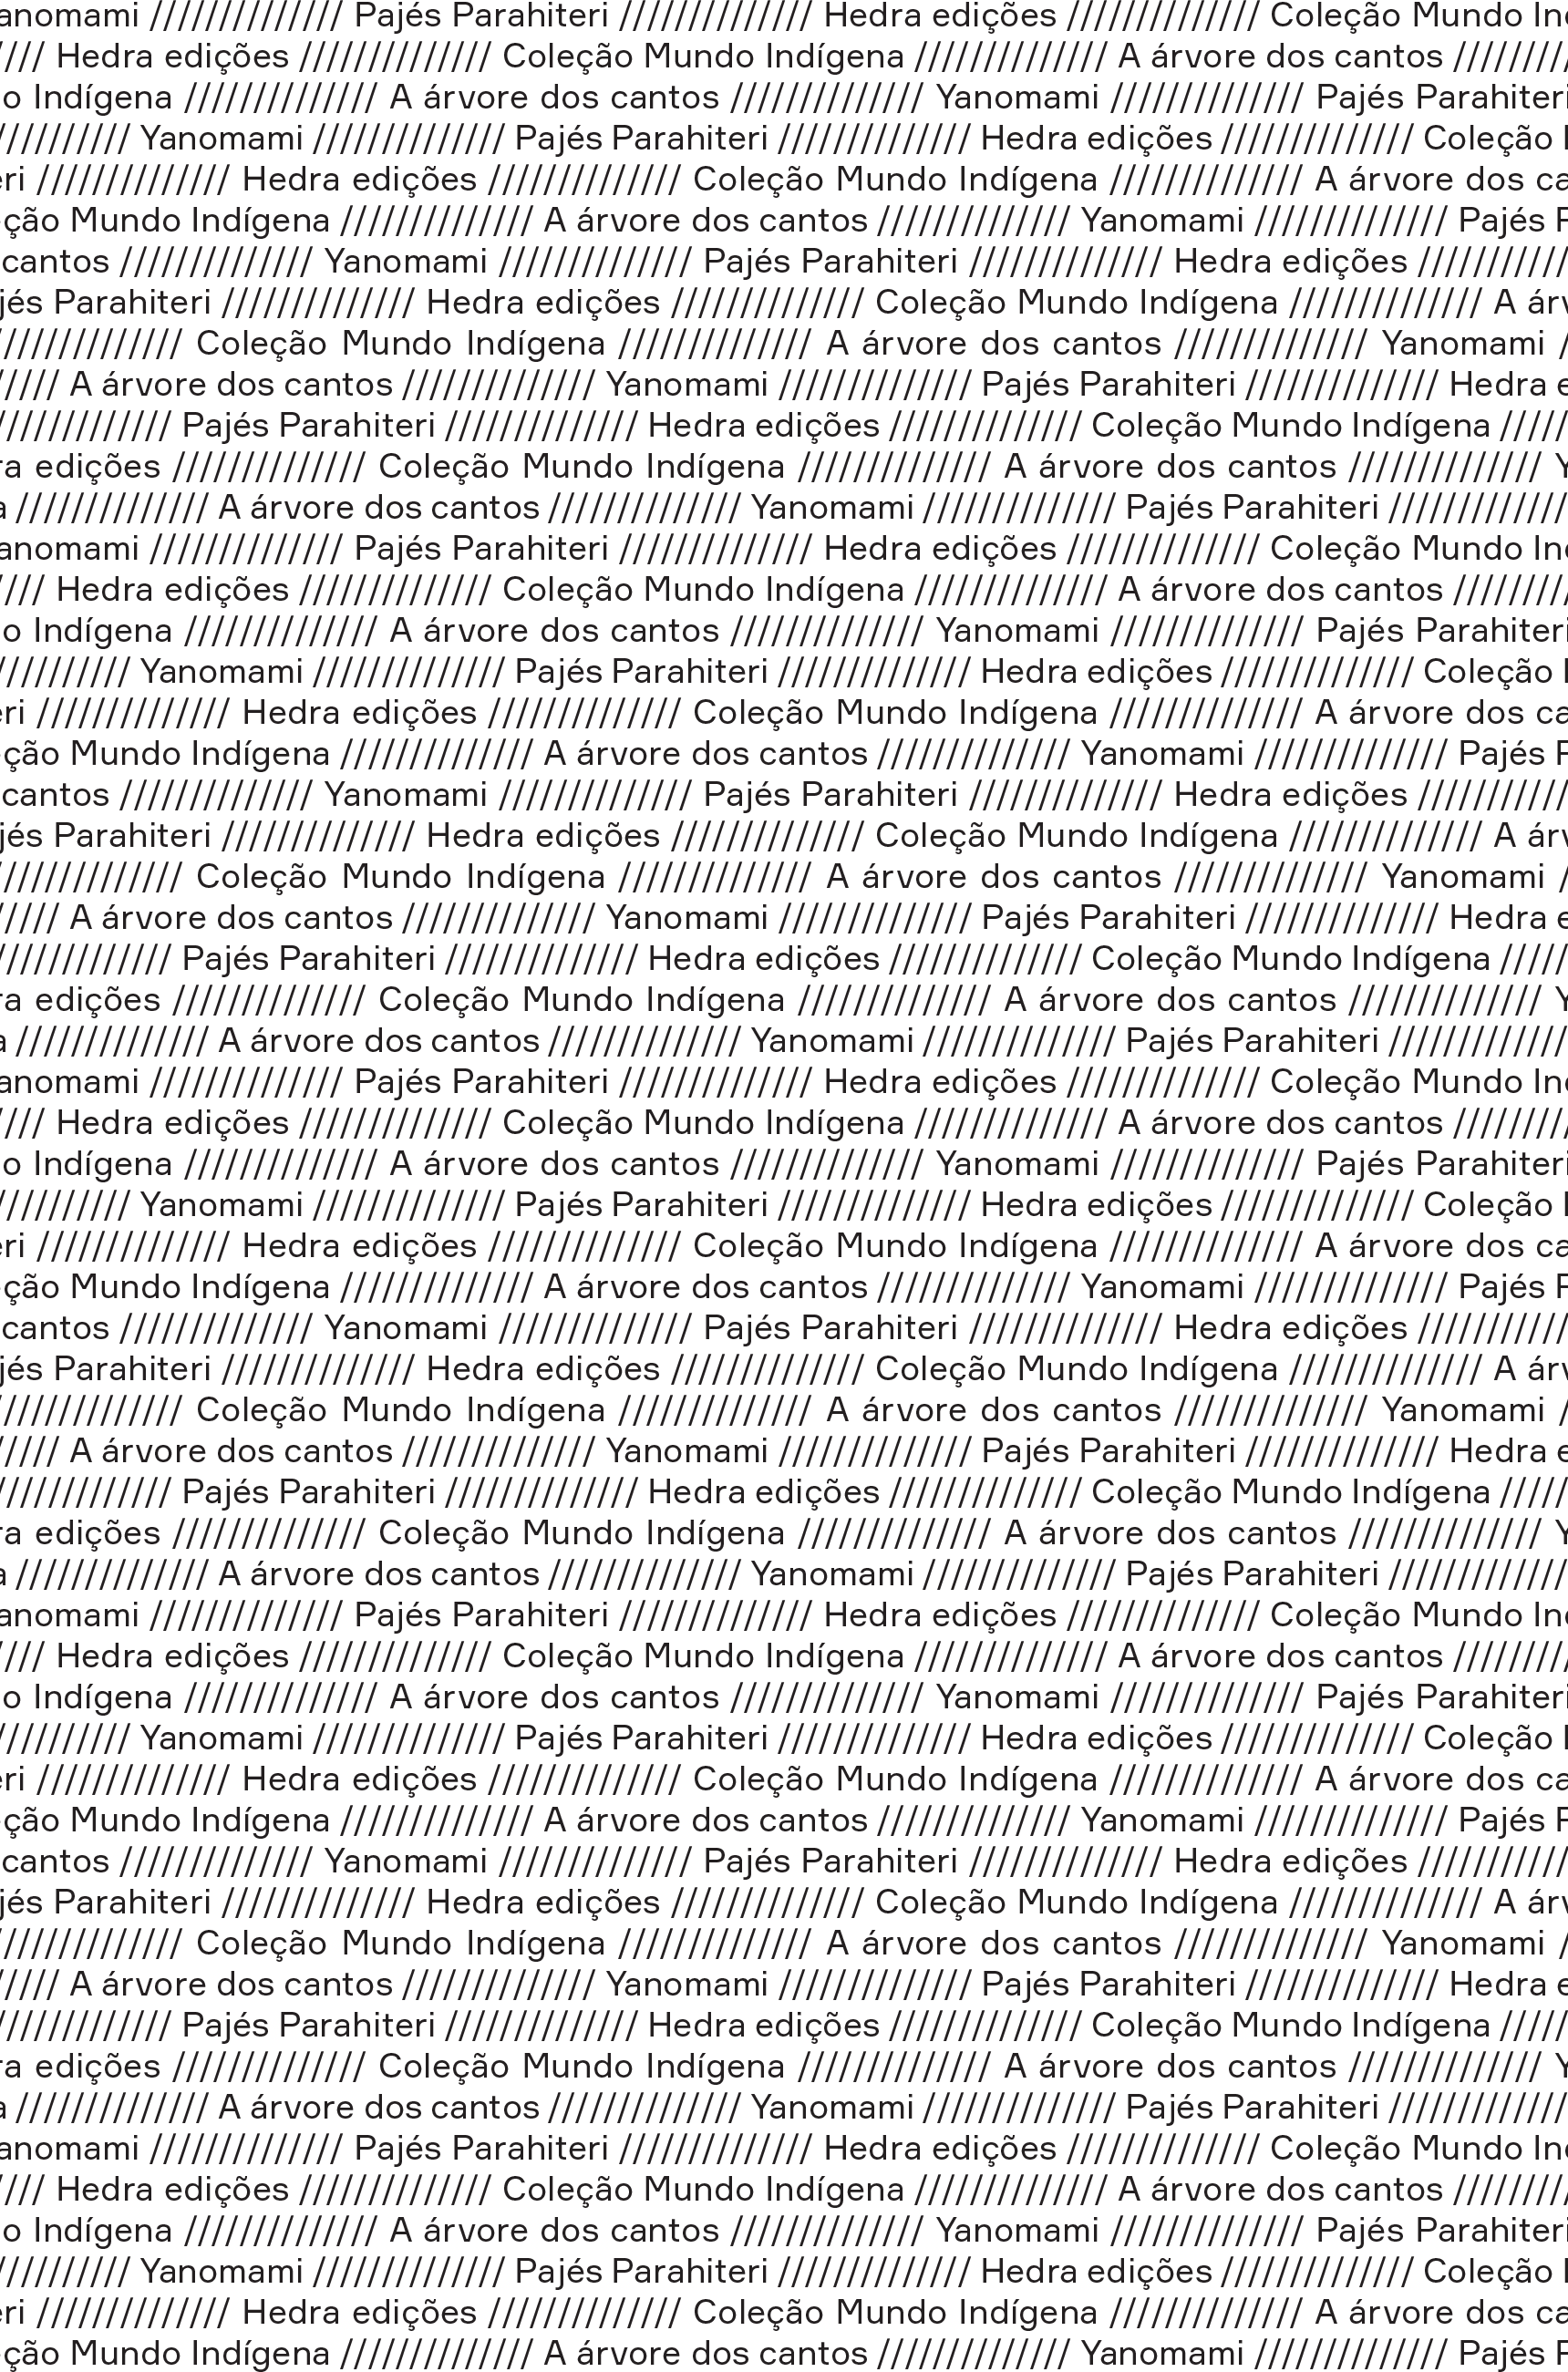
\includegraphics[width=138mm]{./ABERTURA.png}  
\end{textblock*}

\pagebreak
\blankpage

\thispagestyle{empty}
\end{comment}

%\blankpage

% Tamanhos
% \tiny
% \scriptsize
% \footnotesize
% \small 
% \normalsize
% \large 
% \Large 
% \LARGE 
% \huge
% \Huge

% Posicionamento
% \centering 
% \raggedright
% \raggedleft
% \vfill 
% \hfill 
% \vspace{Xcm}   % Colocar * caso esteja no começo de uma página. Ex: \vspace*{...}
% \hspace{Xcm}

% Estilo de página
% \thispagestyle{<<nosso>>}
% \thispagestyle{empty}
% \thispagestyle{plain}  (só número, sem cabeço)
% https://www.overleaf.com/learn/latex/Headers_and_footers

% Compilador que permite usar fonte de sistema: xelatex, lualatex
% Compilador que não permite usar fonte de sistema: latex, pdflatex

% Definindo fontes
% \setmainfont{Times New Roman}  % Todo o texto
% \newfontfamily\avenir{Avenir}  % Contexto
\begingroup\thispagestyle{empty}\vspace*{.05\textheight} 

              \formular
              \Huge
              \noindent
              \textbf{A árvore dos cantos}
              
              \vspace{0.3em}

              \noindent\large\textit{Ou o livro das transformações contadas pelos yanomami do grupo Parahiteri}
                    
\endgroup
\vfill
\pagebreak       % [Frontistício]
\newcommand{\linha}[2]{\ifdef{#2}{\linhalayout{#1}{#2}}{}}

\begingroup\tiny
\parindent=0cm
\thispagestyle{empty}

\textbf{edição brasileira©}\quad			 {Hedra \the\year}\\
\textbf{organização e tradução\,©}\quad	 	 {Anne Ballester Soares}\\

\textbf{coordenação da coleção}\quad		 {Luísa Valentini}\\
\textbf{edição}\quad			 			 {Jorge Sallum}\\
\textbf{coedição}\quad			 			 {Suzana Salama}\\
\textbf{revisão}\quad			 		 	 {Luísa Valentini e Vicente Sampaio}\\
\textbf{capa}\quad			 				 {Lucas Kröeff}\\
%\textbf{assistência editorial}\quad		 {Julia Murachovsky}\\

\textbf{\textsc{isbn}}\quad			 				 {978-65-89705-69-7}\smallskip

\vfill

\begin{minipage}{7cm}
\textbf{Dados Internacionais de Catalogação na Publicação (\textsc{cip})\\
(Câmara Brasileira do Livro, \textsc{sp}, Brasil)}

\textbf{\hrule}\smallskip

Pajés Parahiteri\\

\textit{A árvore dos cantos}. Pajés Parahiteri. Organizado e traduzido por Anne Ballester.\\ 
2.\,ed. São Paulo, \textsc{sp}: Hedra, 2025.\\

\textsc{isbn} 978-65-89705-69-7\\

1.\,Conto. 2.\,Literatura brasileira. \textsc{i}.\,Pajés Parahiteri. \textsc{ii.} Ballester, Anne. \textsc{iii.}\,Título.\\

\hfill \textsc{cdd}: 869.93

\textbf{\hrule}\smallskip

\textbf{Elaborado por Janaina Ramos (\textsc{crb} 8/\,9166)}\\

\textbf{Índices para catálogo sistemático:}\\
\textsc{i.} Conto: Literatura brasileira


\end{minipage}

\vfill

\textit{Grafia atualizada segundo o Acordo Ortográfico da Língua\\
Portuguesa de 1990, em vigor no Brasil desde 2009.}\\

\textit{Direitos reservados em língua\\
portuguesa somente para o Brasil}\\

\textsc{editora hedra ltda.}\\
Av.~São Luís, 187, Piso 3, Loja 8 (Galeria Metrópole)\\
01046--912 São Paulo \textsc{sp} Brasil\\
Telefone/Fax +55 11 3097 8304\\\smallskip
editora@hedra.com.br\\
www.hedra.com.br\\
\bigskip

Foi feito o depósito legal.

\endgroup
\pagebreak     % [Créditos]
% Tamanhos
% \tiny
% \scriptsize
% \footnotesize
% \small 
% \normalsize
% \large 
% \Large 
% \LARGE 
% \huge
% \Huge

% Posicionamento
% \centering 
% \raggedright
% \raggedleft
% \vfill 
% \hfill 
% \vspace{Xcm}   % Colocar * caso esteja no começo de uma página. Ex: \vspace*{...}
% \hspace{Xcm}

% Estilo de página
% \thispagestyle{<<nosso>>}
% \thispagestyle{empty}
% \thispagestyle{plain}  (só número, sem cabeço)
% https://www.overleaf.com/learn/latex/Headers_and_footers

% Compilador que permite usar fonte de sistema: xelatex, lualatex
% Compilador que não permite usar fonte de sistema: latex, pdflatex

% Definindo fontes
% \setmainfont{Times New Roman}  % Todo o texto
% \newfontfamily\avenir{Avenir}  % Contexto

\begingroup\thispagestyle{empty}\vspace*{.05\textheight} 

              \formular
              \Huge
              \noindent
              \textbf{A árvore dos cantos}

              \bigskip  
              
              \large
              \noindent
              \textit{Ou o livro das transformações contadas\\pelos Yanomami do grupo Parahiteri}
              \vspace{11.8em}
              
              \newfontfamily\minion{Minion Pro}
              {\selectfont\minion\small\noindent Anne Ballester (\textit{organização})}

              \bigskip

              \noindent
              {\selectfont\minion\small\noindent 2ª edição}

              \vfill

              \newfontfamily\timesnewroman{Times New Roman}
              {\noindent\fontsize{30}{40}\selectfont \timesnewroman hedra}

              \noindent{\selectfont\minion\small
              \noindent São Paulo \quad\the\year}

\endgroup
\pagebreak
	       % [folha de rosto]
% nothing			is level -3
% \book				is level -2
% \part				is level -1
% \chapter 			is level 0
% \section 			is level 1
% \subsection 		is level 2
% \subsubsection 	is level 3
% \paragraph 		is level 4
% \subparagraph 	is level 5
\setcounter{secnumdepth}{-2}
\setcounter{tocdepth}{0}

% \renewcommand{\contentsname}{Índex} 	% Trocar nome do sumário para 'Índex'
%\ifodd\thepage\relax\else\blankpage\fi 	% Verifica se página é par e coloca página branca
%\tableofcontents*

\pagebreak
\begingroup \footnotesize \parindent0pt \parskip 5pt \thispagestyle{empty} \vspace*{-0.5\textheight}\mbox{} \vfill
\baselineskip=.92\baselineskip
A Coleção Mundo Indígena reúne materiais produzidos com pensadores de
diferentes povos indígenas e pessoas que pesquisam, trabalham
ou lutam pela garantia de seus direitos. Os livros
foram feitos para serem utilizados pelas comunidades envolvidas na sua
produção, e por isso uma parte significativa das obras é bilíngue. 
Isso garante também a divulgação da imensa diversidade linguística dos povos
indígenas no Brasil, que compreende mais de 150 línguas pertencentes a mais de
20 troncos linguísticos.

Caso você tenha gostado do que aprendeu neste livro e queira usar alguma
história ou conhecimento, por favor entre em contato com a editora 
para pensarmos juntos com as comunidades. Lembre-se por favor
que mitologia, neste caso, não é questão autoral tampouco domínio público.\par

\endgroup

\pagebreak\thispagestyle{empty}\movetooddpage
{\begingroup\mbox{}\pagestyle{empty}
\pagestyle{empty} 
% \renewcommand{\contentsname}{Índex} 	% Trocar nome do sumário para 'Índex'
%\ifodd\thepage\relax\else\blankpage\fi 	% Verifica se página é par e coloca página branca
\addtocontents{toc}{\protect\thispagestyle{empty}}
\tableofcontents*\clearpage\endgroup}

\chapter{Apresentação}

\letra{E}{ste} livro reúne histórias contadas por pajés yanomami do rio Demini, sobre os tempos antigos, quando seres que hoje são animais e espíritos eram gente como os Yanomami de hoje. Estas histórias contam como o mundo veio a ser como ele é agora. 

Trata-se de um saber sobre a origem do mundo e dos conhecimentos dos Yanomami que as pessoas aprendem e amadurecem ao longo da vida, por isto este é um livro para adultos. As crianças yanomami também conhecem estas histórias, mas sugerimos que os pais das crianças de outros lugares as leiam antes de compartilhá-las com seus filhos.

\chapter{Como foi feito este livro}

% \begin{flushright}
% \textsc{anne ballester soares}
% \end{flushright}

\noindent{}Os Yanomami habitam uma grande extensão da floresta amazônica, que cobre
parte dos estados de Roraima e do Amazonas, e também uma parte da
Venezuela. Sua população está estimada em 35 mil pessoas, que falam
quatro línguas diferentes, todas pertencentes a um pequeno tronco
linguístico isolado. Essas línguas são chamadas yanomae, ninam, sanuma e
xamatari.

\textls[20]{As comunidades de onde veio este livro são falantes da língua xamatari
ocidental e ficam no município de Barcelos, no estado do Amazonas, na
região conhecida como Médio Rio Negro, em torno do rio Demini. }

\section{da transcrição à tradução}

\textls[-10]{Em 2008, as comunidades Ajuricaba, do rio Demini, Komixipɨwei, do rio
Jutaí, e cachoeira Aracá, do rio Aracá --- todas situadas no município
de Barcelos, estado do Amazonas --- decidiram gravar e transcrever todas
as histórias contadas por seus pajés. Elas conseguiram fazer essas
gravações e transcrições com o apoio do Prêmio Culturas Indígenas de
2008, promovido pelo Ministério da Cultura e pela Associação Guarani
Tenonde Porã.}

\textls[-10]{No mês de junho de 2009, o pajé Moraes, da comunidade de Komixipɨwei,
contou todas as histórias, auxiliado pelos pajés Mauricio, Romário e
Lauro. Os professores yanomami Tancredo e Maciel, da comunidade de
Ajuricaba, ajudaram nas viagens entre Ajuricaba e Barcelos durante a
realização do projeto. Depois, no mês de julho, Tancredo e outro
professor, Simão, me ajudaram a fazer a transcrição das gravações, e
Tancredo e Carlos, professores respectivamente de Ajuricaba e
Komixipɨwei, me ajudaram a fazer uma primeira tradução para a língua
portuguesa.}

\textls[5]{Fomos melhorando essa tradução com a ajuda de muita gente: Otávio
Ironasiteri, que é professor yanomami na comunidade Bicho"-Açu, no rio
Marauiá, o linguista Henri Ramirez, e minha amiga Ieda Akselrude de
Seixas. Esse trabalho deu origem ao livro \textit{Nohi patama Parahiteri
pë rë kuonowei të ã} --- \textit{História mitológica do grupo Parahiteri},
editado em 2010 para circulação nas aldeias yanomami do Amazonas onde se
fala o xamatari, especialmente nos rios Demini, Padauiri e Marauiá. Para quem quer conhecer melhor a língua xamatari, recomendamos os trabalhos de Henri Ramirez e o \textit{Diccionario enciclopedico de la lengua yãnomãmi}, de Jacques Lizot.  }

\section{a publicação}
 
\textls[-10]{Em 2013, fizemos uma reedição dos textos, retraduzindo, anotando e ordenando as narrativas para apresentá-las para adultos e para crianças de todo
o Brasil. Assim, o livro original deu origem a diversos livros com as muitas
histórias contadas pelos pajés yanomami.  Com a ajuda do \textsc{proac},
programa de apoio da \textsc{secult--sp} e da antropóloga Luísa Valentini, que organiza a
coleção Mundo Indígena, publicamos uma versão bilíngue das principais
narrativas coletadas, com o digno propósito de fazer circular um livro que
seja, ao mesmo tempo, de uso dos yanomami e dos \textit{napë} --- como eles nos chamam. }

\textls[20]{Este livro, assim como o volume do qual ele se origina, é dedicado com afeto à memória de nosso amigo, o indigenista e antropólogo Luis Fernando Pereira, que trabalhou muito com as comunidades yanomami do Demini.}
\chapter{Para ler as palavras yanomami}


Foi adotada neste livro a ortografia elaborada pelo linguista Henri Ramirez, que é a mais utilizada no Brasil e, em particular, nos programas de alfabetização de comunidades yanomami. Para ter ideia dos sons, indicamos abaixo.

\bigskip

\begingroup%\footnotesize
\begin{tabular}{rl}
/ɨ/ & vogal alta, emitida do céu da boca, próximo a \textit{i} e \textit{u}\\
/ë/ & vogal entre o \textit{e} e o \textit{o} do português\\
/w/ & \textit{u} curto, como em \textit{língua}\\
/y/ & \textit{i} curto, como em \textit{Mário}\\
/e/ & vogal \textit{e}, como em português\\
/o/ & \textit{o}, como em português\\
/u/ & \textit{u}, como em português\\
/i/ & \textit{i}, como em português\\
/a/ & \textit{a}, como em português\\
/p/ & como \textit{p} ou \textit{b} em português\\
/t/ & como \textit{t} ou \textit{d} em português\\
/k/ & como \textit{c} de \textit{casa}\\
/h/ & como o \textit{rr} em \textit{carro}, aspirado e suave\\
/x/ & como \textit{x} em \textit{xaxim}\\
/s/ & como \textit{s} em \textit{sapo}\\
/m/ & como \textit{m} em \textit{mamãe}\\
/n/ & como \textit{n} em \textit{nada}\\
/r/ & como \textit{r} em \textit{puro}\\
\end{tabular}
\endgroup
\part{A árvore dos cantos}
\part{A árvore dos cantos}

\chapter{A árvore dos cantos}

\letra{N}{ós} \textls[10]{vamos cantar. No início, não havia canto, não havia, ninguém
cantava. Onde se erguia a árvore dos cantos, os dois foram caçar. Dois
moços Wakusitari --- dois não, um só moço, que a descobriu em sua região.}

\textls[10]{Os Katarowëteri eram os amigos dos Yãrusi, cujo líder se chamava Yãrusi.
 Do outro lado da planície, eles, os Wakusitari encontraram a árvore dos
 cantos.} 

\textls[20]{Outros dizem que foram os Koteahiteri que descobriram a árvore cantando,
 e que chamaram os Katarowëteri para pegar os cantos.}

Graças à árvore, os Koteahiteri se enfeitaram com penas de cauda de
papagaio, pintaram-se com elegância, colocando crista de mutum, e
dançaram. Era uma região bonita e plana onde crescia somente a planta
ária. Eles ocupavam uma bela região. 

Por isso, dois moços koteahiteri foram caçar. 

--- Vamos entrar na mata, lá adiante! 

O irmão mais velho e o irmão mais novo foram caçar. A floresta parecia
mais baixa por causa da luz forte, como a luz do dia na roça. Foram
embora naquela direção, andando. Andavam no meio do brejo, andavam no
meio, ouviram os ecos dos cantos. 

\textls[10]{Não havia sujeira no chão onde encontraram a árvore dos cantos dançando,
 para frente e para trás. Havia somente areia bonita e muito brilhante. A
 árvore dançava.} 

\textls[15]{--- \textit{Ãë, ãë, ãë, e, e, e, e, e, ãë, ãë, ãë, ãë}! --- encontraram a árvore
 cantando assim.} 

--- \textit{Ë, aëë, ëaëë, ëaëë, ëaëë, ëaëë, ëaëë}! --- cantava a árvore. 

\textls[-20]{Enquanto isso, o irmão katarowëteri, o filho mais velho, disse:}\looseness=-1 

\textls[7]{--- \textit{Õo}, irmão menor! Dá pra ouvir um canto, lá onde há uma luz grande
 acima do pântano, o som do canto vibra lá, escute isso! Provavelmente é
 o som de um grande monstro! Esse som, naquela direção, mais adiante!
 Vamos nos aproximar por ali, abrir um caminho no areal! Venha aqui!
 Vamos, irmão menor! Vamos logo olhar de perto!} 

--- Será voz de gente? --- disseram os dois. 

Onde a árvore dançava, a luz forte batia na areia bonita. 

\textls[15]{--- \textit{Õoooãaaa}! Vamos, irmão menor, vamos! A árvore dos cantos está
 dançando, vamos, vamos, vamos até nosso pai, para avisá-lo! --- disse.} 

\textls[10]{O irmão menor subiu em uma árvore bonita \textit{matomɨ} inclinada, para
 ver se havia gente por perto, se via algum movimento, subiu e ficou
 no alto.} 

\textls[10]{Ali, na areia, a luz brilhava de todas as cores, repousava bem no
 centro, e a árvore dançava devagar para frente e para trás, cantando. A boca da árvore era bem bonita, e a árvore dançava para frente e para trás.} 

O irmão menor desceu e disse:

\textls[10]{--- \textit{Õooãaaa}! Irmão mais velho! Irmão mais velho! Nossa! Está lá cantando
 e dançando, de uma maneira tão bonita, é a árvore dos cantos! Querido,
 parece que essa árvore canta, essa árvore tem cantos bonitos!} 

--- Vamos! Vamos até nosso pai! 

Os dois disseram e correram imediatamente. Chegaram correndo.

--- \textit{Prohu}! Chegamos! 

Eles encontraram esse som e se enfeitaram por causa da árvore dos cantos. 

\textls[7]{--- Meus queridos! Enfeitem-se para pegarem cantos bonitos! --- disse o
 líder dos Koteahiteri.} 

\textls[10]{O irmão mais velho fez o \textit{himou} com o pai, contando-lhe sobre a
árvore dos cantos.}\footnote{O \textit{himou} é uma modalidade de diálogo cerimonial usada para trazer notícias, ou fazer um convite para uma festa.}

\textls[7]{--- \textit{Tãrai}! \textit{Ha}! Meu pai! Pai! Olhe! Sou teu filho, olhe! Você não sabe
 por que voltei logo correndo! Você nem sabe! Pai! Pai! Pai! Você nem
 imagina o canto bonito que meus ouvidos ouviram! De arregalar os olhos!
 Meu pai! Meu pai! Meu pai! Você que mora aqui, eu sou seu filho, eu não
 lhe diria para proibir as mulheres se enfeitarem! --- disse.} 

\textls[7]{--- É claro! É claro! Queria ouvir isso mesmo, meu filho mais velho,
 querido! --- respondeu seu pai.} 

Fez o \textit{himou}: 

--- Vamos! \textit{Õoooãaaaaõoãaõoãa}! Ele viu uma bonita árvore dos cantos!
\textit{Õõoo}! --- gritaram. 

Ficaram animados.

\chapter{Amoa hi ã he rë haanowehei}

\letra{A}{moa} \textls[15]{pëma a tapë. Hapa amoa a kuonomi. Kuonomi, ai të pë kãi amoamonomi,
tëhë amoa kama hi rë upraatayowei hamɨ, kɨ ramɨ hupɨrayoma. }

Kutaenɨ hi ã eë hapɨrema Wakusitari a huyanɨ, kɨpɨnɨ mai, yami a huyanɨ.
Katarowëteri pë rë kui, Yãrusi kama nohi e pë wãha kuoma, Yarusi përɨamɨ
a wãha kuoma yaro. Ɨhɨ ai maxi yarɨ hamɨ Wakusitari pënɨ amoa hi ã he
haremahe.

\textls[-20]{Ɨnaha ai të pë kuɨ: Hei Koteahiteri pë yainɨ amoa kë hĩ ã he haamahe.
 Katarowëteri kë pë ha nakarëhenɨ, amoa kë hĩ ã toamahe.}\looseness=-1 

Amoa hi nohi pauxiamahe. Werehi xina pata huuhamahe. Pë onimoma, pë no
aiama, ɨ̃kɨmo a huuhamahe, pë ha kuaanɨ, amoa hi nohi praɨamahe. Urihi
katehe kë, kuma kë masi he pata yarɨmoma, urihi katehe a pomahe. 

\textls[15]{Pouhe yaro, ɨ̃hɨ Koteahiteri huyahuya kɨ ramɨ apɨyo hërɨma. Kɨ ramɨ ha
 apɨro hërɨnɨ.} 

--- Kiha pëhë kɨ ha paikutunɨ! 

Hei pë pata, hei pë oxe, ɨnaha ramɨ kë kɨ hupɨma, ramɨ kë kɨ apɨyo
hërɨma. Kutaenɨ, hɨ̃ɨɨ! e të xĩi pata yahatotoa hërɨma. Hikari kurenaha e
të xĩi pata kuaa hërɨma. Kuaa hërɨpë hamɨ, kɨpɨ katito hërɨma. Matotapɨ
hërɨma. 

\textls[10]{Yãmaro kë xĩi pata hamɨ kɨ mɨ amopɨa hërɨma, mɨ amopɨa hërɨɨweiiiiiii,
 mɨ amo yai ha amoa kë ã wa karëhoma, mɨ amo yai ha hẽka a praopë ha
 kunomai, amoa kë hi tirurou he hapɨrema, makamaka katehe kë a pata
 yaixĩi no aihimou totihiopë hamɨ, amoa kë hi tiruroma.} 

\textls[-7]{--- \textit{Ãë, ãë, ãë, e, e, e, e, e, ãë, ãë, ãë, ãë!} --- amoa e hi kupɨɨ he
 harema. --- \textit{Ë, aëë, ëaëë, ëaëë, ëaëë, ëaëë, ëaëë!} --- amoa e hi kupɨma.
 Kuɨ ha, Katarowëteri pata a rë kui, ihirupɨ pata e rë kui:}\looseness=-1

\textls[7]{--- \textit{Õo!} Õasi! Amoa a nohi karëhorati kihi të xĩi pata rë makerati ha,
 kihi amoa, kiha amoa kë a morokaɨ kurati, yɨmɨka ta taprao, ɨ̃hɨ rë --- e
 kuma --- Yai të ã pata pë wëë! --- pata e kuapraroma. Ɨhɨ Koteahiteri
 pënɨ. --- Kihi të ã rë morokarati hamɨ, mihi të pata makamakapɨ rë
 matoto piyëhërɨ hamɨ, wa yo ha reikimapaharunɨ, a ta ahehetetaru! ---
 pata e rë kuyaronowei --- Pei! Oxei! Pëhë të ta mɨɨ ahetou xoao!} 

--- Yanomamɨ rë të pë ã mata tawë! 

Kɨ noã tapɨyoma, amoa kë hi tirurupë hamɨ. \textit{Hɨ̃ɨɨɨɨɨ! }Makamaka katehe kë e
xĩi pata makeoma. 

\textls[-20]{--- \textit{Õooãaaa}, pei kë, oxei, pei kë oxei, amoa hi rë tiruropiyei ë, pei
 kë, pei kë, hayë kë ihamɨ ëë, hayë pëhë a yɨmɨkamapëë! --- e kuma.}\looseness=-1 

\textls[-20]{Matomɨ katehe hi pata kaɨopë hamɨ, oxe e tukema, Yanomamɨ të pë mɨɨ ha,
 të pë xurirou mɨɨ ha, e ha tuikunɨ, e ha tirehetarunɨ.}\looseness=-1 

Kihi makamaka kë a xĩi pata no aiwë makeaɨ kupiyei, mɨ amo yai hamɨ amoa
kë hi wa kãi opi tirutirumoma, të hi kahikɨ no aiwë no kirii, e të hi
tiruroma. 

\textls[-20]{--- \textit{Õooãaa!} --- e ha nihoroto hërɨnɨ --- Apa! Apa! Kurahë katehe kë të
 wã kãi tirurou kuopiyei. Apa, amoa kë hi ë! --- a kuma. --- Pusi amoa kë
 hĩ ã no taië, pusi amoa katehe kë hĩ ã rë taië! --- e kuma.}\looseness=-1 

--- Pei kë! Hayë kë ihamɨ ë! Kɨ ha kupɨnɨ, kɨ rërëpɨa xoape hërɨma. Kɨ
ha rërëpɨpo hërɨnɨ: 

--- \textit{Prohu!} --- e kɨ kupɨma. 

Amoa hi nohi pauxiaɨhe ha: 

--- Pusi pei kë pë ta pauximo xë! Amoa katehe wama a toapë! --- përɨamɨ
Koteahiteri e kumahe. 

Hi nohi himopɨama pë patanɨ e hi nohi himoama, amoa hi wãha nohi wëaɨ
ha, pë hɨɨ iha. 

--- \textit{Tãrai!} --- e kuma --- \textit{Ha!} Napemi! Napemi! Ha! Hei yarohë ya rë kuii,
ha! Weti wa të taɨ ha, wa të rërëɨ mɨ yapa a ta kuponɨ? Wa puhi kuoranɨ
ha kunomai! Napemi! Napemi! Napemi! Hei ya yɨmɨka ha amoa katehe ya rë
hiritaɨwei! Ya mamo rë ikeketouwei, napemi! Napemi! Napemi! Hei kɨ suwë
rë kui, kɨ pauximomaɨ mai! E roa yai a ta përa! Yarohë ya rĩya kuoranɨ
kunomai! --- e kuoma. E kuɨ ha: 

--- Hão! Hãooooo! Noa taɨ yai a ta përaxëa. Pusiwë! Pusiwë! Ha! Ɨnaha rë
kë, ɨnaha rë kë --- pë hɨɨ e kuma. 

E nohi himoama. 

--- Pei kë! \textit{Õoãaõoãaõoãa!} Amoa katehe hi he hõra rë harenowë! \textit{Õoooo!} ---
e pë kuma. 

E pë xi wã kãi toaama.

\chapter{Monstro Këyakëya}
 
\letra{H}{avia} também os que viviam na região centro-sul, os
Yãimoropɨwei, que ficaram presos, pois moravam dentro da terra com o
monstro Këyakëya --- que, portanto, não era gente. 

\textls[10]{Os que asfixiaram Këyakëya existiam bem antes de nossos antepassados.
Këyakëya morava dentro da terra, na vizinhança do \textit{xapono} dos
ancestrais.}\footnote{Os \textit{xapono} são as casas coletivas circulares onde moram os Yanomami. Cada casa corresponde a uma comunidade; em geral não se fazem duas casas numa mesma localidade.} 

Apesar de ser um monstro, Këyakëya era líder dos Yãimoropɨwei. Os
companheiros de Këyakëya moravam dentro da terra e a casa deles tinha um
respiradouro, como o da casa do tatu. A casa de Këyakëya também tinha um
respiradouro. Moravam ali também os Motuxi, que se dividiram e se
espalharam. 

\textls[15]{Os Prãkiawëteri asfixiaram Këyakëya, tentando matá-lo. Asfixiaram-no,
 foi assim que nos ensinaram a matar. Eles não o mataram com flecha.} 

No início, não havia matança, não havia inimizade, não havia briga
mortal. Os \textit{napë} também não existiam.\footnote{O termo \textit{napë} designa os estrangeiros, em geral os brancos, ou quem adotou seus costumes.} Os nossos antepassados não sabiam manifestar ira nem raiva. 

\textls[-12]{Ele conseguiu escapar sob a forma de espírito. Ele não se transformou à
 toa. Os companheiros dele, como nós, sempre padeciam de fome; todos
 morreram pela fumaça que entrou no buraco.}\looseness=-1

Këyakëya nos legou o sentido de vingança por causa da filha de quem?
Qual é o nome do pai cuja filha foi vítima da crueldade de Këyakëya, que
chegou e entrou no \textit{xapono}? A vítima que, brutalmente, Këyakëya fez
descer da rede e sair era a filha do líder dos Naɨyawëteri. Era uma moça
bonita, realmente muito bonita. Ela estava na primeira menstruação e,
mesmo assim, ele a arrancou da reclusão.

\textls[-15]{Apesar de ser monstro, Këyakëya existia e vivia como gente. Como
 morava dentro de um buraco, depois de trucidar a menina menstruada, ele
 e os demais membros do grupo foram asfixiados pelos Prãkiawëteri. Mas
 apenas Këyakëya conseguiu fugir, se tornando eterno na forma de
 espírito. Ele ainda existe como espírito.}\looseness=-1

Naɨyawë desgalhava um pé de fruta \textit{naɨ}\footnote{ Segundo Lizot, uma balateira, \textit{Manilkara bidentata}.} em uma roça
distante. \textit{Aooo, aoooo, aoooo, aooo}! Fazia assim para sua gente. 

\textls[-20]{Enquanto eles comiam a fruta \textit{naɨ}, Këyakëya arrancou a menina do
 seu recluso, matou-a e a devorou. Ele a comeu sozinho.}\looseness=-1

\textls[-20]{Fez lascas pequenas da carne das demais crianças, que também havia
 trucidado, para oferecer a todos seus companheiros. Amontoou as lascas de
 carne que ele colocou no seu grande cesto, chamado \textit{yotema}.
 Carregou todos os restos das crianças massacradas e levou junto o irmão
 da menina menstruada, que estava vivo e bonito. Ele o fez sentar em cima
 dos cadáveres dentro do cesto.}\looseness=-1 

\textls[-20]{O menino vivo, que ele levou, transformou-se em papagaio durante o
 percurso. Këyakëya saiu do \textit{xapono} dos Naɨyawëteri e andava a passos
 largos, foi então que o menino, já de longe, disse:}\looseness=-1

--- \textit{Kuao}! \textit{Kuao}! \textit{Kuao}!

Esse som se tornou o som dos papagaios. Esses pássaros voam; ele pousou
em um galho e assim ficou. Këyakëya olhou para a beira do cesto,
querendo ver se o menino ainda estava sentado. Fez o filho de Naɨyawëse
tornar papagaio. Como o menino não estava, ele retornou àquela direção.
O menino se tornou a imagem do papagaio que grita: \textit{Kuao}! \textit{Kuao}!
\textit{Kuao}!

--- Ouça! Meu xerimbabo! Onde você pousou? \textit{Kuato, kuato, kuato}! ---
disse Këyakëya voltando e correndo. --- Em qual paragem você
ficou? \textit{Kuato, kuato, kuato}!

--- \textit{Õiyaoooo}! --- disse o papagaio. 

\textls[15]{Assim disse aquele que, apesar de ser filho de gente, tornou-se
 papagaio.} 

\textls[-20]{É a história dos antepassados. Também existiam monstros com outros
 \textit{xapono}, sendo essa a história de Këyakëya e dos Yãimoropɨwei, que
 moravam em \textit{xapono} pouco distantes um do outro.}\looseness=-1 

Depois, aparecerá o nome do rio que tirará e levará muitos ancestrais
Yanomami. É somente depois da história dos Yanomami levados pelo rio que
vem nossa história. Os Waika a contam de uma maneira diferente, eles a
contam conforme seus antepassados lhes contaram.\footnote{O par \textit{waika}/\,\textit{xamatari} parece ter sido usado originalmente para designar outros grupos yanomami vivendo em região geográfica diversa de quem fala, os primeiros ao Norte e Oeste, e os segundos ao Sul, reconhecendo-se neles conjuntos de características que os particularizam. Os termos foram atribuídos em diferentes momentos pelos brancos para designar grupos específicos de forma estável e, no caso de \textit{xamatari}, para designar a própria língua do tronco yanomami usada pelos Parahiteri que fizeram este livro.} 

\textls[10]{Os companheiros de Këyakëya não sobreviveram, morreram todos pela
 fumaça. Eles os asfixiaram a todos, somente Këyakëya sobreviveu, se
 transformando em espírito eterno. Esse sobrevivente alcançou o \textit{xapono} dos
 espíritos, pois se tornou um deles, quando ainda eram Yanomami e moravam
 como nós. Ele os alcançou e ficou lá.} 

Não mora mais onde o asfixiaram. Somente restou o marco dele. Não pensem
que os companheiros de Këyakëya sobreviveram e se agruparam enquanto ele
alcançava os espíritos! 

Não houve sobreviventes do grupo dos Naɨyawëteri. Acontecerá depois. Os
sobreviventes eram os que afundaram, não os outros antepassados. As
águas sobem devagar e os que afundam são os únicos sobreviventes. 

\enlargethispage{1\baselineskip}

Depois, os que tinham o mesmo nome que as montanhas também
sobreviveram.

\chapter{Këyakëya}

\letra{K}{ama} pë rë kuonowei koro ha mɨ amo ha, pë xi rë wãrionowei, pë rii rë
titionowei, yai tënɨ pë kãi titioma. Këyakëya, Yanomamɨmi makui, a
përɨoma. 

\textls[10]{A rë yarënowehei. Kamiyë pëma kɨ no patapɨ përɨo mao tëhë, të pë rë
 përɨo xomaonowei të pë wãha xomaa. Ɨhɨ pata pë yahipɨ he tikë ha,
 pëɨxokɨ ha, yai të titioma.} 

Këyakëya përɨamɨ a wãha, yai të makui. Ɨhɨnɨ Yãimoropɨweiteri pë kãi
përɨoma. Këyakëyanɨ pë kãi rë titionowei, mahu hẽremopɨ kuoma, opo pë
hẽremopɨ rë kurenaha Këyakëya yai të hẽremopɨ kuoma kutaenɨ, Motuxi pë
pata xereremou piyëkëmoma kutaenɨ, kama e pë kãi rë përɨonowei,
Motuxiwëteri pë kãi titioma. Këyakëya ei pë wãha. 

Wetinɨ Këyakëya pë kãi rë titiaɨwei, weti naha pë wãha kuoma? Ɨhɨ
Prãkiawëteri pënɨ Këyakëya a yarëmahe, a xëpraremahe. Ɨhɨ pënɨ pëma kɨ
ixou hiraɨhe ha, Yãimoropɨweiteri pënɨ Këyakëya a unokai yarëmahe. A xëprapehe, a yarëmahe, kamiyë pëma kɨ xëprayopë. A nianomihe. 

Hapa niayou të kuonomi. Pëma kɨ napëmayou, xëpraɨ të kuonomi. Napë pë
makui, pë kãi kuonomi. Pëma kɨ nohi patama waiterimou taonomi, huxuo kãi
taonomi, ɨ̃hɨ pë xëremahe. 

\textls[-20]{Këyakëya a xëpraɨ puhioma makuhei, a xëpranomihe. A hekura tokua he
 yatirayoma, kama a kuprou pëonomi. Hei kamiyë kureneha kuwë të pë no
 xĩro preaama, të pë hɨtɨtɨwë nomarayoma.}\looseness=-1 

Këyakëyanɨ weti tëëpɨ noã prearema? Këyakëyanɨ pë tëë e napë rë
itorayonowei, e napë rë harayonowei, weti naha pë hɨ̃ɨ e wãha kuoma?
Naɨyawëteri ihirupɨ, tëëpɨ noã prearema. Kama përɨamɨ Naɨyawëteri a yai
kuoma. Suwë katehe a yai kuoma. Pë tëë e yai riëhëoma, kamiyë kurenaha
mai! Ɨhɨ suwë katehe yɨpɨ a ha ukëa he ha yatirënɨ, a noã prearema. 

Ɨhɨ a përɨoma, Këyakëya a rë përɨonowei, yai të makui Këyakëya a
Yanomamɨ përɨoma. A titioma kutaenɨ, ɨnaha të tama yaro, yɨpɨ hena
xëpraɨ xi ha wãrironɨ, kama e pë rë kui, e pë no ha prerarunɨ, e pë ha
yarërarɨhenɨ, kama a rë kui a parimi hekura tokua xoarayoma. Ɨhɨ a hëa
xoaa, hekura. 

\textls[-20]{Kihi hikari a rë kurahari naha, naɨ a pehi pata tihetimamahe ha:}\looseness=-1

--- \textit{Ãooo, ãoooo, ãoooo, ãooo!} --- Naɨyawëteri e pë kuma. 

Naɨ a waɨhe tëhë, a ukëa hearema. A xëprapë, a wapë. A warema. Yaminɨ a
warema. 

\textls[-10]{Nakaxi yãhi pë wai ha tanɨ, tanɨ, kama urihiteri pë haikama, pë
 topërarema. E yãhi kɨ ha orɨhenɨ. Pë ihirupɨ pë no mapraɨ hearayoma
 yaro, hɨtɨtɨwë pë mɨ këa heararema, pë yehire hërɨma, kama yotema e
 hamɨ. Ihiru e pë no payeri rë tapraɨwei, pë titire hërɨma. Ɨhɨ pë taɨ
 makure, a rë përɨaɨwei, yaɨpɨ rë këprarɨhe, ihirupɨ e rë kui a yure
 hërɨma. Temɨ. A rë riëhei. E tikëmare hërɨma.}\looseness=-1 

Ei a rë yurehe, kiha a kãi kutou tëhë, werehi e kuprarioma. Hëyëha a kãi
rë hare, a kãi rë rahurahumoimati, kihi karexi si rë prarahari naha a
kãi kutou tëhë: 

--- \textit{Kuao, kuao, kuao!} --- të pë werehi rë kuuwei a no uhutipɨ
kuprarioma, të pë yëɨ ha piyei kunɨ heinaha e ha waroroikunɨ, e kasikɨ
mɨprarema, Këyakëyanɨ, e tikëa mɨɨ ha. Përɨamɨ e ihirupɨ
werehipramarema. A maa ha, e wã kãi yëa mɨ yapakema: 

--- Tãrio, weti ha wa hore piyëkei kuhe? a wãti. Kuato, kuato, kuato!
--- e kuɨ mɨ rërëa mɨ yapakema --- Weti ha a hëprario kuhe? Kuato,
kuato, kuato! 

--- \textit{Õiyaoooo!} --- e kurayoma. Yanomamɨ ihirupɨ kuoma makui, e kua
topramarema, ɨnaha e kuma. 

\textls[-15]{Ɨnaha të ã kua, pata të rë kui, ɨnaha të pë kuaama. Ɨhɨ yai tënɨ pë kãi
 përɨoma, ɨ̃hɨ tëhë ai të pë rë përɨonowei, ɨ̃hɨ të ha, hei Këyakëya a rë
 yarënowehei, Yãimoropɨweiteri pë hirao he paoma.}\looseness=-1

\textls[7]{Ɨhɨ ei rë pë rë kui, waiha pei rë u kë wãha rë taore hamɨ, pë rë
 pakakumare të wãha kupropë. Ɨhɨ rë të he tikë hamɨ, të he tikëatayoa, të
 he tikëa kurati, komosi të ã yai. Hei Waika pë rë kui, maa, kama e të
 rii taɨhe. Kama pë no patapɨ wãha rii tao. Kamiyë pëma kɨ no patapɨnɨ të
 ã rë wëyënowehei ei të ã rii. Të rii ma rë yaitapraruhe. Ɨhɨ kama, ɨ̃hɨ
 të rii maxi hamɨ, ɨ̃naha të kuoma, hapa të pë rë përɨonowei.} 

\textls[7]{Ɨhɨ Këyakëya urihi teri pë rë kuonowei të maxi hamɨ pë rë kuonowei,
 Këyakëya urihiteri pë rë kui, ai e pë hëpronomi, kaɨ wakë xinɨ, pë
 xëpraremahe. Pë yarëpraɨ haikirayomahe yaro, ai pë temɨ haimi, hei pë rë
 kui, Këyakëya kama a rë kui, a hekura ha parimiprarunɨ, a hëtarioma. A nomanomi. Ei a rë kui, hekura pë iha a waroopë, a hëprario kuhe,
 Këyakëya hekura. Yanomamɨ pë kuo tëhë, hei pëma kɨ rë kurenaha hekura pë
 përɨoma. E warokemahe. Ɨha a kuopë.} 

Kama a rë yarënowehei ha a titia xoaami. Hekura yai të pë iha a
warokema. Pei uno kua hëa. Hei pë rë kui, hei pë rë hëpraruhe, hei pë rë
kui, Këyakëya hëyëmɨ e kua rë xoarahai weti naha kuwë të pë hiraopë ha,
Këyakëya a warokema, pë puhi kuu mai! A warokema. 

\textls[-15]{Naɨyawëteri pë rë hëre, hei pë hëtopë mai! Hei pë mixi rë tuore, pë xĩro
 hëprario, ai të pë no patama hëpronomi. Wãisipɨ, ĩsitoripɨ të u wai rë
 õkimouwei, pë mixi rë tuowei pë rë kure, hei kë pë.}\looseness=-1 

Ɨhɨ pë rë kui, te he tikë hamɨ ai pë rii, pei ma pë rë kui, ma pë wãha
rë yehiponowehei, ɨ̃hɨ pë kãi hëprarioma.

\chapter{O surgimento das cobras}
 
\letra{N}{essa} \textls[-7]{época também, as cobras não rastejavam como rastejam hoje, elas
viviam como os Yanomami. Transformaram-se onde desceu o Sangue da Lua,
na floresta. Lá, caíram as cobras que picam. Transformaram-se em cobras
lá em cima, enquanto iam para uma festa. Hoje, quando vocês olham para o
céu, vocês veem o peito daqueles que se transformaram em cobras. Não
havia cobras, nem jiboias, nem sucurijus. Os poraquês não existiam, nem
os peixes. Nós comemos a carne de gente.}\looseness=-1

Eles se transformaram em cobra, não no \textit{xapono}, mas nesta floresta mesmo.
Foram chamados e foram lá, Wataperariwë e Jiboia, o irmão mais velho.
Foram lá longe com as Cobras, mas se transformaram na floresta. Eles,
então, não foram dançar. 

\textls[10]{Com a cabeça coberta de penas brancas, dessa mesma forma que nós nos
 pintamos, cada um pintou seu corpo com listras diferentes. As Cobras
 moravam na sua própria região, como gente. Transformaram-se quando
 foram convidadas a dançar. Elas antes viviam como gente.} 

\textls[-5]{Quem eram os dois \textit{tuxauas}? O irmão mais velho e o irmão mais novo
 moravam com as Cobras. Os dois também foram dançar. Watawatariwë e
 Jiboia moravam com seu grupo, as Cobras. Jiboia era o irmão do meio.
 Watawatariwë era o caçula. Os dois irmãos mais velhos eram esses: Jiboia
 e Sucuriju, que nasceu primeiro. Aqueles que se pintaram eram três, pois
 havia também Watawatariwë, o caçula, por isso nós nos pintaremos assim.}\looseness=-1

Os Parawari também viviam com eles. Por causa deles se metamorfosearam,
porque os Parawari os levaram. 

Todos eles moravam em frente à serra Wãyapoto, que ainda tem esse nome.
Ocupavam essa região ao pé da serra na planície. Eram todos bonitos. É o
nome da região onde moravam os antepassados. É o verdadeiro nome dessa
região. As Cobras bebiam a água do rio Wãyapo, tomavam banho, se lavavam
nesse rio bonito. Tomavam banho e bebiam água. 

\textls[-18]{Eles nos ensinaram, assim, a dançar, mas, infelizmente, se
 metamorfosearam. Eles iriam dançar, mas, infelizmente, se transformaram.
 Iriam dançar. Transformaram-se em cobras imediatamente. Tornaram-se
 cobras. Não foram dançar no \textit{xapono} de outros.}\looseness=-1 

Em que \textit{xapono} iam dançar? No \textit{xapono} daqueles que se transformaram, que ainda existe na terra plana. Aqueles que se transformaram, apesar de se
pintarem fora do \textit{xapono}, sofreram a metamorfose, transformaram-se em
cobras. 

Os que convidaram as Cobras, como se chamavam esses antepassados? Eles
gritavam enquanto cozinhavam o mingau de banana para os visitantes. 

--- Por que estão agindo assim? --- perguntaram-se.

Pareciam gritar de propósito. Transformaram-se perto do \textit{xapono} dos
Jalouaca. Transformaram-se perto desse \textit{xapono}. Transformaram-se. Os
antepassados se chamavam assim, Jalouaca. Assim se chamava o líder. Eram
espíritos, são nomes de espírito. Eram Yanomami e moravam como os
Yanomami. 

Apesar de morarem, 
%onde?
assim como nós, após a metamorfose em cobra eles não
voltaram à condição de seres comuns. Pintaram-se fora do \textit{xapono} dos
Jalouaca, pensando: 

--- Os Yanomami se pintarão assim! 

E se pintaram com listras. Pintaram-se, na parte superior do braço, com
cor de sangue preto, igual à cor de meu irmão mais novo, como a cor de
seu braço. As cobras \textit{maraxari} se pintaram assim; a cobra-coral
também se pintou com manchas vermelhas. 

\textls[-23]{O segundo grupo do \textit{xapono} das Cobras se pintou em outro lugar, distante,
 para que aquelas do outro grupo, que se achavam bonitas, se zangassem.
 Elas tomaram banho no rio Wataperari, cuja água era branca. Ficaram onde
 brilhava a luz. Assim era a luz do rio. Perto do \textit{xapono} dos Jalouaca,
 havia o rio, o rio apareceu de repente.}\looseness=-1

\textls[-30]{Um pouco longe do \textit{xapono}, as outras Cobras se pintavam juntas.}\looseness=-1

\textls[-10]{Pintaram-se. No segundo grupo havia uma mulher. Os bonitos desse
grupo, eram muito bonitos, chegaram até as outras cobras. Chegaram
também com eles dois Parawari bonitos, todos eram muito bonitos.
Chegaram. A beleza de suas pinturas incomodou os outros, que ficaram com
inveja. Chegaram, enquanto os outros se pintavam com riscas. Aquele,
cujo nome eu dei, apareceu no meio deles, Sucuriju. Ele, o irmão mais
velho, estava ao final dos que chegavam, aquele que tem grandes
desenhos.}\looseness=-1

--- \textit{Hɨ̃hɨ̃}! \textit{Wĩsa}! \textit{Wĩsa}! --- assobiaram. 

\textls[-20]{Os do primeiro grupo, ainda se pintando, viraram a cabeça para olhar em
direção das cobras bonitas chegando, e disseram, felizes:}\looseness=-1

--- Acabei de me pintar desse jeito! 

Apesar de não terem dentes como os dos Yanomami, depois de se
transformarem em cobras, depois da metamorfose, os dentes saíram. No
início, não havia cobra, aquelas que picam não andavam no chão, não
havia cobra-surra, nem coral, nem cobra \textit{maraxa}, nem
cobra \textit{huwëmoxi}. Não havia nenhuma dessas cobras. Lá, onde os
bonitos estavam se transformando em cobras, houve um barulho tão grande
como o de um bando de queixadas, pois as cobras estavam surgindo. As
jararacas, as surucucus, as cobras-papagaios e as
cobras \textit{waro} também surgiram. Invadiram toda a floresta. Assim foi. 

Aqueles que haviam convidado as Cobras, os Jalouaca, por causa dos quais
aconteceu a transformação, subiram também ao céu no lugar da
transformação. Os bonitos estavam suspensos. \textit{Torurururu}! E
trovejou. --- \textit{Prohu}! --- Chegaram lá. Não estão aqui, nessa terra,
pois andam lá. Queriam viver saudáveis, então estão lá, saudáveis. Não
ficam em baixo. Ficaram em cima. 

Quando as Cobras subiram, o que aconteceu com os amigos delas, os
Jalouacas? Transformaram-se também em cobra. 

Então, os líderes do primeiro grupo, que se transformaram também
em cobras, ficaram na terra.

\chapter{Të pë rë oruprarionowei}
 
\letra{O}{ru} pë kãi hunomi, oru Yanomamɨ kurenaha pë kãi përɨoma, pë kãi kuoma.
Ɨhɨ, kihamɨ, Pẽripo ĩyë rë itorati hamɨ, urihi hamɨ, kiha pë xi
wãrihotayoma. Ɨha pë oru rë kerayonowei, të pë si wëyëɨhe, oru pënɨ.
Heaka hamɨ, pë xi rii wãrihipraritayoma. Pë praɨaɨ mɨ ha hurɨnɨ, pë xi
rë wãrihonowei, hei wama parɨkɨ mɨɨ. Oru pë hunomi, hetu pë hunomi,
wãikoya pë kãi kuonomi, yahetipa pë kãi kuonomi, yuri pë kãi kuonomi,
Yanomamɨ wama të pë yãhi kɨ waɨ. 

Urihi ha pë ha nakarehenɨ, pë huɨ ha kuikutunɨ, Wataperariwë, Heturiwë
pata xo Oruri pë kãi hupɨɨ ha kuikutunɨ, urihi ha pë xi wãrihoma, pë
praɨɨ kateheonomi. 

\textls[-10]{Pei të pë horoimo pë ha, të pë ma rë yãmouwei, pei të pë pata yãprutaaɨ
 yaitaama, Oruri pë ha oraora ya të wãha takema, korokoro pë wãha kuami,
 pë xi rë wãrihonowei. Ɨhɨ Oruri pë rë kui, kama pë urihipɨ ha, Yanomamɨ
 kurenaha kamiyë pëma kɨ rë kurenaha pë përɨoma, pë xi wãrihiprarioma. Pë
 xi wãrihopë makui, pë praɨɨ mɨ ayoma, pë ha xorehenɨ, Yanomamɨ pë përɨo
 parɨoma.}\looseness=-1 

\textls[10]{Ɨhɨ exi e të përɨamɨ kupɨoma? Pata, pë oxe. Oruri pë kãi rë
 përɨpɨonowei. Ɨhɨ pë kãi praɨpɨɨ mɨ kãi rë hurayonowei, Watawatariwënɨ
 pë kãi përɨoma, Oruri, Heturiwë xo. Heturiwë pata e wãha yai, pëɨxokɨ
 hamɨ ke e. Pata ɨnaha e kɨ kupɨa hei, pë xĩro. Wãikoyariwë pei a haa
 xomarayoma. Ɨnaha pë kua. Ai, ai, ai pë kuoma. Wãikoyariwë e kãi kua,
 kama pë rë onimonowei, kamiyë pëma kɨ onimopë. Wãikoyariwë, Hetu,
 Watawatariwë oxe e wãha, suhe u haikatimɨ.} 

Parawari pënɨ pë kãi hiraomahe, Parawari pë xo pë hiraoma, ɨ̃hɨ pënɨ pë
rurure hërɨmahe yaro, Oruri pë xi wãrihamapehe, katehe kama pë xĩro
hirao yarɨtaoma. 

Wãyapoto a parɨkɨ ha pë hiraoma, ɨ̃hɨ Wãyapoto a parɨkɨ ha pë përɨa xoaa.
Ɨhɨ e wãha kua xoahe. Yarɨ ha, ɨ̃hɨ kɨ tëhë pë përɨoma, a urihi pomahe,
kama pë urihipɨ wãha. Pata pë rë përɨanowei, të wãha urihi yai. Oruri
pënɨ u rë koanowehei, Wãyapo u koamahe. Ɨhɨ u yaruamahe. Wãyapo katehe u
yaruamahe. Pë rë yãrɨmonowei, u rë koanowehei. 

Kamiyë pëma kɨ praɨpë, ɨ̃hɨ të rë hiranowehei, ɨ̃hɨ pënɨ të praɨɨ
hirapehe, pë hurayoma makui, pë yaitaaɨ tikooma. Pë xi wãrihou tikoopë
makui, pë hurayo hërɨma. Pë praɨɨ mɨ ayo hërɨma. Kama pë oruriprou
xoarayoma. Pë oruriprarioma. Ɨhɨ ai të pë iha pë praɨɨ mɨ hunomi. 

Weti pë iha pë praɨpë pë hurayoma? Ɨhɨ pë xi rë wãrihonowei yarɨ ha,
xapono pata a praa xoaa, yarɨyarɨ të ha. 

Oruri pë rë xoanowehei, pë pata rë hiraonowei ɨ̃hɨ weti naha pë wãha
kuoma? Ɨhɨ pei pë xi yai rë wãrihonowei, sipo ha pë yãmou makure, pë no
rë Oruri preaanowei, pë rë oruriprarionowei. Pë rë yaitaanowei. Të kɨ ã
si pata ma hipikitapiyei, pë kuratapɨ u hariihe ha, të kɨ ã si pata ma
potehetapiyei makui: 

--- Weti naha pë pata kuaaɨ tikoa kupiyei?

\textls[-5]{Pë nohi kuaama. Ixarowëteri pë iha, pë xaponopɨ ha pë xi wãrihoma.
 Ixaropɨwëteri pë përɨoma. Pë xi wãrihoma. Pata pë rë kui, ɨnaha pë wãha
 kupramoma, Ixarowëteri. Ɨhɨ përɨamɨ a rë kui ɨ̃naha rë a wãha kuoma.
 Hekura pë përɨoma, hekura pë wãha. Yanomamɨ rë pë kuoma. Yanomamɨ
 kurenaha pë përɨoma.}\looseness=-1 

Hei kurenaha pë përɨoma makui, pë poreriprou kõonomi. Ixarowëteri ɨ̃hɨ
oruri pë xi rë wãrihamanowehei pë wãha. Ɨhɨ pë xaponopɨ sipo ha, pë ha
yãmorɨnɨ: 

--- Ɨnaha pë kuaaɨ hëopë tao! 

\textls[-15]{Pë puhi ha kunɨ, pë tiprutaama. Oxeyë kihi ĩxi kurenaha, wakë poko kɨ
 hĩia rë kurenaha, hei ora ĩxi hĩia rë kurenaha, hei koro ĩxi rë
 kurenaha, pë yãmou kuaama. Maraxari pë kuaama, huwë moxi pë kuaama, hei
 kurenaha pë wakë rukëkoma, yamixano.}\looseness=-1 

Katehe të rë huxutamarenowei pei pë yãmou hëoma. Ɨhɨ kama Wataperari
kama u ha, pë yãrɨmou hëkema, u wai au, të u xĩi wai praapraamopë ha, pë
hëkema. Heinaha u xĩi kuoma. Ɨhɨ Ixarowëteri pë xaponopɨ ahete ha, e u
kuoma, e u pëtariomahe. 

Hei kamiyë pëma kɨ rë titipiyei hiramorewë nahi ha, kihi Oruri pë yãmou,
ɨ̃naha pë hirao kuoma. 

\textls[-20]{Pë yãmoma, katehe kɨpɨ yai rë kui, pë pëtarioma, ɨnaha pë pëtou
 kurayoma, hei, suwë mahu a, hei Parawari katehe kɨpɨ. Ɨnaha kama pë xĩro
 kuoma. Katehe pë yai rë kui. Ɨhɨ pë rë huxutore, pë mɨa kãi no rë
 preaare, pë mɨ tikëtikëpraroma e pëtariomahe. Ɨhɨ hapa ya wãha rë
 yuprarɨhe e parɨomahe. Noha hamɨ Wãikoyariwë e kuoma. Hɨtɨtɨ, pata e
 nohapɨ aimama, pë oni pata rë prei.}\looseness=-1

--- \textit{Hɨ̃ɨ! Wɨ̃sa! Wɨ̃sa! }Pë husi he ã pë mamo xatipraamapehe. 

--- Hei, ɨnaha ipa ya të taawaikike kuhe! --- pë kuɨ topraroma. 

\textls[-15]{Yanomamɨ kurenaha pë nakɨ kuonomi makui, pë ha oruriprarunɨ, ɨ̃ha pë xi
 ha wãrihiprarunɨ, pë nakɨ hararioma. Hapa oru a kãi hunomi, wa si rë
 wëaɨwehei të kãi praonomi, Wãyapotorema pë kãi kuonomi, miomaakahe pë
 kãi kuonomi, maraxa pë kãi kuonomi, huwë moxi pë kãi kuonomi, kuonomi.
 Ɨha pë xi rë wãrihore, ɨ̃hɨ pë xi rë wãrihorati ha, katehe pë xi wãrihopë
 ha, hawë warë kɨ pata hõra kuprarioma. Oru pë kuprou yaro. Karihirima,
 pẽreima, arawaomɨ, waro pë kãi pata kurarioma. Ɨha pë rë kuaare ɨ̃ha hei
 a urihi rë kui, a haikiremahe. Ɨnaha pë kuprarioma.}\looseness=-1 

Pë xi rë wãrihamarahei, ɨ̃harë, kama pë xi rë wãrihiprore ha, pë
heakaprario hërɨma. Heaka hamɨ kama pë kurayoma. Kama katehe pë rë kui,
pë pehi sutihiprou yaro \textit{Torururururu!} Yãru e kurayomahe. \textit{Prohu!} Kihamɨ
pë kuketayoma. Hëyëmɨ pita ha pë kuami. Kihamɨ pë huɨ. Katehe pë yai
përɨo puhiopë yaro, katehe pë kua kurati. Pë pepiami. Pë heakaketayoma. 

Ɨnaha pë ha kuprarunɨ, ɨ̃hɨ ɨ̃naha pë ha kuprarunɨ, weti naha norimɨ e pë
rii kuaama? Ɨnaha e pë riikuprou mɨ heturayomahe. 

 
\chapter{A onça e a centopeia}
 
\letra{N}{essa} \textls[10]{época as onças não comiam gente, não andavam, não existiam. Não
havia onça na floresta. Daí essa história. Não andava onça por aí para nos
matar e nos comer. \textit{Hu, Hu}! \textit{Hu}! A onça não dizia isso.} 

Quem encontrou a primeira onça? Sozinha, ela sofria de fome, sequinha,
sua barriga gritava de fome, pois ela não tinha dente. Onça tinha apenas
gengivas, ela não mastigava, ela andava magra no meio dessa região do
Xererei, ela andava sozinha, andarilha, faminta. Como ela não comia quase
nada, ela chorava. Ela chorava por fome de carne. 

Quem a encontrou? Onça chegou onde estava Centopeia, onde morava
sozinha como gente; Onça chegou à casa de Centopeia. Ela apareceu, elas
se encontraram, ela ia de encontro. Com fome, andava como se fosse cego,
sem olhos, sofria mesmo, fazia muito barulho, tropeçava de fome. 

\textls[-30]{É uma centopeia! Vocês conhecem esse nome? Era gente, aquela que anda
 sem fazer barulho. \textit{Krihi}! Ninguém mais faz esse barulho, andando em cima de um pau.
 Foi ela quem ensinou primeiro.}\looseness=-1

\textls[-15]{Ela emprestou seus pés para Onça não fazer mais barulho; ela o ensinou a
andar discretamente. Depois do ensinamento de Centopeia, Onça andou, ela
foi lá, chegou à terra plana e desceu.}\looseness=-1

\chapter[Ɨra xo, wapororitawë xo kɨ he haapɨɨ]{Ɨra xo, wapororitawë xo\break kɨ he haapɨɨ}

\letra{Ɨ}{hɨ} tëhë, kamiyë ɨra pënɨ pëma kɨ waɨ maopehe, ɨ̃hɨ a kãi hunomi. Ɨra a
hunomi, a kuonomi. Të urihi no ɨrapɨonomi. Te he tikëa. Kamiyë pëma kɨ
ha xëprarɨnɨ, pëma kɨ rë waɨwei, ɨra a hunomi. \textit{Hu, hu, hu!} Ɨra a kãi
kunomi. 

A hapa he rë harenowei, wetinɨ a he harema? Yami ohi pënɨ a resi no
preaama. Xi kɨ pë kõririwë no preaama. Nakɨ kuami yaro, Ɨra. Tukutuku të
nakɨ pehĩto kua yaro, të pë kãi waxikanomi, maromaro ɨ̃hɨ rë të urihi ha,
ɨ̃hɨ Xererei a urihi mɨ amo ha, ɨra yami a huma. Ohiri hurewë. Ai të wai
waimi yaro, ërëkëwë, a ɨ̃kɨma. Ɨra a naikiri ɨ̃kɨma. 

\textls[-7]{Wetinɨ a he harema? Wapororitawë a kuopë ha, ɨra a warokema, Yanomamɨ ai
 a rii përɨopë ha, yami, Wapororitawë ihaƗrariwë e warokema. A pëtarioma,
 a mɨ pamarema. A ohiri rë katitore hamɨ. Ɨhɨ hawë hupëpɨ, hawë mamo kɨ
 maa hapa a hõra no preaaɨ kuaama, a kraikraipraotima, a rë yutuhouwei
 ohiri.}\looseness=-1 

Waporomɨ kë kɨ! Ɨhɨ wama të pë wãha yuaɨ? Kutaenɨ ɨ̃hɨ Yanomamɨ a kuoma,
Yanomamɨ të pë mamikɨ hõra wai hĩrio ma rë mai! Krihi! Të kãi kuimi, a
ɨmɨɨ makure kiha. Ɨhɨnɨ a hiraa parɨkema. A huɨ hirakema. 

E mamikɨ mahɨkema, ɨra a kraimou maopë. 

Ɨhɨ a ha hirakɨnɨ, a ha ukuuuuhaparunɨ, a ha yarɨɨɨɨɨhɨ taparunɨ, timɨ
parunɨ. 

\chapter{A onça e o tatu}
 
\letra{É}{} \textls[-5]{um tatu! Dizemos assim. Tatu estava andando. Yanomami, Tatu, tatu.
Hoje, a onça mata e come tatu. Hoje, os dentes do tatu ficam na boca da
onça. A onça tem dentes de tatu.}\looseness=-1 

Àquela época, os dentes de Tatu saiam da boca, apesar de ele ter boca
pequena. Ele comia coisas grandes. Onça vai tomar emprestados os dentes
de Tatu, por isso, ele hoje tem dentes pequenos. Primeiro, Tatu
emprestou os dentes a Onça e colocou seus dentes na boca de Onça, seus
próprios dentes. 

A onça nos comerá. Ela não vai me comer!? Não tenham dúvidas! 

Onça e Tatu se encontraram, ela ia como gente. \textit{Tëɨ}! \textit{Tëɨ}! \textit{Tëɨ}! \textit{Krai}!
\textit{Krai}! \textit{Xiri}! \textit{Hɨ̃krai}! \textit{Xiri}! \textit{Krou}! \textit{Kopou}! \textit{Poxo}! \textit{Rae}! Os dois faziam o mesmo
barulho. Tatu ficou parado, ela vinha em sua direção. Quando ela o viu, se
aproximou. Tatu olhou para os dentes de Onça. Os dentes de Tatu saíam da
boca. \textit{Hɨ̃ɨa}! Originalmente, Tatu tinha os dentes que a onça possui hoje. 

--- Irmão menor! Irmão menor! Com esses dentes, você come sem
problema!--- disse Onça. 

\textls[-20]{--- Como são seus dentes? Você não tem dentes como os meus?}\looseness=-1

--- Não tenho! Por isso eu não mastigo quase nada. Eu sofro! 

--- Cadê? --- Quando Tatu perguntou, Onça abriu a boca. 

--- \textit{Hɨ̃ɨɨ}! Como você vai comer? Quer experimentar os meus? Arranque
os seus! 

Os dois conversavam. Os dentes finos de Onça pareciam frouxos e finos
como agulhas na boca de Tatu.

--- Arrancou! Arrancou! Arrancou! Pronto! 

Os últimos dentes do fundo ficaram grudados, Onça deu os dentes para
Tatu. Os dentes de Tatu se tornaram pequenos.

--- Arrancou! Arrancou! Arrancou! --- disse Tatu.

Os dentes do fundo. 

--- Arrancou! Arrancou! Arrancou! 

Para colocar os dentes, Onça abriu grande a boca. 

--- \textit{Krɨtɨ}! \textit{Krɨtɨ}! --- Agora você não passará mais fome. Agora pode logo
comer coisas grandes! Você matará animais, você matará anta! --- Tatu
disse. 

Por isso, Onça ficou feliz. Ela o abraçou. 

--- Você mastigará ossos e engolirá ossos mastigados. --- Tatu disse a
 Onça.

\textls[10]{Imediatamente, Tatu  passou a comer somente minhocas; para comer minhocas, ele
 cavava a terra. Ele comerá com esses dentes, eles comem assim.} 

\textls[10]{Será que vai conseguir quebrar os ossos pequenos? Normalmente, não se
 quebram coisas grandes, mas Onça conseguirá quebrar coisas grandes.
 Foi assim.} 
 
\chapter{Ɨra xo, opo xo kɨ he haapɨɨ}

\letra{O}{po kë a!} Pëma kɨ kuɨ. Oporiwë a huma. Yanomamɨ, Oporiwë, opo. 

\textls[15]{Kamanɨ a ha xëpranɨ, a wapë makui, ɨ̃hɨ opo, ɨ̃hɨ nakɨ ɨra iha nakɨ kua.}

Ɨhɨ hei opo e nakɨ pata rei pramoma, kahikɨ ihirupɨ makui. A ihirupɨo
tëhë, pata të pë wama. Ɨhɨ oponɨ ɨra nakɨ rë kui opo ɨ̃ha e nakɨ
mahɨkema. Nakɨ ma rë oxei. Ɨhɨ ɨra nakɨ mahɨpou, oponɨɨra nakɨ tɨkema,
kama nakɨ. 

\textls[-15]{Kamiyë pëma kɨ wapë, ɨranɨ. Ware a waimi! Pë puhi kuu mai!}\looseness=-1

A mɨ hetua piyërema, opo. Yanomamɨ kurenaha e huimama. \textit{Tëɨ! Tëɨ! Tëɨ!
Krai! Krai! Xiri! Hɨ̃krai! Xiri! Krou! Kopou! Poxo! Rae!} Ɨra e kua mɨ
heturayoma. Ɨhɨ Oporiwë e rë kui, e yanɨkɨtarioma, a katitoimaɨ ha, a ha
tararɨnɨ, e u kua katitikema. Ɨra nakɨ mɨma. Opo e nakɨ pata reipramoma.
\textit{Hɨ̃ɨa! }Opo nakɨ hamɨ, ɨra nakɨ. Ɨranɨ nakɨ rë tapore. 

\textls[10]{--- Oxei! Oxei! Mihi kahë wa nakɨ rë kuinɨ, wa iaɨ ha ayaowei --- ɨra e
 kuma.} 

--- Weti naha kë wa nakɨ kuwë? Hei ya nakɨ rë kupenaha wa nakɨ mata
kupowë! 

\textls[10]{--- Kuami! Kuwë yaro, ya të pë wai wãxikipraɨ ha maonɨ, ya no preaaɨ!} 

--- Weti hamɨ kë? --- a kuɨ ha, ɨra kahikɨ pata reretarioma.

--- \textit{Hɨ̃ɨɨ,} wa të iaɨ ayao ta yaitakë! --- e ha kunɨ --- Pei! Ipa wa të kɨ
wapaɨ puhio? Mihi ëhë tëkɨ ta ukërari! 

Kɨ noã tapɨyoma. Hawë proreprore ɨ̃hɨ ɨra kama nakɨ wai rë ihirupɨ të kɨ
wai rë kui, hawë unamo të pë wai rë xororoi: 

--- Ukë! Ukë! Ukë! A ɨ̃naharë! 

Hei manakoro ha të kɨ wai xatipɨo tahiopë, ɨ̃hɨ ɨra e nakɨ hipëkema, opo
iha nakɨ oxeprarioma. Kamanɨ: 

--- Ukë! Ukë! Ukë! Ukë! 

Manakoro të kɨ pata. 

--- Ukë! Ukë! Ukë! 

Kamanɨ nakɨ rë tɨaɨwei, ɨra e kahikɨ pata reretaoma. 

\textls[-22]{--- \textit{Krɨtɨ!, Krɨtɨ!} Pei kuikë wa ohii mai kë të! Ɨhɨ hei kuikë rë wa pata
 iaɨ xoao. Yaro wa kãi xëprapë, xama wa xëprapë --- a noã tama.}\looseness=-1 

Kuwë yaro e puhi topraroma. A hẽkato hãore hërɨma. 

--- Wa të ũ pë wai ha waxikanɨ, wa të pë wai waxikano suhapë --- e
kuma. 

Kama oponɨ horema e xi pë xĩro waɨ xoaoma, kama opo a rë kui, horema xi
pë waɨ ha, a titëtitëmou xoakema. Ɨhɨ nakɨnɨ a iapë, pë ma rë iaɨwei. 

\textls[-18]{Ɨhɨ ihirupɨ rë të ũ wahatoapë? Hɨ̃ɨ! Ɨnaha kuwë të pë pata wahatomamou ma
 mai, të ũ pata wahatopraɨ he yatiopë. Ɨnaha a tama.}\looseness=-1 
 
\chapter{A multiplicação das onças}

\letra{E}{m} \textls[-29]{seguida, segue a história daquele que fez as onças se multiplicarem.
Ele foi à direção certa. Existe nos buracos de pau. Onde havia buraco de
pau, outro tipo de onça existia, a onça \textit{ɨrahena}.}\looseness=-1

Não foi obra de ninguém! Eles tinham um \textit{xapono} como este. Era o mesmo nome
daquele que a tirou do buraco. Aquele que tirou a onça \textit{ɨrahena},
onça parecida com jia, depois de tirá-la, ele se alegrou com a pele
pintada; depois de ele arrancar as folhas, as onças habitaram toda a
floresta. 

Ele chegou ao \textit{xapono}. Haviam queimado. Nesse lugar, a roça estava
próxima. Ele plantou as jias no lugar queimado. Ele plantou. Apesar de
ser jia, ela não apodreceu, pois era onça. Onde ele plantou um pouquinho,
ao final do dia, quando a floresta escureceu, da mesma forma que os
capins têm flores, essa flor de onça também desabrochou. 

A onça grande começou a surgir. Onde caíram as sementes, as onças se
levantaram. Os Kaxanawëteri moravam no centro dessa região. São aqueles
que plantaram a onça \textit{ɨrahena}. 

Surgiram as onças-suçuaranas, as onças-suçuaranas-vermelhas, as grandes
onças e as onças-pretas. As onças exterminaram os habitantes do \textit{xapono}
onde haviam plantado as onças, e cujo nome eu dei. Ninguém sobreviveu. 

Elas são famintas de carne, e não foi só uma que andou. Logo comeram os
habitantes. Esses antepassados não tiveram descendentes, pois nenhum
conseguiu fugir. Nenhum sobreviveu. Exterminaram todos. Nenhum. Não foi uma onça só. Em um dia, exterminaram todos. Comeram também aquele que tirou
a onça. Ele morreu também. 

\textls[9]{Depois de exterminar todos, a onça continuou a surgir na terra
 dos \textit{napë}, apesar de essa terra se estender bem ao sul. Não foi obra
 de ninguém. As onças apareceram onde foi plantada a onça. Apesar de ser
 jia, a jia não apodreceu. Lá, a onça ficava dentro, a
 onça \textit{ɨrahena}.}

O que segue é a história das onças que comeram muita gente. 

Eles moravam perto da serra Yamaro e se chamavam Yamarowëteri. Chamaram
o \textit{xapono} deles Yamaro. Apesar de eles não terem plantado urucuzeiros,
havia muitos no meio, por isso se chamavam assim. É outro nome para
urucuzeiro. As onças os comiam também nas regiões vizinhas. 

Os vizinhos um pouco mais distantes eram os Sementes-de-Urucu. Eles
bebiam a água do rio Ximono. A voz deles era fina. 

Após o \textit{xapono} deles, havia outro grupo. Eram os vizinhos. Todos tinham
os cabelos vermelhos. Os cabelos deles era de um vermelho bem forte. Os
vizinhos deles eram os Ɨranawëteri. Chamaram o rio, do qual bebiam a
água, Ɨrana; por isso se chamavam Ɨranawëteri. Assim faziam nossos
ancestrais.

\chapter{Ɨra pë rë pararoyonowei}
 
\letra{Ɨ}{haranɨ}, \textls[-20]{hei të rë kui hamɨ, ɨra pë rë pararoyonowei, a përɨoma. Ɨhɨ te
he tikëa. Pë përɨoma. Ɨhɨ ya pë wãha tokumarema. Hei pë përɨoma. Hei pë
rë kuinɨ, a katitirayo hërɨma. Hii hi pëka ha të pë ka ma rë kuprai.
Ɨnaha te hi ka kuopë ha, ɨra hena titioma.}\looseness=-1 

Taprano mai të ã. Hei kurenaha pë xapono kuoma. Pei a wãha yai. Pei hena
yai rë ukërenowei. A wãha yaia. Ɨhɨ a wãha kohomowë. Hena pa xërema.
Hena ha ukërënɨ, moka kurenaha, të wai ha ukërënɨ, oni sipo wai oni, e ã
topraroma. Të ha ukërënɨ, ɨra pënɨ urihi a haikiprapehe. 

\textls[-20]{A kõpema. Kihi naha ĩxino praa. Hikari a ahetea yaro. Ĩxino të ha, hei
 moka a keaɨ kure. A kekema. Moka a kuoma makui, a kãi tarenomi, ɨra a
 yaro. Të wai ha kekɨnɨ, ɨ̃hɨ mahu të rë keare ha, motoka maprou tëhë, të
 urihi mɨ titihiprou tëhë, hei porema hi pë rë kurenaha, porema hi pë
 hemoxi rë kurenaha, ɨra e hemoxi kuaama.}\looseness=-1

\textls[15]{Poroporo pë pata kupro hërɨpë. Ɨhɨ hei të pë hemoxi pata rë prerëre
 hamɨ, ɨra pë pata hokëko hërɨma. Kama pë yahipɨ rë mɨ amoonowei ɨ̃hɨ pë
 wãha Kaxanawëteri kuoma. Ɨhɨ pë yainɨ ɨra hena kekemahe.}

\textls[-7]{Ɨra ketihenarimɨ, wakëwërimɨ, poroporokohe pë, hũkumari si pë, të pë
 pata kuprarioma. Ɨhɨ ei ya pë yahipɨ wãha rë yuprarɨhe, ɨ̃ha a rë keare
 ha,ɨranɨ pë haikirarema. Ai pë hëpranomi.}\looseness=-1 

Pë naiki yaro, mori mahu të rë hure ha. Ɨhɨ teri pë waa xoaremahe. Ɨha
ai të no hekama rë hëprouwei, patama të pë kãi tokunomi. Të pë
hëpranomi. Pë haikiaremahe. Mori mahu të rë hare. Ɨhɨ mahu të mɨ haru ha
të pë haikia xoaremahe. Kamanɨ a rë ukërenowei, a kãi warema. No payeri
taprarema. 

\textls[10]{Ɨhɨ të pë ha haikirahenɨ, ɨ̃hɨ tëhë, hena rë kekɨhe tëhë, ɨra pënɨ napë a
 urihi makui, napëpë urihipɨ hamɨ koro hamɨ makui, ɨra a kuprario hërɨma.
 Taprano pë mai! Keano pë hamɨ ɨra pë kuprarioma. Moka a makui, moka a
 kãi wãrimonomi. Ɨhɨ ɨra a titioma. Ɨra hena.}

Omawë pë kuprarioma, yai të pë. Omawë pë wãha kekema. Omawë yai hena
paxërema. Ɨnaha të pë kuaama. Ya të pë rë hĩrinowei, ya të ã taɨ. Ya toa
hërɨma. Ɨhɨ të waikiwë. Hiriano, wëyëno, pata të pënɨ wamare kɨ noã
tamahe. Ya prao tëhë, ya ha praonɨ, ya të hĩrima. Ɨnaha të kuwë. 

Ɨhɨ te he tikë hamɨ, pë pruka waɨ he rë tikëkonowei,ɨ̃hɨ të kãi tikëa. 

\textls[10]{Ɨra henanɨ pë pruka rë wanowei, pë wãha. Yamaro kɨ ha të pë rë
 përɨonowei, kama pë wãha Yamarowëteri kuoma. Xapono e rë kuonowehei
 Yamaro awãha yupomahe. Nara pruka xi hi pë keanomi makui, ɨ̃hɨ të xihi pë
 pata mɨ amo ha pë kua yaro, pë wãha kuoma. Nara xi hi pë wãha Yamaro
 kua. Ɨhɨ pë pruka wama. Ɨha pë waɨ he tikëkoma.} 

Ɨhɨ te he ĩsitoripɨ tikëre ha, pë pruka yahipɨ he rë tikëkëmonowei,
Ximonowëteri pë hiraoma. Ximonowëteri pë rë hiraonowei, kama Ximono u
koamahe. Pë kahi ã kãi preonomi. 

\textls[-5]{Ximonowëteri pë yahipɨ he tikëo ha, ai a yahi përɨoma. Ɨnaha të pë
henakɨ wakë kõre kumou xĩrooma. Hei pëma kɨ henakɨ rë kurenaha, pë
henakɨ kuoma? Pë henakɨ wakë kõremoma. Ɨhɨ ei Ximonowëteri pë yahipɨ he
tikë ha, kama Ɨranawëteri pë yahipɨ he tikëoma, Ɨranawëteri. Kutaenɨ
kama pënɨ u rë koanowehei, Ɨrana u wãha yuamahe. Ɨnaha no patama të pë
kuaama.}\looseness=-1

\chapter{Minhocão}
 
\letra{A}{história} das minhocas. Quando a floresta existia, mesmo que a terra
existia: 

--- Vou cavar minhocas! --- ninguém dizia isso. 

Não existia minhoca e, como as minhocas não saíam, ninguém saía, ninguém
pescava depois de tirar minhocas. Era assim. Nós não as deixaremos cair
na água, quando estamos com fome, nós cavamos onde há minhocas, nós as
tiramos, muitas surgirão; para que nós fizéssemos assim, ele morou com a
menina. Lá onde surgiu aquela mulher, a filha de Pokoraritawë ensinará
as Yanomami a não gostar do marido;  às vezes elas não gostam dos maridos. Ensinando-nos, a filha de Pokoraritawë se zangava demais, pois
estava com medo, não queria seu marido. Apesar de ele ser muito bonito,
a mulher não o queria, a filha de Pokoraritawë fez as minhocas surgirem.
A mulher chegou lá com os dois Minhocões, que comiam o esperma deles
mesmos. Aquele que ela desposou, apesar de ser bonito, foi embora caçar,
até que afinal a mãe falou com a filha: 

--- Filhinha querida, teu marido foi de novo! Vai atrás dele! Vai! ---
ela disse. 

Ela foi bem devagarzinho atrás dele. 

\textls[-15]{Ele foi, soprou veneno em cuxiús, matou; ele era muito bom caçador,
 Paricá. Ela não gostava dele, de Paricá, era o nome do genro de
 Pokoraritawë. Minhocão fez os filhotes se multiplicarem com a esposa de
 Paricá. Quando seu marido passou, os dois chegaram aonde Paricá estava.
 Ele estava longe, adiante, quando a mulher passou perto dos dois
 Minhocões, o mais velho e o mais novo.}\looseness=-1 

\textls[-20]{Os dois moravam na terra plana e viviam na condição de Yanomami, pois
não existiam minhocas à época. Os pais das minhocas moravam lá, no
início. Eles farão os filhos se multiplicarem. Passando nesse caminho, lá
em baixo, bem longe, Paricá matava cuxiús. As frutas de Minhocão estavam
grudadas. Naquele caminho, as frutas eram numerosas, para atrair a
mulher. Toso, toso, toso, toso! Faziam os restos. \textit{Hõti, hõti, hõti}!
Faziam assim também.}\looseness=-1

Os dois eram muito bonitos, os pais das minhocas: tinham a testa
enfeitada de rabo de cuxiú, guardando a testa, o rosto dos dois era
enfeitado e bonito. Assim era o rosto dos dois. Os dois Minhocões tinham
barba bonita, para parecer o rosto de Paricá e enganar a mulher. Ela
olhou:

--- \textit{Krai}! \textit{Rae}! --- disseram assim. 

Os dois eram esbranquiçados: 

--- \textit{Hɨ̃ɨ}! Olhe! Olhe! É você? --- disse a mulher bem bonita, com seios
bonitos.

--- Ô! De quem é essa voz?

Como tinha uma clareira, a mulher ficou em pé no limpo. 

--- Não pergunte quem sou! Sou eu! Você! É você mesmo! --- disse a
mulher.

--- Não, não sou aquele que você pensa, eu sou outro! 

--- É você, é seu rosto mesmo, assim que é o seu rosto! 

Ele pronunciou seu nome: 

--- Eu sou mesmo o Minhocão!

--- Não, você não é outro, é você! 

Enquanto ela insistiu em dizer isso, os dois Minhocões logo contaram a ela quem eram. 

Um deles olhou e disse: 

--- Se você diz assim, tire essa folha nova de arumã, aí, aquela folha
enrolada, você a arranca e a desenrola, e você senta em cima, sente-se
em cima. Coloca sua bunda em cima --- disseram os dois, de um jeito
cantado. 

\textls[-5]{Rindo, ela correu para arrancar a folha. Pensando que era Paricá, pois
 tinha o mesmo rosto, quando ele disse isso, ela arrancou a folha. Depois
 de arrancá-la e desenrolá-la em um lugar bonito da clareira, onde não
 havia nada, ela se sentou em cima, onde estava limpo. Os dois desceram,
 os dois desceram rapidamente e copularam com ela uma vez, não várias
 vezes, somente uma vez. Apesar de copular com ela somente uma vez cada um, os dois copulavam enquanto o marido estava matando todos os cuxiús,
 pois era muito bom caçador, acumulando as presas.}\looseness=-1 

Ela não o alcançou, andava devagar. 

\textls[15]{Depois de ter copulado, não foi nos dias seguintes, mas no mesmo dia,
 apareceu a barriga que, apesar de uma vez só, já estava crescendo.} 

--- Vai! Vai logo! --- disseram os dois Minhocões, que voltaram para a
morada deles. 

\textls[-20]{O ventre daquela que estava andando sozinha crescia e crescia.}\looseness=-1 

--- Vai lá, onde teu marido está matando os cuxiús, ouça os gritos! ---
disse o Minhocão. 

--- \textit{Hõhaaa}! --- ela ficou pensando.

Depois de falar isso, ela foi bem devagar à direção onde estava seu
marido. Indo lá, o ventre sempre crescia, porque não havia só um filho.
Apesar de serem pequenos, eles estavam acabando com a carne dela. Ela
ficou em pé, enquanto Paricá estava amarrando os cuxiús, ela ficou em pé
lá longe. 

Ele estava voltando. Ele havia matado todos os cuxiús e estava voltando,
depois de carregá-los, ele estava voltando. Quando voltava, ele viu o
ventre dela enorme de gravidez. 

\textls[15]{--- Nunca mexi nessa mulher, e tem filho nesse ventre! --- ele pensou.}

\textls[-10]{Ele simplesmente pensou. Ele nunca tinha copulado com ela, pois ela não
 gostava dele. Ele passou, voltando. Ela voltou sozinha. Ela estava
 voltando rindo. Ela estava voltando atrás, sua barriga cresceu
 rapidamente. Ela voltava com esse ventre enorme.}\looseness=-1 

Depois de um dia, o ventre dela estava gigantesco. Ele olhou atrás e viu
a mulher com a barriga enorme. 

--- \textit{Hõãaa}! É barriga com criança --- ele pensou, e continuou andando. 

--- \textit{Hɨ̃ɨɨ}! Será que eu já a sujei?

Xiri! Anoiteceu muito rápido. A noite caiu depressa. O ventre estava
cheio. Olha só o suporte dos bichos. Não havia só um! O ventre estava se
mexendo. 

--- \textit{Õa, õa, õa, õa}! --- diziam, lá dentro. 

A mulher sofria, sofria passando mal, sofria por causa do que acontecia
dentro dela. Doía muito o ventre dela. O marido dela estava deitado na
sua rede, sem olhar para ela, enquanto o ventre dela doía, pois doía
muito, acariciando sua barba e, enquanto a noite logo ficou densa e
grossa, as minhocas saíram.

\textit{Weo}! \textit{Weo}! A placenta se derramava como se fosse água, e saíam filhotes de
Minhocão:

--- \textit{Ũa}! \textit{Ũa}! \textit{Ũa}! --- já faziam assim. 

Como parecia voz de criança, ele olhou para as crianças no chão, apesar
de estar deitado na rede, ele olhou. Não havia criança. Ele olhou de
soslaio. Não dava para ver. Embaixo dele:

--- \textit{Ũa, ũa, ũa, ũa}! --- faziam sem parar. 

\textls[10]{Eles nasciam, nasciam, nasciam, nasciam, nasciam, nasciam, nasciam.} 

\textit{Hɨ̃ɨɨ}! Havia tantos montes de minhoca que o fundo da casa sumiu, a vagina
dela estava cheia de minhocas. Depois do trabalho de parto, ela
olhou; ela fez assim. Eles choravam como crianças, chorando de sede
já, eles demonstravam sede: 

--- Sede! Sede!--- diziam, com uma voz de criança. --- Estou com sede! ---
diziam rapidamente. 

--- A criança cresceu tão rápido! --- ela pensou assim. 

Como estavam sempre com sede, ela deu o seio. 

--- \textit{Tusu}! \textit{Suku}! \textit{Tusu}! \textit{Suku}! --- faziam assim enquanto mamavam. Ela
fez assim. Como as minhocas faziam isso, ele ficou esperto. Ele
entendeu: 

--- \textit{Hɨ̃ɨ}! --- ele pensou. 

A mãe dela chegou correndo. Apesar de olhar, ela não as viu
imediatamente. Apesar de escutar o choro de criança, ela olhou e voltou
a deitar. 

\textls[-10]{Deitada, a mãe das minhocas as cobriu, cobriu, cobriu, cobriu, cobriu.
Amanheceu. Como a filha estava indo de manhã cedo, ela falou para sua
mãe, enquanto o marido estava ali pensativo.}\looseness=-1

--- Mãe! Não descubra o que eu cobri no fundo da casa. Não fique olhando
o fundo da minha casa! 

\textls[15]{Havia tantas minhocas! Elas se embolavam, zoando, porque estava cheio.} 

--- Não olhe o fundo da minha casa. Não descubra o que eu cobri! --- ela
disse, e saiu. 

\textit{Xiriririri}! E sumiu. Enquanto isso, a mãe levantou da rede. 

\textls[10]{--- Por quê? Onde está essa criança, que deveria estar no colo,
 recém-nascida? Vai chorar muito, assim! --- ela pensou, e correu até a
 casa.} 

\textls[-20]{Ela foi logo. Ela correu e descobriu o que estava onde a filha morava,
 aquelas minhocas, todas mexiam a cabeça ao mesmo tempo.}\looseness=-1 

\textls[-20]{--- \textit{Xiririririri}! Sede! Sede! Sede! Avó! Sede! --- eles a chamavam de
 avó. --- Avó! Sede! Avó! Sede! Avó! Sede! --- todos diziam.}\looseness=-1 

\textls[-20]{--- \textit{Hɨ̃ãaaaaë}! --- ela gritou logo. --- \textit{Hɨ̃ãaaaë}! Só você para fazer surgir
 aquilo! Por isso! Você não trata bem seu marido! É por causa desses
 bichos estranhos que você não conseguiu dormir! --- ela disse. --- Vai! Meu
 genro! Enquanto eles se mexem assim, derruba logo essa lenha, faz um fogo
 grande para ela! --- disse a mãe.}\looseness=-1 

\textls[-15]{Ela mandou queimar a filha viva! Depois de ela dizer isso, ele desceu da
rede. Ele não demorou: derrubou aquele carapanã-uba.}\looseness=-1

\textls[5]{\textit{Kraxi}! \textit{Kraxi}! \textit{Kraxi}! \textit{Krao}! \textit{Torou}! Fazia lenha para cremá-la. Enquanto
 fazia lenha, ela voltou. Ela tinha ido tomar banho sem perceber, ela passou
 onde ele estava partindo a lenha. Ele virou as costas, onde ele estava fazendo
 lenha. Ele nem olhou. Ela se deitou, encolhida.} 

\textit{Pou}! \textit{Pou}! \textit{Pou}! Ele amontoou muita lenha. \textit{Pou}! \textit{Pou}! \textit{Pou}! Ele pegou
brasas para acender o montão de lenha, ele fez aumentar o fogo. Como a
lenha era seca, o fogo pegou logo. 

\textit{Weee}! Ele fez uma cerca, fez para ela. Depois, ele correu atrás dela.
Ela nem se levantou, ele gritou para pegá-la, pois queria a cremar viva. 

\textit{Weeeee}! Ela estava deitada bem reta. Ela nem reagiu, ele correu a carregando
em direção do fogo, e ela chorava: 

--- \textit{Ëaë}! \textit{Ëaë}! Mãe! Pai! 

As pernas dela estavam balançando, dando impulso. Ele a jogou no meio
do fogo. 

\textit{Pou}! Ele pegou outra lenha que estava no chão e amassou, amassou com
força. 

\textit{Ëëëaaaëëë}! Proto! O fogo queimou, enquanto cremava, a sogra dele correu
em cima dos minhocões para queimar os feios. Ela correu para pegá-los.
Ela já tinha colocado água em cima do fogo em uma panela de barro para
cozinhá-los. Ela correu com uma vasilha de água quente em direção das
minhocas cobertas. Ela jogou a palha de coruá que as cobria: 

\textit{Weeeo}! Os minhocões gritavam:

--- \textit{Õiii, õiii, õiii}! 

--- Avó! Couro encolhido! Couro encolhido! Couro encolhido! Couro
 encolhido! --- diziam atordoados, chamando-se de pele encolhida. 

--- Avó! Couro encolhido! Avó! Couro encolhido! Avó! Couro encolhido! ---
diziam os pedaços, arrebentados. 

Olha só os montões de pedaços! Os pedaços estavam correndo logo, e
ocuparam toda a floresta, os minhocões. Ficaram ocupando a floresta, os
arrebentados, correndo logo pra todas as beiras de rio, entraram depressa
no fundo da terra. 

Depois de acontecer isso: --- São minhocões! --- dizemos. Foi assim que aconteceu.
Não existiam minhocas. Foi com ela que se multiplicaram. Nós as faremos
cair na água para nós comermos peixes. A minhoca não apareceu do nada. 

\textls[-20]{Foi depois de os dois Minhocões copularem com ela e multiplicarem seus
filhotes, que foram embora com os pais. Os filhotes não moraram onde
foram cremados, nem ficaram ali perto. Os dois foram logo. Assim foi. Desde
que aconteceu, quando cai a chuva:}\looseness=-1

--- \textit{Tëɨ, tëɨ, tëɨ, tëɨ tëɨ}! --- dizem seus pais, de onde estão. 

Assim foi a história.

\chapter{Horemariwë}

\letra{A}{i} të ã. Horema të ã. Horema pë rë kui, urihi a kuo tëhë, heinaha xomi
(pita) a kuprou tëhë, a kuo tëhë:

--- Kiha horema ya kɨ tiëaɨ! --- ai të pë kunomi. 

\textls[5]{Horema xi pë kãi kuonomi, horema kɨ ha harɨnɨ, ai të hunomi, ai të kɨ
 wai ha tiërehenɨ, yuri a kãi rëkaɨ taonomihe, ɨ̃naha të kuoma. Ɨhɨ pëma
 të pë keamapë, kamiyë pëma kɨ ohii tëhë, të pë kuopë ha, pëma të pë ha
 tiënɨ, pëma të pë pata ukapë, të pë pata kupropë. Tëëpɨ kãi përɨkema.
 Ɨhɨ ihamɨ a suwë rë pëtore hamɨ, Pokoraritawë tëëpɨ ihamɨ Yanomamɨ të pë
 ɨpɨo hiraɨ ha, të pë ma rë ɨpɨowei; ɨ̃hɨ të hiraɨ ha kamiyë Yanomamɨ pëma
 kɨ iha Pokoraritawë tëëpɨ huxuo he parohooma, a kirii yaro, a puhinomi,
 a riëhëwë totihiwë makui, suwënɨ a puhinomi, Pokoraritawë tëëpënɨ horema
 pë rarakema. Ɨhɨ Horemaritawë kama kɨpɨ iha a suwë ha waroikunɨ, kama
 moukɨ kete waoma. A rë ponowei, katehe a makui, a rë ponowei, e hurayo
 hërɨma, yakumɨ ɨ̃hɨ ihamɨ pë nɨɨ e ã haɨ heama:} 

\textls[5]{--- Xõe! Hẽarohë a nohi hua kõrɨhe! A wai huto hërɨɨ! Hurɨ hërɨ! --- e
 kuma.} 

Opi e hua hërayo hërɨma. E ha hurɨnɨ, wɨxa e kɨ horama, e kɨ niama, a
nɨhɨteo he parohoma, Yakuana a nɨhɨteo he parohoma, ɨ̃hɨ iha a ɨpɨoma,
Yakuana iha, Pokoraritawë siohapɨ wãha, Yakuana hesiopɨ iha
Horemaritawënɨ ihirupɨ pë rarakema. Hẽaropɨ e ha hayuikunɨ, e kɨpɨ nosi
ha wetitarunɨ, a ha kuuuuupohorunɨ, a suwë hayuo ahetou tëhë. 

Horemari kɨpɨ, pata, oxe, kɨpɨ rë përɨpɨa yarɨtaawei ha, Yanomamɨ kɨpɨ
rë kuonowei, horema pë kuami yaro. Ɨhɨ hapa horema hɨɨpɨ kɨpɨ përɨoma.
Ihiru pë raraapë. Hei yo hayua, hei, e ha kuuuu katiiiii tipokɨrɨnɨ,
Yakuananɨ wɨxa kɨ niama. Kama moukɨ të pë pata yëtëpramoma. Hei yo ma rë
kui, të pë pata ximokorepramoma, suwë a rurupëapë. Toso, toso, toso,
toso! Kɨ kanosi kupɨma. \textit{Hõti, hõti, hõti!} E kupɨma. 

Kɨpɨ riëhëo totihioma, horema pë hɨɨpɨ rë kui, kɨpɨ mohekɨ wëhuhuoma,
hei wɨxa texina si pë rë kui, texina si yohopɨpoma. Kɨpɨ mohekɨ
wëhuhupɨwë totihitaoma. Ɨnaha rë e kɨpɨ mohekɨ kupɨoma, kɨpɨ kaweikɨ kãi
totihitapɨoma. Yakuana mohekɨ kurenaha, suwë a mɨramapɨpë, a mamo
xatitarioma: 

--- \textit{Krai! Rae!} --- të kutario ha. 

Kɨpɨ pruxixiwë: 

--- \textit{Hɨ̃ɨ!} Mɨpraa! Mɨpraa! Mɨpraa! Ɨhɨ kahë rë wa? --- e kuɨ pëtarioma,
 suwë. E kupɨɨ pëtarioma, xëkëkëwë, suhe puu wai totihitaoma, no xi
 aihawë. 

--- Õ! Weti wãwã ta tawë, weti pei wãwã ta tawë?

\textls[-15]{Heinaha të ka yakëa kua yaro suwë a wawëtowë upratarioma.}\looseness=-1 

--- Weti mai! Kamiyë kë ya!

--- Kahë rë wa, kahë rë wa nohi kui!

--- Ma, kamiyë ɨ̃hɨ ya tama! Kamiyë yaiwa ya rii.

--- Ɨhɨ rë wa, ɨ̃hɨ wa mohekɨ katitire! Ɨnaha wa mohekɨ kuwë! --- e kuma.
A wãrima. 

A wãha yuprarioma: 

--- Kamiyë Horemari ya rii ta kui!

--- Ma! Wa no yaipimi, ɨ̃hɨ rë wa! 

Ɨnaha e kupɨɨ ka kuaaɨ ha, e kɨpɨ ã hapɨɨ xoaoma. 

E mamo xatitarioma. 

--- Ɨnaha wa kuu kunoi, mihi umoromɨ henakɨ tuku rë tɨrɨrɨre, mihi hena
rë hututure, wa hena kɨpɨ ha ukërënɨ, wa hena ha hapexeprarɨnɨ, ɨ̃hɨ hena
ha wa rokei, wa rokei kë tao! Wa koro pakohekei kë tao --- e kɨ kahiã
kupɨma.

\textls[10]{E ĩka wã kãi rërëa nokakema. Hawë ɨ̃hɨ a kuwë ha, ɨ̃hɨ Yakuana mohekɨ
 kuopë naha, mohekɨ kuo katitioma, a kuɨ ha, e hena kɨ ukërema, e hena kɨ
 ha ukëpɨrënɨ, hena kɨ mɨ ha hapexeprarɨnɨ, heinaha të totihitaopë ha, të
 ka yakëopë ha, a koro pakohekema, të tãihiopë ha. Kuaaɨ tëhë, e kɨ
 itopɨrayoma, a napë itopɨa haɨtarayoma, e kɨ rë itopɨre, na wapɨma,
 mahu, hei ai na waɨ, na waɨ, na waɨ të kupronomi, mahu! Ainɨ mahu na
 waararei, ainɨ mahu na waararei, ɨnaha mahu makui. Hei na rë wapɨɨ hëre,
 kiha hẽaropɨnɨ wɨxa kɨ haikiaɨ kë tëhë, a nɨhɨteo he ha parohoonɨ, kɨ
 weyoyamatii kë tëhë.} 

Ɨha e waroo mai! 

\textls[10]{E opisi huɨ hëo hërɨma, hei na rë wapɨararɨhe ha, ai të henaha e makasi
 kãi pëtonomi, mahu makui, ihiru makasi tirehetou waikirayoma, hei a rë
 waikare ha.} 

--- Pei! Wa hurayou kë tao! --- Kama kɨpɨ përɨopë ha, kɨ kõpɨkema. 

\textls[-25]{Hei a rë huɨ hëoimati hamɨ, ihiru makasi pataɨ waikio hërɨma.}\looseness=-1 

--- Hẽarohënɨ kiha wɨxa kɨ hõra rë niayahi ha, ɨ̃hɨ ei rë e kɨ rãawa, ɨ̃ha
 wa e waroyei --- e kuma. 

--- \textit{Hõaaa!} --- e puhi kuɨ hëoma. 

Ha kunɨ, opisi e katitiatarou hëo hërɨma. E rë katitore hamɨ, ihiru a
makasi tirehou waikio hërɨma. Mahu të kuami yaro. Pei të pë ma oxei
makui, yãhi kɨ haikiama. E uprakema, wɨxa pë nanoka hãomaɨ tëhë, e upraa
hëwëpetayoma. 

Kama a kõoimama, kɨ niaa waikirarema yaro, a kõoimama. Pë ha yehirënɨ, a
kõoimama. Kõoimanɨ, suwë a makasi karereoma. Makasi kario tirewë
waikiwë:

\textls[10]{--- Kihi rë ya pë napë kuaaɨ taoma mai, kihi ihiru rë makasi ë! --- a
 puhi kutarioma.} 

Kama a puhi kuɨ pëoma. Kamanɨ na wanomi, e ɨpɨo yaro, a kõo e hayukema.
Yami e kõo hëoimama. E ĩka wa teteo hëoimama. Ɨhɨ pei noha hamɨ e kõo ha
hëoimanɨ, e makasi pataa haɨrayoma. Pataɨ hëoimama. 

Ɨhɨ mahu të mɨ haru ha, makasi pata ihea hërɨma. A mɨ yapatou kõrayoma,
suwë makasi pata kareroma. 

--- \textit{Hõaaa!} Ihiru rë pesi! --- a puhi kutario hërɨma 

--- \textit{Hɨ̃ɨ! }Ya no kiriaɨ tao ta yaitakë? --- a ha kunɨ. 

\textls[-10]{Xiri! Ɨhɨ tëhë e të mɨ titihiprou haɨtarayoma. Rope të mɨ
 titihiprarioma. Ihiru të makasi pata ihewë. Hei të pë pesi pata hei!
 Mahu kë pë kua yaro! Mahu! Të pë pesi pata uprauprapraroma.}\looseness=-1 

--- \textit{Õa, õa, õa, õa!} --- të pë pata kuɨ huxomioma. 

\textls[5]{Suwë a no preaama, xi kirihiwë no preaama, huxomi xi kirihiwë no
 preaama. E të pë pesi pata niniprarioma. Hẽaropɨ e kutaoma. Ɨhɨ e
 hesikakɨ rë rëprapohorohe, ɨ̃hɨ të pë ã pata ma përao tëhë, të makasi
 hõra niniaɨ ha haɨtaikunɨ, kuaaɨ ha, huxo huwëtaoma, ɨ̃hɨ tëhë të mɨ titi
 supraa hërɨɨ tëhë, heẽteprou hërɨɨ tëhë, të pë pata keama.}

Weo! Weo! Hawë mau u pata rɨpraama, ɨ̃hɨ horemari pë ihirupɨ yono u
pata. 

--- \textit{Ũa! Ũa! Ũa!} --- hapa e të pata kurayoma. 

Ihiru a yai kuɨ makure, ihiru e rĩya praa ha mɨnɨ, e hesikakɨ ma rëre të
mɨma, kuonomi. Mamo axëoma. Taproimi. Ɨha kama pepi hamɨ: 

--- \textit{Ũa! Ũa! Ũa!} --- të pë pata kutima. 

Të pë pata keaɨ, keaɨ, keaɨ, keaɨ, keaɨ, keaɨ, keaɨ. 

\textit{Hɨ̃ɨɨ! }Pei kë të pë he pata poraraprawë xĩka maprarioma, na ka no
nihioma, a nohi kuaama. A ha kuprarunɨ, të pë mɨma. Ɨhɨ të pë pata
ũaũapraroma: 

--- Amixi! --- të pë pata kuɨ haɨtaoma. Pë amixi himou ha --- Amixi!
Amixi! --- të pë pata kuma.

--- Ihiru a wã kãi, wai hõra pataa ropaharayou! --- a kuɨ no mɨhɨtaoma.

--- \textit{Tusu! Suku! Tusu! Suku!} --- Pë amixi kõo ha, të pë pata tamama.
Ɨnaha të pë pata kuɨ ha, a puhi moyawërayoma. No ɨhɨpɨrema. 

--- \textit{Hɨ̃ɨ! }--- a puhi kutarioma. 

\textls[15]{Ɨhɨ tëhë pë nɨɨ e kua yaro, pë nɨɨ e rërëkema. Të mɨɨ makui, të pë pata
tapraɨ haɨonomi. Ihiru rë a wã makure. Të mɨakema, a përɨa kõkema.}

E ha përɨikunɨ, të pë he pata yohoapotayoma. Yohoaɨ, yohoaɨ, yohoaɨ,
yohoaɨ, të mɨ harurayoma. Harika totihiwë e huɨ yaro, pë nɨɨ iha e ã
hama. Ɨhɨ hesikakɨ kuprao xoao tëhë:

--- Nape! Hei pei ya xĩka rë kui hamɨ të pë he rë yohohore të pë he
karoaɨ heaɨ mai! Ware xĩka mɨɨ heaɨ mai! --- e ku hërɨma. 

Horema pë kua yaro! Të pë mɨ pata puruwë yaro. Të pë pata xiririmoma. 

--- Nape, ware xĩka mɨɨ mai! Hei të pë he rë yohohore të pë he karoaɨ
mai! --- e kuma. E ku hërɨma. E harayo hërɨma. 

\textls[-10]{\textit{Xiriririri!} E mato hërɨɨ tëhë, e kuɨ tëhë, pë nɨɨ e waheprarioma.}\looseness=-1 

--- Exi të ha, exi të ha ihiru weti hamɨ a rë yakapore? Të mɨa hore ma
përamapou --- e puhi ha kunɨ, e rërëkema. 

A rë rërëore, kama a kuopë hamɨ të pë he pata rë yohoawei, të pë he pata
karoprarema, horema të pë pata yai rë prei, ɨ̃hɨ naxomi xĩro, të pë he
pata kuakuaa nokararioma:

--- \textit{Xiriririri!} Amixi! Amixi! Amixi! Yape! Amixi! --- pë nɨɨ iha të pë
pata yesimoma --- Yape! Amixi! Yape! Amixi! Yape! Amixi! --- të pë pata
pruka kuma. 

--- \textit{Hɨ̃ãaaaaë! }--- a rarɨa xoarayoma --- Hɨ̃ãaaaë! Ɨnaha wa të pë pata
 hore taamaɨ ayao yaro wa të ã hore no kirio ayao nosië! Ɨnaha kë wa të
 pë pata xami hore taamatii ayao yaro, wa të ã hore yahoomi ayao no
 kuhaë! --- e kuma. --- Pei! Xõe! Ɨnaha pë taamayou tëhë mihi wahë ãxo ha
 tuprakɨnɨ, a wakë kata tapɨpa! --- pë nɨɨ e kuma. 

Pë nɨɨnɨ a yaamaɨ puhima. Temɨtemɨ! Kuɨ tëhë e wahetarioma. A no teteheo
mai! Hatoa a rë upraawei. 

\textit{Kraxi! Kraxi! Kraxi! Krao! Torou!} tarɨkɨ ta ma! Tarɨkɨ tama. Tarɨkɨ taɨ
tëhë, e kõpema. Kihamɨ a rë yarɨmou xomi arui, tarɨkɨ poapë hamɨ e
hayukema. E yaipë rëtakema, kama tarɨkɨ makui ha, e mamo kãi xationomi.
E tasikɨ yoretakema. 

\textls[-14]{\textit{Pou! Pou! Pou!} E të pë heru pata taketayoma. Kaɨ wakë ha. \textit{Pou! Pou! Pou!}
wakë pata ukëa ha piyërënɨ, wakë paramama. Të pata haxitiwë yaro, e wakë
kãi pata waa haɨtakema, arana kɨ tapema, a pehi tapema. A pehi ha
poxokopanɨ, a napë rërëa xoakema:}\looseness=-1

\textls[15]{\textit{Weeeee!} E kãi hokëpronomi, napë ɨramorayoma, a temɨ yaaɨ yaro.} 

\textit{Weeeee!} E katɨpraoma. Weeeee! E kãi hukëonomi, kaɨ wakë pata hamɨ e kãi
rërëkei ha, e ëaëmorayoma:

--- \textit{Ëaë! Ëaë!} Napemi! Hapemi! --- e kurayoma. 

E matasikɨ yoayoamoma, e kaxëaɨ ha. Ɨhɨ mɨ amo të wakë pata yai ha: 

\textit{Pou!} A xëyëkema. Ai ãxo pata rë praawei ãxo pata ha hurihirënɨ, a
patëtëpema. A hɨ̃kɨpema. 

\textit{Ëëëaaaëëë!} Proto! Kaɨ wakënɨ, a ĩxirayoma, a ĩxii tëhë, pë yesi e
yëkema. Wãriti të pë pata yaprapë. E të pë napë pata rërëa paxikema. Mau
u pata tupoma, hapoka a ha, të pë hete pata rë tuaɨwei. Kaɨ hesi ha e u
kãi pata rërëkema. Të pë he pata rë yohoawei ha. Masiko kɨ pata
maiprarema. 

\textit{Weeeeo!} Të pë ã pata pëprarioma. 

--- \textit{Õiii, õiii, õiiii!} --- të pë pata kuɨ pëprarioma.

--- Yape si ãyiki, yape si ãyiki, yape si ãyiki, yape si ãyiki! --- të
pë pata porepɨ kuma. Kama pë si pata ãyikiwë himou ha: 

--- Yape si ãyiki! Yape si ãyiki! Yape si ãyiki! --- të pë pata kuma,
hemata. 

Kihi kë të pë pata hemorokowë yapuruprawë, ɨ̃ha të pë hemata pata rë
rërëoprou xoare, kihi a urihi rë kui, a haikiremahe, horema pënɨ. A urihi haikire hërɨmahe, ɨ̃hɨ rë të pë pata rë hëtɨtɨraruhe, pata u kɨ rë
kutarenaha, hei a pita huxomi hamɨ, të pë pata rërëokema. Rërëo
xoaokema. Ɨnaha pë ha kuoikunɨ: 

Horema kë pë! Pëma kɨ kuɨ, ɨnaha të kuprarioma. Horema pë kuonomi. Ɨhɨ
ihamɨ të pë pata rarokema. Pëma të pë keamapë, yuri pëma pë wapë, kama
horema a xomi kupronomi. 

A ihiru ha rarapɨkɨnɨ, pë hɨɨ ɨha e kɨpɨ rë kupɨonowei, kɨ hupɨrayoma.
Kɨ ihirupɨ yapraɨ aheteopë ha, kɨpɨ kupɨonomi, kɨpɨ përɨpɨonomi, kɨ
ahetepɨonomi. Kɨpɨ hupɨa xoarayoma. Ɨnaha të kuprarioma. Të ha
kuprarunɨ: 

--- \textit{Tɨ, tɨ, tɨ! tɨ, tɨ!} --- maa a ha kenɨ, ɨ̃hɨ pë kupramopë hamɨ, pruka
pë hɨɨ pë kuɨ. 

Ɨnaha të ã kutaoma.

\chapter{O pássaro \textit{popomari}}

\letra{H}{á} \textls[-5]{a história para nós, Yanomami; nos perdermos na mata, ensinou-se,
ensinou-se a nos perdermos. Eles tinham uma grande roça, e assim faremos.
Aprendemos a nos perder até na roça, de tão grande. Ela se estendia, apesar
de ser roça, e aquele um se perdeu. Tem essa história, também. Foi assim.}\looseness=-1 

Há os que existiram no início e que se transformaram, aqueles que
existiram; a imagem daquele que gritou existe também na terra
dos \textit{napë}. Ele se perdeu, aquele que se perdeu lá, o eco da sua
voz voou em todas as partes. Ele gritou, o pássaro \textit{popomari} fez
ele se perder. Ela habitou toda a floresta, a voz: \textit{Po}! \textit{Po}! \textit{Po}! \textit{Po}! \textit{Po}!
\textit{Po}! \textit{Po}! daquele \textit{popomari}, Popomaritawë se perdeu. Aquele que se
perdeu errou de caminho e sua imagem foi embora. Com o eco da sua voz,
para toda a floresta se encher de \textit{popomari}. Nós faremos assim,
pois nos ensinaram. 

\textls[-15]{Nós também ficamos à deriva em cima dos rios, não voltamos direto. Você se
perderá no rio. Ficamos agindo assim, ele sumiu. Ele gritava, gritava e
ninguém respondia. Não responderam. Ele se perdeu lá longe, no meio da
roça e não responderam. Assim fez, sofreu, por isso, o canto dele se
escuta também na terra dos \textit{napë}.}\looseness=-1

\chapter{Popomaritawë}
 
\letra{Y}{anomamɨ} pëma kɨ mohorupë të kãi kua. Të rë hiranowei. Mohoruu rë
hiranowei. Hikari pata a prapoma. Ɨnaha pëma të pë tapë. Të pata ha
praukurarɨnɨ, hikari a makui ha, a mohoru rë kukenowei, të kãi kua.
Taprano të hamɨ mai! Ai të pë no patama hamɨ mai! Ɨnaha të kuprarioma. 

\textls[-20]{Hapa, të pë rë kuonowei, ɨ̃hɨ të pë rë kuprarionowei, ɨ̃hɨ napë pë urihipɨ
 hamɨ të pë ã no uhutipɨ kãi kuprawë, a rë komɨnowei, a tokurayoma,
 kihamɨ a rë tokure hamɨ, a wã no uhutipɨ yëo xoaomopotayoma. A komɨɨ,
 popomari pë rë kui, Popomaritawë, a mohorumarema. Ɨhɨ a rë kui: \textit{Po, po,
 po, po, po, po, po!} Të pë rë kutouwei, urihi a haikirema. Ɨhɨ mohoruno a
 rii rë yakërayonowei, a no uhutipɨ huokema, ɨ̃hɨ a wã no uhutipɨ; ɨnaha a
 urihi no popomaripɨ kuprou haikiopë. Ɨnaha pëma kɨ kuaapë, pëma kɨ
 hirama.}\looseness=-1 

\textls[-5]{Mau u ha pëma kɨ kãi karëɨ, pëma kɨ kãi kõo katitiomi. Mau u hamɨ wa
mohorurayou. Ɨnaha pëma kɨ kuaaɨ rë hëre, a marayoma. A komɨprarotima, a
komɨpraroma, e të pë ã huonomi. A wã huanomihe. Hikari mɨ amo të pata
hamɨ, a ma mohorurati, a wã hĩrianomihe. Ɨnaha a kuaama, a no preaama,
kutaenɨ, napë a urihi hamɨ të pë ã kãi kuwë. Ɨnaha të pë kuɨ haikiwë.}\looseness=-1

\chapter{O surgimento da flecha}

\letra{A}{história} da flecha. Aconteceu o seguinte. Tinha o dono. Não foi outro
que depois de abrir um tipo de roça plantou as flechas. Onde morava o
dono, parecia um flechal, essas flechas que eles plantaram em seguida em
todos os \textit{xapono}.

Assim que é, porque ele é o dono mesmo. Aquele que descobriu a flecha se
chamava Xororiakapëwë, é seu flechal, fará atirar as flechas, aquele que
descobriu as flechas, era a imagem das pequenas andorinhas que voam
acima da água. 

\textls[10]{Xororiakapëwë descobriu as flechas, fez as flechas \textit{hauya}. Graças
 a ele, os Yanomami descobriram a flecha e pegaram-na. O limite do
 flechal fica na boca do rio subindo; é seu flechal, não é de Yanomami.
 Eles pegaram as flechas e as espalharam. Ele fez as flechas se
 multiplicarem.} 

Os Yanomami não tinham flechas, depois de pegarem-nas e plantarem-nas,
eles guerrearam. Antes eram desprovidos, não tinham flechas, eles
flechavam com dalas pequenas de arumãs em penas, aquelas flechas nativas,
ou de caule de planta \textit{tomɨ si}. Ofereciam-se essas flechas de má
qualidade, pegavam haste de caranarana parecidas com flechas, amarravam
penas na extremidade e flechavam com essas flechas de má qualidade. Não
existiam flechas de verdade. Foi por ele que os Yanomami se flecharam,
pois ele as fez. É o dono mesmo. 

\chapter{Xereka a rë kuprarionowei}
 
\letra{X}{ereka} a rë kuprarionowei. Weti naha të kupronomi! Kama pë teri a kua
yaro, hawë hikari a pata ha tapramarnɨ, xereka si rë kekenowei ai të
kuami. Kama pë teri pënɨ pë kuopë ha, a përɨopë ha, hawë ɨ̃naha si pata
kuoma, e të si pata rë kuprarionowei, ɨ̃hɨ tëhë të rë
piyëmaɨ kukenowehei, e si kuoma. 

Ɨnaha të kua, kama pë teri yai. Si rë taprarenowehei, kama a rë
 përɨonowei, ɨ̃hɨ a wãha, Xororiakapëwë e si, ɨ̃hɨnɨ xereka a niaamapë e
 si, si rë tapramarenowei, xoro ɨ̃hɨ të pë no uhutipɨ ihirupɨ yëɨ, mau u
 hamɨ.

Xororiakapëwënɨ si xereka taprarema. Hauya si tapramarema. Ɨhɨ iha si he
rë harenowehei, a piyëremahe, kihi ipa u rë para kiri, kihi të si pata
koro, ɨ̃hɨ hei ĩhete rë të si pata yamoo kurayoi, ɨ̃hɨ e si yai,
Yanomamɨ tënɨ mai! Ɨhɨ e si piyëremahe. Yanomamɨ të pënɨ xereka a
ponomihe, pei si piyëremahe, si ha piyërëhenɨ, si ha kearɨhenɨ, të pë
niayorayoma, hapa. 

Hapa të pë hõrimoma, xereka a ponomihe, ruhu masi pë wai xomi niaamahe
tɨrɨtɨrɨ të pë wai xĩro niaamahe mahemahõ, urihi hamɨ të si pë rë
kuprai, tomɨ si poko pë, yãxaamahe, kohere si poko pë hawë xereka pë rë
kure, ɨ̃hɨ të pë he õkawa yãxaaɨ no preomahe. Xereka pë kuami yaro.
Ɨhɨnɨ Yanomamɨ të pë niayopë, si taprarema, ɨ̃hɨ teri a yai.

\chapter{Antes do surgimento do terçado}
 
\letra{Q}{uando} não havia terçado, quebravam o peito das
tartaruguinhas \textit{pirema}, rachavam pau e amarravam na fenda do pau
aquele peito de tartaruguinha, sofriam com esse tipo de ferramentas com
as quais abriam roças. Assim faziam no início.

Amarravam também peito de jabuti, derrubavam árvores com machados de
pedra, com pedras. Aquelas pretas. Procuravam e juntavam as pedras,
afiavam-nas e derrubavam as árvores grandes. Com essas pedras amarradas
no pau. Depois de recuperarem todas as pedras, de amarrá-las bem
fincadas, eles derrubavam as árvores grandes. Por onde eles moravam, por
onde eles habitavam, com a casca do peito das tartaruguinhas, eles
cortavam os esteios das casas. Assim que faziam.

\chapter{Sipara a rë kuprarionowei}
 
\letra{S}{ipara} a mao tëhë, mixiukëmɨ, misi pë parɨkɨ si ha karoahenɨ, pë
parɨkɨ si hãhopomahe, hãhoa kurenaha të pë hãhoaɨkuo no ha preohenɨ,
ɨ̃hɨ të pë parɨkɨ si ha të pë hikaripɨ taoma. Ɨnaha të pë kuaama, hapa. 

Totori parɨkɨ si hãhopomahe, poo maro pënɨ kayapa hi pë tuyëmahe, maa ma
pë, të pë rë ĩxii, ɨ̃hɨ të pë ha hokahenɨ, të pë namo ha tahenɨ, kayapa
hi pë tuyëmahe. Hãhoa të pënɨ. Pei të pë ha wãkɨahenɨ, të pë posi ha
õkaahenɨ, kayapa hi pë tuyëmahe, ɨ̃hɨ pei të pë përɨapë hamɨ xapono a
tapehe, ɨ̃hɨ misi pë parɨkɨ sinɨ, të pë hãtopɨ nahi pëoma. Ɨhɨ të xĩro
tamahe. 

\chapter{O corte dos cabelos}
 
\letra{Q}{uando} \textls[-5]{não havia \textit{napë}, sofriam de ter o rosto fechado pelos
cabelos que desciam, tinham o rosto como o de mulher por causa dos
cabelos. Ele fez o bambu \textit{sunama} e o
bambu \textit{waharokoma} aparecerem. Os Yanomami cortavam os
cabelos com ponta de tacuará. Quando não o encontravam, usavam o
bambu \textit{uhe}. Rasgavam-no e cortavam os cabelos com isso, faziam o
corte com esses pedaços. Eles se davam esses pedaços de má qualidade,
pois não havia \textit{napë}. As mulheres sofriam com o sangue do corte,
quando faziam assim, cortavam a testa, como faziam assim, eles sofriam.
No início não havia tesoura.}\looseness=-1 

% tacuará = taquara ?

Qual é o \textit{napë} que apareceria e inventaria aquela tesoura?

No início, se cortavam mutuamente o cabelo com pedaços de tacuará
afiados. Partiam o bambu \textit{sunama}, com o qual se cortavam o cabelo
mutuamente, com o fio da lâmina. \textit{Kreti}! \textit{Kreti}! \textit{Kreti}! Cortavam-se o
cabelo mutuamente. Assim que faziam entre eles. Também não havia facão. 

Cortavam também a carne com pedaços de tacuará \textit{sunama}, no início.

\chapter[Të pë hemakasi pëyomou rë hapamonowei]{Të pë hemakasi pëyomou\break rë hapamonowei}
 
\letra{H}{apa} \textls[-20]{napë a mao tëhë, pë mɨ raeke no preaama, të pë henakɨ itoma, të pë
mɨ raeke no preaama, suwë mohekɨ kurenaha, të pë mohekɨ kuaama, pei të
pë henakɨnɨ, ɨ̃hɨ të rë kui, Sunamau he kɨ rë pëtamarenowei, Waharokoma
kɨ rë pëtamarenowei, rahaka pë atahunɨ të pë mɨ pëoma. Ɨhɨ kɨ he hao mao
tëhë, uhe pë wãha yai kua kuhe. Ɨhɨ pënɨ, të pë ha kakahenɨ, të pë
mɨ tayoma, hõra, hanɨma, atahu pënɨ. Ɨhɨ të pë yãxaamahe, napë pë kuami
yaro, suwë të pë mɨ ĩyë no preaama, ɨnaha të pë taɨhe ha, huko si pë
hanɨɨ, ɨnaha të pë pata taɨhe yaro, ɨ̃hɨ të pë ha të pë no preaama.}\looseness=-1 

\textls[-20]{Hapa nakɨra pë kuonomi yaro, weti a napë a ha pëtarunɨ, kɨ taprapë?
 Mɨ hanɨyou të kuoma hapa. Rahaka namo, rahakaa ãtahu të pë hanɨyoma.
 Sunama akasi pë kakaɨ piyëohe, ɨ̃hɨ të pë tutakɨnɨ të pë mɨ hanɨyoma.
 \textit{Kreti! Kreti! Kreti!} Të pë henakɨ tayoma. Ɨnaha pë tayoma. Xokopi pë kãi
 kuo mao tëhë, xokopi pë kãi kuonomi.}\looseness=-1 

Ɨhɨ Sunama akasi pënɨ të pë yaropɨ hanɨoma. Hapa. 

\pagebreak
\blankpage
%\blankAteven
\pagestyle{empty}
\begingroup
\fontsize{7}{8}\selectfont

{\large\textsc{coleção «hedra edições»}}

\begin{enumerate}
\setlength\parskip{4.2pt}
\setlength\itemsep{-1.4mm}
%\item \textit{Poemas da cabana montanhesa}, Saigy\=o
\item \textit{A arte da guerra}, Maquiavel
\item \textit{A conjuração de Catilina}, Salústio
\item \textit{A cruzada das crianças/ Vidas imaginárias}, Marcel Schwob
\item \textit{A filosofia na era trágica dos gregos}, Friedrich Nietzsche
\item \textit{A fábrica de robôs}, Karel Tchápek 
\item \textit{A história trágica do Doutor Fausto}, Christopher Marlowe
\item \textit{A metamorfose}, Franz Kafka
\item \textit{A monadologia e outros textos}, Gottfried Leibniz
\item \textit{A morte de Ivan Ilitch}, Lev Tolstói 
\item \textit{A velha Izerguil e outros contos}, Maksim Górki
\item \textit{A vida é sonho}, Calderón de la Barca
\item \textit{A volta do parafuso}, Henry James
\item \textit{A voz dos botequins e outros poemas}, Paul Verlaine 
\item \textit{A vênus das peles}, Leopold von Sacher{}-Masoch
\item \textit{A última folha e outros contos}, O.\,Henry
\item \textit{Americanismo e fordismo}, Antonio Gramsci
\item \textit{Anarquia pela educação}, Élisée Reclus 
\item \textit{Apologia de Galileu}, Tommaso Campanella 
\item \textit{Arcana C\oe lestia} e \textit{Apocalipsis revelata}, Emanuel Swedenborg
\item \textit{As bacantes}, Eurípides
\item \textit{Autobiografia de uma pulga}, [Stanislas de Rhodes]
\item \textit{Ação direta e outros escritos}, Voltairine de Cleyre
\item \textit{Balada dos enforcados e outros poemas}, François Villon
\item \textit{Carmilla, a vampira de Karnstein}, Sheridan Le Fanu
\item \textit{Carta sobre a tolerância}, John Locke
\item \textit{Contos clássicos de vampiro}, L.\,Byron, B.\,Stoker \& outros
\item \textit{Contos de amor, de loucura e de morte}, Horacio Quiroga
\item \textit{Contos indianos}, Stéphane Mallarmé
\item \textit{Cultura estética e liberdade}, Friedrich von Schiller
\item \textit{Cântico dos cânticos}, [Salomão]
\item \textit{Dao De Jing}, Lao Zi
\item \textit{Discursos ímpios}, Marquês de Sade
\item \textit{Dissertação sobre as paixões}, David Hume
\item \textit{Diário de um escritor (1873)}, Fiódor Dostoiévski
\item \textit{Diário parisiense e outros escritos}, Walter Benjamin
\item \textit{Diários de Adão e Eva}, Mark Twain
\item \textit{Don Juan}, Molière
\item \textit{Dos novos sistemas na arte}, Kazimir Maliévitch
\item \textit{Educação e sociologia}, Émile Durkheim
\item \textit{Édipo Rei}, Sófocles
\item \textit{Elogio da loucura}, Erasmo de Rotterdam
\item \textit{Émile e Sophie ou os solitários}, Jean-Jacques Rousseau 
\item \textit{Emília Galotti}, Gotthold Ephraim Lessing
\item \textit{Entre camponeses}, Errico Malatesta
\item \textit{Ernestine ou o nascimento do amor}, Stendhal
\item \textit{Escritos revolucionários}, Errico Malatesta
\item \textit{Escritos sobre arte}, Charles Baudelaire
\item \textit{Escritos sobre literatura}, Sigmund Freud
\item \textit{Eu acuso!}, Zola/\,\textit{O processo do capitão Dreyfus}, Rui Barbosa
\item \textit{Explosão: romance da etnologia}, Hubert Fichte
\item \textit{Fedro}, Platão
\item \textit{Feitiço de amor e outros contos}, Ludwig Tieck
\item \textit{Flossie, a Vênus de quinze anos}, [Swinburne]
\item \textit{Fábula de Polifemo e Galateia e outros poemas}, Góngora
\item \textit{Fé e saber}, Georg W.\,F.\,Hegel
\item \textit{Gente de Hemsö}, August Strindberg 
\item \textit{Hawthorne e seus musgos}, Melville
\item \textit{Hino a Afrodite e outros poemas}, Safo de Lesbos 
\item \textit{História da anarquia (vol.\,\textsc{ii})}, Max Nettlau
\item \textit{História da anarquia (vol.\,\textsc{i})}, Max Nettlau
\item \textit{Imitação de Cristo}, Tomás de Kempis
\item \textit{Incidentes da vida de uma escrava}, Harriet Jacobs
\item \textit{Inferno}, August Strindberg
\item \textit{Investigação sobre o entendimento humano}, David Hume
\item \textit{Jazz rural}, Mário de Andrade
\item \textit{Jerusalém}, William Blake
\item \textit{Joana d'Arc}, Jules Michelet
\item \textit{Lira gregra}, Giuliana Ragusa (org.)
\item \textit{Lisístrata}, Aristófanes 
\item \textit{Ludwig Feuerbach e o fim da filosofia clássica alemã}, Friederich Engels
\item \textit{Manifesto comunista}, Karl Marx e Friederich Engels
\item \textit{Memórias do subsolo}, Fiódor Dostoiévski
\item \textit{Metamorfoses}, Ovídio
\item \textit{Micromegas e outros contos}, Voltaire
\item \textit{Narrativa de William W.\,Brown, escravo fugitivo}, William Wells Brown
\item \textit{Nascidos na escravidão: depoimentos norte-americanos}, \textsc{wpa}
\item \textit{No coração das trevas}, Joseph Conrad
\item \textit{Noites egípcias e outros contos}, Aleksandr Púchkin
\item \textit{O casamento do Céu e do Inferno}, William Blake
\item \textit{O cego e outros contos}, \textsc{d.\,h}.\,Lawrence
\item \textit{O chamado de Cthulhu}, \textsc{h.\,p.}\,lovecraft
\item \textit{O contador de histórias e outros textos}, Walter Benjamin
\item \textit{O corno de si próprio e outros contos}, Marquês de Sade
\item \textit{O destino do erudito}, Johann Fichte
\item \textit{O estranho caso do dr.\,Jekyll e Mr. Hyde}, Robert Louis Stevenson
\item \textit{O fim do ciúme e outros contos}, Marcel Proust
\item \textit{O indivíduo, a sociedade e o Estado, e outros ensaios}, Emma Goldman
\item \textit{O ladrão honesto e outros contos}, Fiódor Dostoiévski
\item \textit{O livro de Monelle}, Marcel Schwob
\item \textit{O mundo ou tratado da luz}, René Descartes
\item \textit{O novo Epicuro: as delícias do sexo}, Edward Sellon
\item \textit{O pequeno Zacarias, chamado Cinábrio}, \textsc{e.\,t.\,a.}\,Hoffmann
\item \textit{O primeiro Hamlet}, William Shakespeare
\item \textit{O princípio anarquista e outros ensaios}, Piotr Kropotkin
\item \textit{O princípio do Estado e outros ensaios}, Mikhail Bakunin
\item \textit{O príncipe}, Maquiavel
\item \textit{O que eu vi, o que nós veremos}, Santos-Dumont
\item \textit{O retrato de Dorian Gray}, Oscar Wilde
\item \textit{O sobrinho de Rameau}, Diderot
\item \textit{Ode ao Vento Oeste e outros poemas}, \textsc{p.\,b.}\,Shelley
\item \textit{Ode sobre a melancolia e outros poemas}, John Keats
\item \textit{Odisseia}, Homero
\item \textit{Oliver Twist}, Charles Dickens
\item \textit{Origem do drama barroco}, Walter Benjamin
\item \textit{Os sofrimentos do jovem Werther}, Goethe
\item \textit{Os sovietes traídos pelos bolcheviques}, Rudolf Rocker
\item \textit{Para serem lidas à noite}, Ion Minulescu
\item \textit{Pensamento político de Maquiavel}, Johann Fichte
\item \textit{Pequeno-burgueses}, Maksim Górki
\item \textit{Pequenos poemas em prosa}, Charles Baudelaire
\item \textit{Perversão: a forma erótica do ódio}, Robert Stoller
\item \textit{Poemas}, Lord Byron
\item \textit{Poesia basca: das origens à Guerra Civil} 
\item \textit{Poesia catalã: das origens à Guerra Civil} 
\item \textit{Poesia espanhola: das origens à Guerra Civil} 
\item \textit{Poesia galega: das origens à Guerra Civil} 
\item \textit{Pr\ae terita}, John Ruskin
\item \textit{Primeiro livro dos Amores}, Ovídio
\item \textit{Rashômon e outros contos}, Ryūnosuke Akutagawa
\item \textit{Revolução e liberdade: cartas de 1845 a 1875}, Mikhail Bakunin
\item \textit{Robinson Crusoé}, Daniel Defoe
\item \textit{Romanceiro cigano}, Federico García Lorca
\item \textit{Sagas}, August Strindberg
\item \textit{Sobre a amizade e outros diálogos}, Jorge Luis Borges e Osvaldo Ferrari
\item \textit{Sobre a filosofia e outros diálogos}, Jorge Luis Borges e Osvaldo Ferrari
\item \textit{Sobre a filosofia e seu método (Parerga e paralipomena)} (v.\textsc{ii}, t.\textsc{i}), Arthur Schopenhauer 
\item \textit{Sobre a liberdade}, Stuart Mill
\item \textit{Sobre a utilidade e a desvantagem da histório para a vida}, Friedrich Nietzsche
\item \textit{Sobre a ética (Parerga e paralipomena)} (v.\textsc{ii}, t.\textsc{ii}), Arthur Schopenhauer 
\item \textit{Sobre anarquismo, sexo e casamento}, Emma Goldman
\item \textit{Sobre o riso e a loucura}, [Hipócrates]
\item \textit{Sobre os sonhos e outros diálogos}, Jorge Luis Borges e Osvaldo Ferrari
\item \textit{Sobre verdade e mentira}, Friedrich Nietzsche
\item \textit{Sonetos}, William Shakespeare
\item \textit{Sátiras, fábulas, aforismos e profecias}, Leonardo da Vinci
\item \textit{Teleny, ou o reverso da medalha}, Oscar Wilde
\item \textit{Teogonia}, Hesíodo
\item \textit{Trabalhos e dias}, Hesíodo
\item \textit{Triunfos}, Petrarca
\item \textit{Um anarquista e outros contos}, Joseph Conrad
\item \textit{Viagem aos Estados Unidos}, Alexis de Tocqueville
\item \textit{Viagem em volta do meu quarto}, Xavier de Maistre 
\item \textit{Viagem sentimental}, Laurence Sterne
\end{enumerate}

{\large\textsc{coleção «metabiblioteca»}}

\begin{enumerate}
\setlength\parskip{4.2pt}
\setlength\itemsep{-1.4mm}
\item \textit{A carteira de meu tio}, Joaquim Manuel de Macedo
\item \textit{A cidade e as serras}, Eça de Queirós
\item \textit{A escrava}, Maria Firmina dos Reis
\item \textit{A família Medeiros}, Júlia Lopes de Almeida 
\item \textit{A pele do lobo e outras peças}, Artur Azevedo
\item \textit{Auto da barca do Inferno}, Gil Vicente
\item \textit{Bom Crioulo}, Adolfo Caminha
\item \textit{Cartas a favor da escravidão}, José de Alencar
\item \textit{Contos e novelas}, Júlia Lopes de Almeida
\item \textit{Crime}, Luiz Gama
\item \textit{Democracia}, Luiz Gama
\item \textit{Direito}, Luiz Gama
\item \textit{Elixir do pajé: poemas de humor, sátira e escatologia}, Bernardo Guimarães
\item \textit{Eu}, Augusto dos Anjos
\item \textit{Farsa de Inês Pereira}, Gil Vicente
\item \textit{Helianto}, Orides Fontela
\item \textit{História da província Santa Cruz}, Gandavo
\item \textit{Iracema}, José de Alencar
\item \textit{Liberdade}, Luiz Gama
\item \textit{Mensagem}, Fernando Pessoa
\item \textit{Nós, os sul-americanos}, Flávio de Carvalho
\item \textit{O Ateneu}, Raul Pompeia
\item \textit{O cortiço}, Aluísio Azevedo
\item \textit{O desertor}, Silva Alvarenga
\item \textit{Oração aos moços}, Rui Barbosa
\item \textit{Pai contra mãe e outros contos}, Machado de Assis
\item \textit{Poemas completos de Alberto Caeiro}, Fernando Pessoa
\item \textit{Teatro de êxtase}, Fernando Pessoa
\item \textit{Transposição}, Orides Fontela
\item \textit{Tratado descritivo do Brasil em 1587}, Gabriel Soares de Sousa
\item \textit{Tratados da terra e gente do Brasil}, Fernão Cardim 
\item \textit{Utopia Brasil}, Darcy Ribeiro
\item \textit{Índice das coisas mais notáveis}, Antônio Vieira
\end{enumerate}

\medskip
{\large\textsc{coleção «que horas são?»}}

\begin{enumerate}
\setlength\parskip{4.2pt}
\setlength\itemsep{-1.4mm}
\item \textit{8/1: A rebelião dos manés}, Pedro Fiori Arantes, Fernando Frias e Maria Luiza Meneses
\item \textit{A linguagem fascista}, Carlos Piovezani \& Emilio Gentile
\item \textit{A sociedade de controle}, J.\,Souza; R.\,Avelino; S.\,Amadeu (orgs.)
\item \textit{Ativismo digital hoje}, R.\,Segurado; C.\,Penteado; S.\,Amadeu (orgs.)
\item \textit{Crédito à morte}, Anselm Jappe
\item \textit{Descobrindo o Islã no Brasil}, Karla Lima
\item \textit{Desinformação e democracia}, Rosemary Segurado
\item \textit{Dilma Rousseff e o ódio político}, Tales Ab'Sáber
\item \textit{Labirintos do fascismo} (v.\textsc{iii}), João Bernardo
\item \textit{Labirintos do fascismo} (v.\textsc{ii}), João Bernardo
\item \textit{Labirintos do fascismo} (v.\textsc{iv}), João Bernardo
\item \textit{Labirintos do fascismo} (v.\textsc{i}), João Bernardo
\item \textit{Labirintos do fascismo} (v.\textsc{vi}), João Bernardo
\item \textit{Labirintos do fascismo} (v.\textsc{v}), João Bernardo
\item \textit{Lugar de negro, lugar de branco?}, Douglas Rodrigues Barros
\item \textit{Lulismo, carisma pop e cultura anticrítica}, Tales Ab'Sáber
\item \textit{Machismo, racismo, capitalismo identitário}, Pablo Polese
\item \textit{Michel Temer e o fascismo comum}, Tales Ab'Sáber
\item \textit{O quarto poder: uma outra história}, Paulo Henrique Amorim
\item \textit{Universidade, cidade e cidadania}, Franklin Leopoldo e Silva
\end{enumerate}

\medskip
{\large\textsc{coleção «mundo indígena»}}

\begin{enumerate}
\setlength\parskip{4.2pt}
\setlength\itemsep{-1.4mm}
\item \textit{A folha divina}, Timóteo Verá Tupã Popygua
\item \textit{A mulher que virou tatu}, Eliane Camargo
\item \textit{A terra uma só}, Timóteo Verá Tupã Popygua
\item \textit{A árvore dos cantos}, Pajés Parahiteri
\item \textit{Cantos dos animais primordiais}, Ava Ñomoandyja Atanásio Teixeira
\item \textit{Crônicas de caça e criação}, Uirá Garcia
\item \textit{Círculos de coca e fumaça}, Danilo Paiva Ramos
\item \textit{Folhas divinas}, Timóteo Verá Tupã Popygua
\item \textit{Nas redes guarani}, Valéria Macedo \& Dominique Tilkin-Gallois
\item \textit{Não havia mais homens}, Luciana Storto
\item \textit{O surgimento da noite}, Pajés Parahiteri
\item \textit{O surgimento dos pássaros}, Pajés Parahiteri
\item \textit{Os Aruaques}, Max Schmidt
\item \textit{Os cantos do homem-sombra}, Patience Epps e Danilo Paiva Ramos
\item \textit{Os comedores de terra}, Pajés Parahiteri
\item \textit{Xamanismos ameríndios}, A.\,Barcelos Neto, L.\,Pérez Gil \& D.\,Paiva Ramos
\end{enumerate}

\medskip
{\large\textsc{coleção «ecopolítica»}}

\begin{enumerate}
\setlength\parskip{4.2pt}
\setlength\itemsep{-1.4mm}
\item \textit{Anarquistas na América do Sul}, E.\,Passetti, S.\,Gallo; A.\,Augusto  (orgs.)
\item \textit{Ecopolítica}, E.\,Passetti; A.\,Augusto; B.\,Carneiro; S.\,Oliveira, T.\,Rodrigues  (orgs.)
\item \textit{Pandemia e anarquia}, E.\,Passetti; J.\,da Mata; J.\,Ferreira  (orgs.)
\end{enumerate}

% \medskip
% {\large\textsc{coleção <<anarc>>}}

% \begin{enumerate}
% \setlength\parskip{4.2pt}
% \setlength\itemsep{-1.4mm}
% \item \textit{Anarquia pela educação}, Élisée Reclus 
% \item \textit{Ação direta e outros escritos}, Voltairine de Cleyre
% \item \textit{Entre camponeses}, Errico Malatesta
% \item \textit{Escritos revolucionários}, Errico Malatesta
% \item \textit{História da anarquia (vol.\,\textsc{ii})}, Max Nettlau
% \item \textit{História da anarquia (vol.\,\textsc{i})}, Max Nettlau
% \item \textit{O indivíduo, a sociedade e o Estado, e outros ensaios}, Emma Goldman
% \item \textit{O princípio anarquista e outros ensaios}, Piotr Kropotkin
% \item \textit{O princípio do Estado e outros ensaios}, Mikhail Bakunin
% \item \textit{Os sovietes traídos pelos bolcheviques}, Rudolf Rocker
% \item \textit{Revolução e liberdade: cartas de 1845 a 1875}, Mikhail Bakunin
% \item \textit{Sobre anarquismo, sexo e casamento}, Emma Goldman
% \end{enumerate}

% \medskip
% {\large\textsc{coleção <<narrativas da escravidão>>}}

% \begin{enumerate}
% \setlength\parskip{4.2pt}
% \setlength\itemsep{-1.4mm}
% \item \textit{Incidentes da vida de uma escrava}, Harriet Jacobs
% \item \textit{Narrativa de William W.\,Brown, escravo fugitivo}, William Wells Brown
% \item \textit{Nascidos na escravidão: depoimentos norte-americanos}, \textsc{wpa}
% \end{enumerate}

\pagebreak
\blankpage
\pagebreak

\ifodd\thepage\blankpage\fi

\parindent=0pt
\footnotesize\thispagestyle{empty}

% \noindent\textbf{Dados Internacionais de Catalogação na Publicação -- CIP}\\
% \noindent\textbf{(Câmara Brasileira do Livro, SP, Brasil)}\\

% \dotfill\\

% \hspace{20pt}ISBN 978-65-86238-31-0 (Livro do Estudante)

% \hspace{20pt}ISBN 978-65-86238-30-3 (Manual do Professor)\\[6pt]

% \hspace{20pt}\parbox{190pt}{1. Crônicas Brasileira. 2. Contos Brasileiro. 3. Rosa, Alexandre. I. Título.}\\[6pt]

% \hspace{188pt}\textsc{cdd}-B869.8

% \dotfill

% \noindent{}Elaborado por Regina Célia Paiva da Silva CRB -- 1051\\

\mbox{}\vfill
\begin{center}
		\begin{minipage}{.7\textwidth}\tiny\noindent{}
		\centering\tiny
		Adverte-se aos curiosos que se imprimiu este livro na gráfica Eskenazi, na data de \today, em papel Pólen Bold 90, composto em tipologia Minion Pro, em 11 pontos, com diversos sofwares livres,
		dentre eles Lua\LaTeX e git.\\ 
		\ifdef{\RevisionInfo{}}{\par(v.\,\RevisionInfo)}{}\medskip\\\
		\adforn{64}
		\end{minipage}
\end{center}

%\chapterspecial{A {árvore} {dos} {cantos}}{}{}


\letra{N}{ós vamos cantar.} No início, não havia canto, não havia, ninguém
cantava. Onde se erguia a árvore dos cantos, os dois foram caçar. Dois
moços Wakusitari -- dois não, um só moço, que a descobriu em sua região.

Os Katarowëteri eram os amigos dos Yãrusi, cujo líder se chamava Yãrusi.
Do outro lado da planície, eles, os Wakusitari encontraram a árvore dos
cantos. 

Outros dizem que foram os Koteahiteri que descobriram a árvore cantando,
e que chamaram os Katarowëteri para pegar os cantos. 

Graças à árvore, os Koteahiteri se enfeitaram com penas de cauda de
papagaio, pintaram"-se com elegância, colocando crista de mutum, e
dançaram. Era uma região bonita e plana onde crescia somente a planta
ária. Eles ocupavam uma bela região. 

Por isso, dois moços Koteahiteri foram caçar. 

--- Vamos entrar na mata, lá adiante! 

O irmão mais velho e o irmão mais novo foram caçar. A floresta parecia
mais baixa por causa da luz forte, como a luz do dia na roça. Foram
embora naquela direção, andando. Andavam no meio do brejo, andavam no
meio, ouviram os ecos dos cantos. 

Não havia sujeira no chão onde encontraram a árvore dos cantos dançando,
para frente e para trás. Havia somente areia bonita e muito brilhante. A
árvore dançava. 

--- Ãë, ãë, ãë, e, e, e, e, e, ãë, ãë, ãë, ãë!--- encontraram a árvore
cantando assim. 

--- Ë, aëë, ëaëë, ëaëë, ëaëë, ëaëë, ëaëë! -- cantava a árvore. 

Enquanto isso, o irmão Katarowëteri, o filho mais velho, disse: 

--- Õo, irmão menor! Dá pra ouvir um canto, lá onde há uma luz grande
acima do pântano, o som do canto vibra lá, escute isso! Provavelmente é
o som de um grande monstro! Esse som, naquela direção, mais adiante!
Vamos nos aproximar por ali, abrir um caminho no areal! Venha aqui!
Vamos, irmão menor! Vamos logo olhar de perto! 

--- Será voz de gente?--- disseram os dois. 

Onde a árvore dançava, a luz forte batia na areia bonita. 

--- Õoooãaaa! Vamos, irmão menor, vamos! A árvore dos cantos está
dançando, vamos, vamos, vamos até nosso pai, para avisá"-lo!--- disse. 

O irmão menor subiu em uma árvore bonita \emph{matomɨ} inclinada, para
ver se havia gente por perto, se via algum movimento, subiu e ficou
no alto. 

Ali, na areia, a luz brilhava de todas as cores, repousava bem no
centro, e a árvore dançava devagar para frente e para trás, cantando. A boca da árvore era bem bonita, e a árvore dançava para frente e para
trás. 

O irmão menor desceu e disse:

--- Õooãaaa! Irmão mais velho! Irmão mais velho! Nossa! Está lá cantando
e dançando, de uma maneira tão bonita, é a árvore dos cantos! Querido,
parece que essa árvore canta, essa árvore tem cantos bonitos! 

--- Vamos! Vamos até nosso pai! 

Os dois disseram e correram imediatamente. Chegaram correndo.

--- Prohu! Chegamos! 

Eles encontraram esse som e se enfeitaram por causa da árvore dos cantos. 

--- Meus queridos! Enfeitem"-se para pegarem cantos bonitos!--- disse o
líder dos Koteahiteri. 

O irmão mais velho fez o \emph{himou} com o pai, contando"-lhe sobre a
árvore dos cantos.\footnote{  O \emph{himou} é uma modalidade de diálogo cerimonial usada para trazer notícias, ou fazer um convite para uma festa.}

--- Tãrai! Ha! Meu pai! Pai! Olhe! Sou teu filho, olhe! Você não sabe
por que voltei logo correndo! Você nem sabe! Pai! Pai! Pai! Você nem
imagina o canto bonito que meus ouvidos ouviram! De arregalar os olhos!
Meu pai! Meu pai! Meu pai! Você que mora aqui, eu sou seu filho, eu não
lhe diria para proibir as mulheres se enfeitarem!--- disse. 

--- É claro! É claro! Queria ouvir isso mesmo, meu filho mais velho,
querido!--- respondeu seu pai. 

Fez o \emph{himou}: 

--- Vamos! Õoooãaaaaõoãaõoãa! Ele viu uma bonita árvore dos cantos!
Õõoo! --- gritaram. 

Ficaram animados.

 


%\chapterspecial{{Amoa} {hi} ã {he} {rë} {haanowehei}}{}{}
 

Amoa pëma a tapë. Hapa amoa a kuonomi. Kuonomi, ai të pë kãi amoamonomi,
tëhë amoa kama hi rë upraatayowei hamɨ, kɨ ramɨ hupɨrayoma. 

Kutaenɨ hi ã eë hapɨrema Wakusitari a huyanɨ, kɨpɨnɨ mai, yami a huyanɨ.
Katarowëteri pë rë kui, Yãrusi kama nohi e pë wãha kuoma, Yarusi përɨamɨ
a wãha kuoma yaro. Ɨhɨ ai maxi yarɨ hamɨ Wakusitari pënɨ amoa hi ã he
haremahe.

Ɨnaha ai të pë kuɨ: Hei Koteahiteri pë yainɨ amoa kë hĩ ã he haamahe.
Katarowëteri kë pë ha nakarëhenɨ, amoa kë hĩ ã toamahe. 

Amoa hi nohi pauxiamahe. Werehi xina pata huuhamahe. Pë onimoma, pë no
aiama, ɨ̃kɨmo a huuhamahe, pë ha kuaanɨ, amoa hi nohi praɨamahe. Urihi
katehe kë, kuma kë masi he pata yarɨmoma, urihi katehe a pomahe. 

Pouhe yaro, ɨ̃hɨ Koteahiteri huyahuya kɨ ramɨ apɨyo hërɨma. Kɨ ramɨ ha
apɨro hërɨnɨ. 

--- Kiha pëhë kɨ ha paikutunɨ! 

Hei pë pata, hei pë oxe, ɨnaha ramɨ kë kɨ hupɨma, ramɨ kë kɨ apɨyo
hërɨma. Kutaenɨ, hɨ̃ɨɨ! e të xĩi pata yahatotoa hërɨma. Hikari kurenaha e
të xĩi pata kuaa hërɨma. Kuaa hërɨpë hamɨ, kɨpɨ katito hërɨma. Matotapɨ
hërɨma. 

Yãmaro kë xĩi pata hamɨ kɨ mɨ amopɨa hërɨma, mɨ amopɨa hërɨɨweiiiiiii,
mɨ amo yai ha amoa kë ã wa karëhoma, mɨ amo yai ha hẽka a praopë ha
kunomai, amoa kë hi tirurou he hapɨrema, makamaka katehe kë a pata
yaixĩi no aihimou totihiopë hamɨ, amoa kë hi tiruroma. 

--- Ãë, ãë, ãë, e, e, e, e, e, ãë, ãë, ãë, ãë! --- amoa e hi kupɨɨ he
harema. --- Ë, aëë, ëaëë, ëaëë, ëaëë, ëaëë, ëaëë! --- amoa e hi kupɨma.
Kuɨ ha, Katarowëteri pata a rë kui, ihirupɨ pata e rë kui: 

--- Õo! Õasi! Amoa a nohi karëhorati kihi të xĩi pata rë makerati ha,
kihi amoa, kiha amoa kë a morokaɨ kurati, yɨmɨka ta taprao, ɨ̃hɨ rë --- e
kuma --- Yai të ã pata pë wëë! --- pata e kuapraroma. Ɨhɨ Koteahiteri
pënɨ. --- Kihi të ã rë morokarati hamɨ, mihi të pata makamakapɨ rë
matoto piyëhërɨ hamɨ, wa yo ha reikimapaharunɨ, a ta ahehetetaru! ---
pata e rë kuyaronowei --- Pei! Oxei! Pëhë të ta mɨɨ ahetou xoao! 

--- Yanomamɨ rë të pë ã mata tawë! 

Kɨ noã tapɨyoma, amoa kë hi tirurupë hamɨ. Hɨ̃ɨɨɨɨɨ! Makamaka katehe kë e
xĩi pata makeoma. 

--- Õooãaaa, pei kë, oxei, pei kë oxei, amoa hi rë tiruropiyei ë, pei
kë, pei kë, hayë kë ihamɨ ëë, hayë pëhë a yɨmɨkamapëë! --- e kuma. 

Matomɨ katehe hi pata kaɨopë hamɨ, oxe e tukema, Yanomamɨ të pë mɨɨ ha,
të pë xurirou mɨɨ ha, e ha tuikunɨ, e ha tirehetarunɨ. 

Kihi makamaka kë a xĩi pata no aiwë makeaɨ kupiyei, mɨ amo yai hamɨ amoa
kë hi wa kãi opi tirutirumoma, të hi kahikɨ no aiwë no kirii, e të hi
tiruroma. 

 

--- Õooãaa! --- e ha nihoroto hërɨnɨ --- Apa! Apa! Kurahë katehe kë të
wã kãi tirurou kuopiyei. Apa, amoa kë hi ë! --- a kuma --- Pusi amoa kë
hĩ ã no taië, pusi amoa katehe kë hĩ ã rë taië! --- e kuma. 

--- Pei kë! Hayë kë ihamɨ ë! Kɨ ha kupɨnɨ, kɨ rërëpɨa xoape hërɨma. Kɨ
ha rërëpɨpo hërɨnɨ: 

--- Prohu! --- e kɨ kupɨma. 

Amoa hi nohi pauxiaɨhe ha: 

--- Pusi pei kë pë ta pauximo xë! Amoa katehe wama a toapë! --- përɨamɨ
Koteahiteri e kumahe. 

Hi nohi himopɨama pë patanɨ e hi nohi himoama, amoa hi wãha nohi wëaɨ
ha, pë hɨɨ iha. 

--- Tãrai! --- e kuma --- Ha! Napemi! Napemi! Ha! Hei yarohë ya rë kuii,
ha! Weti wa të taɨ ha, wa të rërëɨ mɨ yapa a ta kuponɨ? Wa puhi kuoranɨ
ha kunomai! Napemi! Napemi! Napemi! Hei ya yɨmɨka ha amoa katehe ya rë
hiritaɨwei! Ya mamo rë ikeketouwei, napemi! Napemi! Napemi! Hei kɨ suwë
rë kui, kɨ pauximomaɨ mai! E roa yai a ta përa! Yarohë ya rĩya kuoranɨ
kunomai! --- e kuoma. E kuɨ ha: 

--- Hão! Hãooooo! Noa taɨ yai a ta përaxëa. Pusiwë! Pusiwë! Ha! Ɨnaha rë
kë, ɨnaha rë kë --- pë hɨɨ e kuma. 

E nohi himoama. 

--- Pei kë! Õoãaõoãaõoãa! Amoa katehe hi he hõra rë harenowë! Õoooo! ---
e pë kuma. 

E pë xi wã kãi toaama.

 

 

 

 

 

%\chapterspecial{{Monstro} {këyakëya}}{}{}
 

\letra{H}{avia também} os que viviam na região centro"-sul, os
Yãimoropɨwei, que ficaram presos, pois moravam dentro da terra com o
monstro Këyakëya--- que, portanto, não era gente. 

Os que asfixiaram Këyakëya existiam bem antes de nossos antepassados.
Këyakëya morava dentro da terra, na vizinhança do xapono dos
ancestrais.\footnote{ Os xaponos são as casas coletivas circulares onde moram os Yanomami. Cada casa corresponde a uma comunidade; em geral não se fazem duas casas numa mesma localidade.} 

Apesar de ser um monstro, Këyakëya era líder dos Yãimoropɨwei. Os
companheiros de Këyakëya moravam dentro da terra e a casa deles tinha um
respiradouro, como o da casa do tatu. A casa de Këyakëya também tinha um
respiradouro. Moravam ali também os Motuxi, que se dividiram e se
espalharam. 

Os Prãkiawëteri asfixiaram Këyakëya, tentando matá"-lo. Asfixiaram"-no,
foi assim que nos ensinaram a matar. Eles não o mataram com flecha. 

No início, não havia matança, não havia inimizade, não havia briga
mortal. Os \emph{napë} também não existiam.\footnote{  O termo \emph{napë} designa os estrangeiros, em geral os brancos, ou quem adotou seus costumes.} Os nossos antepassados não sabiam manifestar ira nem raiva. 

Ele conseguiu escapar sob a forma de espírito. Ele não se transformou à
toa. Os companheiros dele, como nós, sempre padeciam de fome; todos
morreram pela fumaça que entrou no buraco. 

Këyakëya nos legou o sentido de vingança por causa da filha de quem?
Qual é o nome do pai cuja filha foi vítima da crueldade de Këyakëya, que
chegou e entrou no xapono? A vítima que, brutalmente, Këyakëya fez
descer da rede e sair era a filha do líder dos Naɨyawëteri. Era uma moça
bonita, realmente muito bonita. Ela estava na primeira menstruação, e
mesmo assim, ele a arrancou da reclusão.

Apesar de ser monstro, Këyakëya existia e vivia como gente. Como
morava dentro de um buraco, depois de trucidar a menina menstruada, ele
e os demais membros do grupo foram asfixiados pelos Prãkiawëteri. Mas
apenas Këyakëya conseguiu fugir, se tornando eterno na forma de
espírito. Ele ainda existe como espírito. 

Naɨyawë desgalhava um pé de fruta \emph{naɨ}\footnote{ Segundo Lizot, uma balateira, \emph{Manilkara bidentata}.} em uma roça
distante. Aooo, aoooo, aoooo, aooo! Fazia assim para sua gente. 

Enquanto eles comiam a fruta \emph{naɨ}, Këyakëya arrancou a menina do
seu recluso, matou"-a e a devorou. Ele a comeu sozinho. 

Fez lascas pequenas da carne das demais crianças, que também havia
trucidado, para oferecer a todos seus companheiros. Amontoou as lascas de
carne que ele colocou no seu grande cesto, chamado \emph{yotema}.
Carregou todos os restos das crianças massacradas e levou junto o irmão
da menina menstruada, que estava vivo e bonito. Ele o fez sentar em cima
dos cadáveres dentro do cesto. 

O menino vivo, que ele levou, transformou"-se em papagaio durante o
percurso. Këyakëya saiu do xapono dos Naɨyawëteri e andava a passos
largos, foi então que o menino, já de longe, disse: 

--- Kuao! Kuao! Kuao!

Esse som se tornou o som dos papagaios. Esses pássaros voam; ele pousou
em um galho e assim ficou. Këyakëya olhou para a beira do cesto,
querendo ver se o menino ainda estava sentado. Fez o filho de Naɨyawëse
tornar papagaio. Como o menino não estava, ele retornou àquela direção.
O menino se tornou a imagem do papagaio que grita: Kuao! Kuao!
Kuao!

--- Ouça! Meu xerimbabo! Onde você pousou? Kuato, kuato, kuato! ---
disse Këyakëya voltando e correndo.--- Em qual paragem você
ficou? Kuato, kuato, kuato!

--- Õiyaoooo!--- disse o papagaio. 

Assim disse aquele que, apesar de ser filho de gente, tornou"-se
papagaio. 

É a história dos antepassados. Tambem existiam monstros com outros
xaponos, sendo essa a história de Këyakëya e dos Yãimoropɨwei, que
moravam em xaponos pouco distantes um do outro. 

Depois, aparecerá o nome do rio que tirará e levará muitos ancestrais
Yanomami. É somente depois da história dos Yanomami levados pelo rio que
vem nossa história. Os Waika a contam de uma maneira diferente, eles a
contam conforme seus antepassados lhes contaram.\footnote{   O par \emph{waika}/\emph{xamatari} parece ter sido usado originalmente para designar outros grupos yanomami vivendo em região geográfica diversa de quem fala, os primeiros ao norte e oeste, e os segundos ao sul, reconhecendo-se neles conjuntos de características que os particularizam. Os termos foram atribuídos em diferentes momentos pelos brancos para designar grupos específicos de forma estável e, no caso de \emph{xamatari}, para designar a própria língua do tronco yanomami usada pelos Parahiteri que fizeram este livro.} 

Os companheiros de Këyakëya não sobreviveram, morreram todos pela
fumaça. Eles os asfixiaram a todos, somente Këyakëya sobreviveu, se
transformando em espírito eterno. Esse sobrevivente alcançou o xapono dos
espíritos, pois se tornou um deles, quando ainda eram Yanomami e moravam
como nós. Ele os alcançou e ficou lá. 

Não mora mais onde o asfixiaram. Somente restou o marco dele. Não pensem
que os companheiros de Këyakëya sobreviveram e se agruparam enquanto ele
alcançava os espíritos! 

Não houve sobreviventes do grupo dos Naɨyawëteri. Acontecerá depois. Os
sobreviventes eram os que afundaram, não os outros antepassados. As
águas sobem devagar e os que afundam são os únicos sobreviventes. 

Depois, os que tinham o mesmo nome que as montanhas também
sobreviveram.
%\chapterspecial{{Këyakëya}}{}{}
 

Kama pë rë kuonowei koro ha mɨ amo ha, pë xi rë wãrionowei, pë rii rë
titionowei, yai tënɨ pë kãi titioma. Këyakëya, Yanomamɨmi makui, a
përɨoma. 

A rë yarënowehei. Kamiyë pëma kɨ no patapɨ përɨo mao tëhë, të pë rë
përɨo xomaonowei të pë wãha xomaa. Ɨhɨ pata pë yahipɨ he tikë ha,
pëɨxokɨ ha, yai të titioma. 

Këyakëya përɨamɨ a wãha, yai të makui. Ɨhɨnɨ Yãimoropɨweiteri pë kãi
përɨoma. Këyakëyanɨ pë kãi rë titionowei, mahu hẽremopɨ kuoma, opo pë
hẽremopɨ rë kurenaha Këyakëya yai të hẽremopɨ kuoma kutaenɨ, Motuxi pë
pata xereremou piyëkëmoma kutaenɨ, kama e pë kãi rë përɨonowei,
Motuxiwëteri pë kãi titioma. Këyakëya ei pë wãha. 

Wetinɨ Këyakëya pë kãi rë titiaɨwei, weti naha pë wãha kuoma? Ɨhɨ
Prãkiawëteri pënɨ Këyakëya a yarëmahe, a xëpraremahe. Ɨhɨ pënɨ pëma kɨ
ixou hiraɨhe ha, Yãimoropɨweiteri pënɨ Këyakëya a unokai yarëmahe. A xëprapehe, a yarëmahe, kamiyë pëma kɨ xëprayopë. A nianomihe. 

Hapa niayou të kuonomi. Pëma kɨ napëmayou, xëpraɨ të kuonomi. Napë pë
makui, pë kãi kuonomi. Pëma kɨ nohi patama waiterimou taonomi, huxuo kãi
taonomi, ɨ̃hɨ pë xëremahe. 

Këyakëya a xëpraɨ puhioma makuhei, a xëpranomihe. A hekura tokua he
yatirayoma, kama a kuprou pëonomi. Hei kamiyë kureneha kuwë të pë no
xĩro preaama, të pë hɨtɨtɨwë nomarayoma. 

Këyakëyanɨ weti tëëpɨ noã prearema? Këyakëyanɨ pë tëë e napë rë
itorayonowei, e napë rë harayonowei, weti naha pë hɨ̃ɨ e wãha kuoma?
Naɨyawëteri ihirupɨ, tëëpɨ noã prearema. Kama përɨamɨ Naɨyawëteri a yai
kuoma. Suwë katehe a yai kuoma. Pë tëë e yai riëhëoma, kamiyë kurenaha
mai! Ɨhɨ suwë katehe yɨpɨ a ha ukëa he ha yatirënɨ, a noã prearema. 

Ɨhɨ a përɨoma, Këyakëya a rë përɨonowei, yai të makui Këyakëya a
Yanomamɨ përɨoma. A titioma kutaenɨ, ɨnaha të tama yaro, yɨpɨ hena
xëpraɨ xi ha wãrironɨ, kama e pë rë kui, e pë no ha prerarunɨ, e pë ha
yarërarɨhenɨ, kama a rë kui a parimi hekura tokua xoarayoma. Ɨhɨ a hëa
xoaa, hekura. 

Kihi hikari a rë kurahari naha, naɨ a pehi pata tihetimamahe ha:

 

--- Ãooo, ãoooo, ãoooo, ãooo! --- Naɨyawëteri e pë kuma. 

Naɨ a waɨhe tëhë, a ukëa hearema. A xëprapë, a wapë. A warema. Yaminɨ a
warema. 

Nakaxi yãhi pë wai ha tanɨ, tanɨ, kama urihiteri pë haikama, pë
topërarema. E yãhi kɨ ha orɨhenɨ. Pë ihirupɨ pë no mapraɨ hearayoma
yaro, hɨtɨtɨwë pë mɨ këa heararema, pë yehire hërɨma, kama yotema e
hamɨ. Ihiru e pë no payeri rë tapraɨwei, pë titire hërɨma. Ɨhɨ pë taɨ
makure, a rë përɨaɨwei, yaɨpɨ rë këprarɨhe, ihirupɨ e rë kui a yure
hërɨma. Temɨ. A rë riëhei. E tikëmare hërɨma. 

Ei a rë yurehe, kiha a kãi kutou tëhë, werehi e kuprarioma. Hëyëha a kãi
rë hare, a kãi rë rahurahumoimati, kihi karexi si rë prarahari naha a
kãi kutou tëhë: 

--- Kuao, kuao, kuao! --- të pë werehi rë kuuwei a no uhutipɨ
kuprarioma, të pë yëɨ ha piyei kunɨ heinaha e ha waroroikunɨ, e kasikɨ
mɨprarema, Këyakëyanɨ, e tikëa mɨɨ ha. Përɨamɨ e ihirupɨ
werehipramarema. A maa ha, e wã kãi yëa mɨ yapakema: 

--- Tãrio, weti ha wa hore piyëkei kuhe? a wãti. Kuato, kuato, kuato!
--- e kuɨ mɨ rërëa mɨ yapakema --- Weti ha a hëprario kuhe? Kuato,
kuato, kuato! 

--- Õiyaoooo! --- e kurayoma. Yanomamɨ ihirupɨ kuoma makui, e kua
topramarema, ɨnaha e kuma. 

Ɨnaha të ã kua, pata të rë kui, ɨnaha të pë kuaama. Ɨhɨ yai tënɨ pë kãi
përɨoma, ɨ̃hɨ tëhë ai të pë rë përɨonowei, ɨ̃hɨ të ha, hei Këyakëya a rë
yarënowehei, Yãimoropɨweiteri pë hirao he paoma. 

Ɨhɨ ei rë pë rë kui, waiha pei rë u kë wãha rë taore hamɨ, pë rë
pakakumare të wãha kupropë. Ɨhɨ rë të he tikë hamɨ, të he tikëatayoa, të
he tikëa kurati, komosi të ã yai. Hei Waika pë rë kui, maa, kama e të
rii taɨhe. Kama pë no patapɨ wãha rii tao. Kamiyë pëma kɨ no patapɨnɨ të
ã rë wëyënowehei ei të ã rii. Të rii ma rë yaitapraruhe. Ɨhɨ kama, ɨ̃hɨ
të rii maxi hamɨ, ɨ̃naha të kuoma, hapa të pë rë përɨonowei. 

Ɨhɨ Këyakëya urihi teri pë rë kuonowei të maxi hamɨ pë rë kuonowei,
Këyakëya urihiteri pë rë kui, ai e pë hëpronomi, kaɨ wakë xinɨ, pë
xëpraremahe. Pë yarëpraɨ haikirayomahe yaro, ai pë temɨ haimi, hei pë rë
kui, Këyakëya kama a rë kui, a hekura ha parimiprarunɨ, a hëtarioma. A nomanomi. Ei a rë kui, hekura pë iha a waroopë, a hëprario kuhe,
Këyakëya hekura. Yanomamɨ pë kuo tëhë, hei pëma kɨ rë kurenaha hekura pë
përɨoma. E warokemahe. Ɨha a kuopë. 

Kama a rë yarënowehei ha a titia xoaami. Hekura yai të pë iha a
warokema. Pei uno kua hëa. Hei pë rë kui, hei pë rë hëpraruhe, hei pë rë
kui, Këyakëya hëyëmɨ e kua rë xoarahai weti naha kuwë të pë hiraopë ha,
Këyakëya a warokema, pë puhi kuu mai! A warokema. 

Naɨyawëteri pë rë hëre, hei pë hëtopë mai! Hei pë mixi rë tuore, pë xĩro
hëprario, ai të pë no patama hëpronomi. Wãisipɨ, ĩsitoripɨ të u wai rë
õkimouwei, pë mixi rë tuowei pë rë kure, hei kë pë. 

Ɨhɨ pë rë kui, te he tikë hamɨ ai pë rii, pei ma pë rë kui, ma pë wãha
rë yehiponowehei, ɨ̃hɨ pë kãi hëprarioma.

 

%\chapterspecial{O {surgimento} {das} {cobras}}{}{}
 

\letra{N}{essa época também}, as cobras não rastejavam como rastejam hoje, elas
viviam como os Yanomami. Transformaram"-se onde desceu o Sangue da Lua,
na floresta. Lá, caíram as cobras que picam. Transformaram"-se em cobras
lá em cima, enquanto iam para uma festa. Hoje, quando vocês olham para o
céu, vocês veem o peito daqueles que se transformaram em cobras. Não
havia cobras, nem jiboias, nem sucurijus. Os poraquês não existiam, nem
os peixes. Nós comemos a carne de gente.

Eles se transformaram em cobra, não no xapono, mas nesta floresta mesmo.
Foram chamados e foram lá, Wataperariwë e Jibóia, o irmão mais velho.
Foram lá longe com as Cobras, mas se transformaram na floresta. Eles,
então, não foram dançar. 

Com a cabeça coberta de penas brancas, dessa mesma forma que nós nos
pintamos, cada um pintou seu corpo com listras diferentes. As Cobras
moravam na sua própria região, como gente. Transformaram"-se quando
foram convidadas a dançar. Elas antes viviam como gente. 

Quem eram os dois tuxauas? O irmão mais velho e o irmão mais novo
moravam com as Cobras. Os dois também foram dançar. Watawatariwë e
Jiboia moravam com seu grupo, as Cobras. Jiboia era o irmão do meio.
Watawatariwë era o caçula. Os dois irmãos mais velhos eram esses: Jiboia
e Sucuriju, que nasceu primeiro. Aqueles que se pintaram eram três, pois
havia também Watawatariwë, o caçula, por isso nós nos pintaremos assim. 

Os Parawari também viviam com eles. Por causa deles se metamorfosearam,
porque os Parawari os levaram. 

Todos eles moravam em frente à serra Wãyapoto, que ainda tem esse nome.
Ocupavam essa região ao pé da serra na planície. Eram todos bonitos. É o
nome da região onde moravam os antepassados. É o verdadeiro nome dessa
região. As Cobras bebiam a água do rio Wãyapo, tomavam banho, se lavavam
nesse rio bonito. Tomavam banho e bebiam água. 

Eles nos ensinaram, assim, a dançar, mas, infelizmente, se
metamorfosearam. Eles iriam dançar, mas, infelizmente, se transformaram.
Iriam dançar. Transformaram"-se em cobras imediatamente. Tornaram"-se
cobras. Não foram dançar no xapono de outros. 

Em que xapono iam dançar? No xapono daqueles que se transformaram, que ainda existe na terra plana. Aqueles que se transformaram, apesar de se
pintarem fora do xapono, sofreram a metamorfose, transformaram"-se em
cobras. 

Os que convidaram as Cobras, como se chamavam esses antepassados? Eles
gritavam enquanto cozinhavam o mingau de banana para os visitantes. 

--- Por que estão agindo assim?--- Perguntaram"-se.

Pareciam gritar de propósito. Transformaram"-se perto do xapono dos
Jalouaca. Transformaram"-se perto desse xapono. Transformaram"-se. Os
antepassados se chamavam assim, Jalouaca. Assim se chamava o líder. Eram
espíritos, são nomes de espírito. Eram Yanomami e moravam como os
Yanomami. 

Apesar de morarem, assim, como nós, após a metamorfose em cobra eles não
voltaram à condição de seres comuns. Pintaram"-se fora do xapono dos
Jalouaca, pensando: 

--- Os Yanomami se pintarão assim! 

E se pintaram com listras. Pintaram"-se, na parte superior do braço, com
cor de sangue preto, igual à cor de meu irmão mais novo, como a cor de
seu braço. As cobras \emph{maraxari} se pintaram assim; a cobra coral
também se pintou com manchas vermelhas. 

O segundo grupo do xapono das Cobras se pintou em outro lugar, distante,
para que aquelas do outro grupo, que se achavam bonitas, se zangassem.
Elas tomaram banho no rio Wataperari, cuja água era branca. Ficaram onde
brilhava a luz. Assim era a luz do rio. Perto do xapono dos Jalouaca,
havia o rio, o rio apareceu de repente. 

Um pouco longe do xapono, as outras Cobras se pintavam juntas. 

Pintaram"-se. No segundo grupo havia uma mulher. Os bonitos desse
grupo, eram muito bonitos, chegaram até as outras cobras. Chegaram
também com eles dois Parawari bonitos, todos eram muito bonitos.
Chegaram. A beleza de suas pinturas incomodou os outros, que ficaram com
inveja. Chegaram, enquanto os outros se pintavam com riscas. Aquele,
cujo nome eu dei, apareceu no meio deles, Sucuriju. Ele, o irmão mais
velho, estava ao final dos que chegavam, aquele que tem grandes
desenhos.

--- Hɨ̃hɨ̃! Wĩsa! Wĩsa!--- assobiaram. 

Os do primeiro grupo, ainda se pintando, viraram a cabeça para olhar em
direção das cobras bonitas chegando, e disseram felizes:

--- Acabei de me pintar desse jeito! 

Apesar de não terem dentes como os dos Yanomami, depois de se
transformarem em cobras, depois da metamorfose, os dentes saíram. No
início, não havia cobra, aquelas que picam não andavam no chão, não
havia cobra"-surra, nem coral, nem cobra \emph{maraxa}, nem
cobra \emph{huwëmoxi}. Não havia nenhuma dessas cobras. Lá, onde os
bonitos estavam se transformando em cobras, houve um barulho tão grande
como o de um bando de queixadas, pois as cobras estavam surgindo. As
jararacas, as surucucus, as cobras papagaios e as
cobras \emph{waro} tambémsurgiram. Invadiram toda a floresta. Assim foi. 

Aqueles que haviam convidado as Cobras, os Jalouaca, por causa dos quais
aconteceu a transformação, subiram também ao céu no lugar da
transformação. Os bonitos estavam suspensos. Torurururu! E
trovejou. --- Prohu! --- Chegaram lá. Não estão aqui, nessa terra,
pois andam lá. Queriam viver saudáveis, então estão lá, saudáveis. Não
ficam em baixo. Ficaram em cima. 

Quando as Cobras subiram, o que aconteceu com os amigos delas, os
Jalouacas? Transformaram"-se também em cobra. 

Então, os líderes do primeiro grupo, que se transformaram também
em cobras, ficaram na terra.
%\chapterspecial{{Të} {pë} {rë} {oruprarionowei}}{}{}
 

 

Oru pë kãi hunomi, oru Yanomamɨ kurenaha pë kãi përɨoma, pë kãi kuoma.
Ɨhɨ, kihamɨ, Pẽripo ĩyë rë itorati hamɨ, urihi hamɨ, kiha pë xi
wãrihotayoma. Ɨha pë oru rë kerayonowei, të pë si wëyëɨhe, oru pënɨ.
Heaka hamɨ, pë xi rii wãrihipraritayoma. Pë praɨaɨ mɨ ha hurɨnɨ, pë xi
rë wãrihonowei, hei wama parɨkɨ mɨɨ. Oru pë hunomi, hetu pë hunomi,
wãikoya pë kãi kuonomi, yahetipa pë kãi kuonomi, yuri pë kãi kuonomi,
Yanomamɨ wama të pë yãhi kɨ waɨ. 

Urihi ha pë ha nakarehenɨ, pë huɨ ha kuikutunɨ, Wataperariwë, Heturiwë
pata xo Oruri pë kãi hupɨɨ ha kuikutunɨ, urihi ha pë xi wãrihoma, pë
praɨɨ kateheonomi. 

Pei të pë horoimo pë ha, të pë ma rë yãmouwei, pei të pë pata yãprutaaɨ
yaitaama, Oruri pë ha oraora ya të wãha takema, korokoro pë wãha kuami,
pë xi rë wãrihonowei. Ɨhɨ Oruri pë rë kui, kama pë urihipɨ ha, Yanomamɨ
kurenaha kamiyë pëma kɨ rë kurenaha pë përɨoma, pë xi wãrihiprarioma. Pë
xi wãrihopë makui, pë praɨɨ mɨ ayoma, pë ha xorehenɨ, Yanomamɨ pë përɨo
parɨoma. 

Ɨhɨ exi e të përɨamɨ kupɨoma? Pata, pë oxe. Oruri pë kãi rë
përɨpɨonowei. Ɨhɨ pë kãi praɨpɨɨ mɨ kãi rë hurayonowei, Watawatariwënɨ
pë kãi përɨoma, Oruri, Heturiwë xo. Heturiwë pata e wãha yai, pëɨxokɨ
hamɨ ke e. Pata ɨnaha e kɨ kupɨa hei, pë xĩro. Wãikoyariwë pei a haa
xomarayoma. Ɨnaha pë kua. Ai, ai, ai pë kuoma. Wãikoyariwë e kãi kua,
kama pë rë onimonowei, kamiyë pëma kɨ onimopë. Wãikoyariwë, Hetu,
Watawatariwë oxe e wãha, suhe u haikatimɨ. 

Parawari pënɨ pë kãi hiraomahe, Parawari pë xo pë hiraoma, ɨ̃hɨ pënɨ pë
rurure hërɨmahe yaro, Oruri pë xi wãrihamapehe, katehe kama pë xĩro
hirao yarɨtaoma. 

Wãyapoto a parɨkɨ ha pë hiraoma, ɨ̃hɨ Wãyapoto a parɨkɨ ha pë përɨa xoaa.
Ɨhɨ e wãha kua xoahe. Yarɨ ha, ɨ̃hɨ kɨ tëhë pë përɨoma, a urihi pomahe,
kama pë urihipɨ wãha. Pata pë rë përɨanowei, të wãha urihi yai. Oruri
pënɨ u rë koanowehei, Wãyapo u koamahe. Ɨhɨ u yaruamahe. Wãyapo katehe u
yaruamahe. Pë rë yãrɨmonowei, u rë koanowehei. 

 

Kamiyë pëma kɨ praɨpë, ɨ̃hɨ të rë hiranowehei, ɨ̃hɨ pënɨ të praɨɨ
hirapehe, pë hurayoma makui, pë yaitaaɨ tikooma. Pë xi wãrihou tikoopë
makui, pë hurayo hërɨma. Pë praɨɨ mɨ ayo hërɨma. Kama pë oruriprou
xoarayoma. Pë oruriprarioma. Ɨhɨ ai të pë iha pë praɨɨ mɨ hunomi. 

Weti pë iha pë praɨpë pë hurayoma? Ɨhɨ pë xi rë wãrihonowei yarɨ ha,
xapono pata a praa xoaa, yarɨyarɨ të ha. 

Oruri pë rë xoanowehei, pë pata rë hiraonowei ɨ̃hɨ weti naha pë wãha
kuoma? Ɨhɨ pei pë xi yai rë wãrihonowei, sipo ha pë yãmou makure, pë no
rë Oruri preaanowei, pë rë oruriprarionowei. Pë rë yaitaanowei. Të kɨ ã
si pata ma hipikitapiyei, pë kuratapɨ u hariihe ha, të kɨ ã si pata ma
potehetapiyei makui: 

--- Weti naha pë pata kuaaɨ tikoa kupiyei?

Pë nohi kuaama. Ixarowëteri pë iha, pë xaponopɨ ha pë xi wãrihoma.
Ixaropɨwëteri pë përɨoma. Pë xi wãrihoma. Pata pë rë kui, ɨnaha pë wãha
kupramoma, Ixarowëteri. Ɨhɨ përɨamɨ a rë kui ɨ̃naha rë a wãha kuoma.
Hekura pë përɨoma, hekura pë wãha. Yanomamɨ rë pë kuoma. Yanomamɨ
kurenaha pë përɨoma. 

Hei kurenaha pë përɨoma makui, pë poreriprou kõonomi. Ixarowëteri ɨ̃hɨ
oruri pë xi rë wãrihamanowehei pë wãha. Ɨhɨ pë xaponopɨ sipo ha, pë ha
yãmorɨnɨ: 

--- Ɨnaha pë kuaaɨ hëopë tao! 

Pë puhi ha kunɨ, pë tiprutaama. Oxeyë kihi ĩxi kurenaha, wakë poko kɨ
hĩia rë kurenaha, hei ora ĩxi hĩia rë kurenaha, hei koro ĩxi rë
kurenaha, pë yãmou kuaama. Maraxari pë kuaama, huwë moxi pë kuaama, hei
kurenaha pë wakë rukëkoma, yamixano. 

Katehe të rë huxutamarenowei pei pë yãmou hëoma. Ɨhɨ kama Wataperari
kama u ha, pë yãrɨmou hëkema, u wai au, të u xĩi wai praapraamopë ha, pë
hëkema. Heinaha u xĩi kuoma. Ɨhɨ Ixarowëteri pë xaponopɨ ahete ha, e u
kuoma, e u pëtariomahe. 

Hei kamiyë pëma kɨ rë titipiyei hiramorewë nahi ha, kihi Oruri pë yãmou,
ɨ̃naha pë hirao kuoma. 

Pë yãmoma, katehe kɨpɨ yai rë kui, pë pëtarioma, ɨnaha pë pëtou
kurayoma, hei, suwë mahu a, hei Parawari katehe kɨpɨ. Ɨnaha kama pë xĩro
kuoma. Katehe pë yai rë kui. Ɨhɨ pë rë huxutore, pë mɨa kãi no rë
preaare, pë mɨ tikëtikëpraroma e pëtariomahe. Ɨhɨ hapa ya wãha rë
yuprarɨhe e parɨomahe. Noha hamɨ Wãikoyariwë e kuoma. Hɨtɨtɨ, pata e
nohapɨ aimama, pë oni pata rë prei. 

 

 

--- Hɨ̃ɨ! Wɨ̃sa! Wɨ̃sa! Pë husi he ã pë mamo xatipraamapehe. 

--- Hei, ɨnaha ipa ya të taawaikike kuhe! --- pë kuɨ topraroma. 

Yanomamɨ kurenaha pë nakɨ kuonomi makui, pë ha oruriprarunɨ, ɨ̃ha pë xi
ha wãrihiprarunɨ, pë nakɨ hararioma. Hapa oru a kãi hunomi, wa si rë
wëaɨwehei të kãi praonomi, Wãyapotorema pë kãi kuonomi, miomaakahe pë
kãi kuonomi, maraxa pë kãi kuonomi, huwë moxi pë kãi kuonomi, kuonomi.
Ɨha pë xi rë wãrihore, ɨ̃hɨ pë xi rë wãrihorati ha, katehe pë xi wãrihopë
ha, hawë warë kɨ pata hõra kuprarioma. Oru pë kuprou yaro. Karihirima,
pẽreima, arawaomɨ, waro pë kãi pata kurarioma. Ɨha pë rë kuaare ɨ̃ha hei
a urihi rë kui, a haikiremahe. Ɨnaha pë kuprarioma. 

Pë xi rë wãrihamarahei, ɨ̃harë, kama pë xi rë wãrihiprore ha, pë
heakaprario hërɨma. Heaka hamɨ kama pë kurayoma. Kama katehe pë rë kui,
pë pehi sutihiprou yaro Torururururu! Yãru e kurayomahe. Prohu! Kihamɨ
pë kuketayoma. Hëyëmɨ pita ha pë kuami. Kihamɨ pë huɨ. Katehe pë yai
përɨo puhiopë yaro, katehe pë kua kurati. Pë pepiami. Pë heakaketayoma. 

Ɨnaha pë ha kuprarunɨ, ɨ̃hɨ ɨ̃naha pë ha kuprarunɨ, weti naha norimɨ e pë
rii kuaama? Ɨnaha e pë riikuprou mɨ heturayomahe. 

 

%\chapterspecial{A onça e a centopeia}{}{}
 

\letra{N}{essa época} as onças não comiam gente, não andavam, não existiam. Não
havia onça na floresta. Daí essa história. Não andava onça por aí para nos
matar e nos comer. Hu, Hu! Hu! A onça não dizia isso. 

Quem encontrou a primeira onça? Sozinha, ela sofria de fome, sequinha,
sua barriga gritava de fome, pois ela não tinha dente. Onça tinha apenas
gengivas, ela não mastigava, ela andava magra no meio dessa região do
Xererei, ela andava sozinha, andarilha, faminta. Como ela não comia quase
nada, ela chorava. Ela chorava por fome de carne. 

Quem a encontrou? Onça chegou onde estava Centopeia, onde morava
sozinha como gente, Onça chegou à casa de Centopeia. Ela apareceu, elas
se encontraram, ela ia de encontro. Com fome, andava como se fosse cego,
sem olhos, sofria mesmo, fazia muito barulho, tropeçava de fome. 

É uma centopeia! Vocês conhecem esse nome? Era gente, aquela que anda
sem fazer barulho. Krihi! Ninguém mais faz esse barulho, andando em cima de um pau.
Foi ela quem ensinou primeiro. 

Ela emprestou seus pés para Onça não fazer mais barulho; ela o ensinou a
andar discretamente. Depois do ensinamento de Centopeia, Onça andou, ela
foi lá, chegou à terra plana e desceu.

 

%\chapterspecial{Ɨ{ra} {xo}, {wapororitawë} {xo} kɨ {he} {haap}ɨɨ}{}{}
 

 

Ɨhɨ tëhë, kamiyë ɨra pënɨ pëma kɨ waɨ maopehe, ɨ̃hɨ a kãi hunomi. Ɨra a
hunomi, a kuonomi. Të urihi no ɨrapɨonomi. Te he tikëa. Kamiyë pëma kɨ
ha xëprarɨnɨ, pëma kɨ rë waɨwei, ɨra a hunomi. Hu, hu, hu! Ɨra a kãi
kunomi. 

A hapa he rë harenowei, wetinɨ a he harema? Yami ohi pënɨ a resi no
preaama. Xi kɨ pë kõririwë no preaama. Nakɨ kuami yaro, Ɨra. Tukutuku të
nakɨ pehĩto kua yaro, të pë kãi waxikanomi, maromaro ɨ̃hɨ rë të urihi ha,
ɨ̃hɨ Xererei a urihi mɨ amo ha, ɨra yami a huma. Ohiri hurewë. Ai të wai
waimi yaro, ërëkëwë, a ɨ̃kɨma. Ɨra a naikiri ɨ̃kɨma. 

Wetinɨ a he harema? Wapororitawë a kuopë ha, ɨra a warokema, Yanomamɨ ai
a rii përɨopë ha, yami, Wapororitawë ihaƗrariwë e warokema. A pëtarioma,
a mɨ pamarema. A ohiri rë katitore hamɨ. Ɨhɨ hawë hupëpɨ, hawë mamo kɨ
maa hapa a hõra no preaaɨ kuaama, a kraikraipraotima, a rë yutuhouwei
ohiri. 

Waporomɨ kë kɨ! Ɨhɨ wama të pë wãha yuaɨ? Kutaenɨ ɨ̃hɨ Yanomamɨ a kuoma,
Yanomamɨ të pë mamikɨ hõra wai hĩrio ma rë mai! Krihi! Të kãi kuimi, a
ɨmɨɨ makure kiha. Ɨhɨnɨ a hiraa parɨkema. A huɨ hirakema. 

E mamikɨ mahɨkema, ɨra a kraimou maopë. 

Ɨhɨ a ha hirakɨnɨ, a ha ukuuuuhaparunɨ, a ha yarɨɨɨɨɨhɨ taparunɨ, timɨ
parunɨ. 

%\chapterspecial{A {onça} e o {tatu}}{}{}
 

\letra{É}{ um tatu!} Dizemos assim. Tatu estava andando. Yanomami, Tatu, tatu.
Hoje, a onça mata e come tatu. Hoje, os dentes do tatu ficam na boca da
onça. A onça tem dentes de tatu. 

Àquela época, os dentes de Tatu saiam da boca, apesar de ele ter boca
pequena. Ele comia coisas grandes. Onça vai tomar emprestados os dentes
de Tatu, por isso, ele hoje tem dentes pequenos. Primeiro, Tatu
emprestou os dentes a Onça e colocou seus dentes na boca de Onça, seus
próprios dentes. 

A onça nos comerá. Ela não vai me comer!? Não tenham dúvidas! 

Onça e Tatu se encontraram, ela ia como gente. Tëɨ! Tëɨ! Tëɨ! Krai!
Krai! Xiri! Hɨ̃krai! Xiri! Krou! Kopou! Poxo! Rae! Os dois faziam o mesmo
barulho. Tatu ficou parado, ela vinha em sua direção. Quando ela o viu, se
aproximou. Tatu olhou para os dentes de Onça. Os dentes de Tatu saíam da
boca. Hɨ̃ɨa! Originalmente, Tatu tinha os dentes que a onça possui hoje. 

--- Irmão menor! Irmão menor! Com esses dentes, você come sem
problema!--- disse Onça. 

--- Como são seus dentes? Você não tem dentes como os meus?

--- Não tenho! Por isso eu não mastigo quase nada. Eu sofro! 

--- Cadê? --- Quando Tatu perguntou, Onça abriu a boca. 

--- Hɨ̃ɨɨ! Como você vai comer? Quer experimentar os meus? Arranque
os seus! 

Os dois conversavam. Os dentes finos de Onça pareciam frouxos e finos
como agulhas na boca de Tatu.

--- Arrancou! Arrancou! Arrancou! Pronto! 

Os últimos dentes do fundo ficaram grudados, Onça deu os dentes para
Tatu. Os dentes de Tatu se tornaram pequenos.

--- Arrancou! Arrancou! Arrancou! --- disse Tatu.

Os dentes do fundo. 

--- Arrancou! Arrancou! Arrancou! 

Para colocar os dentes, Onça abriu grande a boca. 

--- Krɨtɨ! Krɨtɨ!--- Agora você não passará mais fome. Agora pode logo
comer coisas grandes! Você matará animais, você matará anta!--- Tatu
disse. 

Por isso Onça ficou feliz. Ela o abraçou. 

--- Você mastigará ossos e engolirá ossos mastigados--- Tatu disse a
Onça. 

Imediatamente, Tatu  passou a comer somente minhocas; para comer minhocas, ele
cavava a terra. Ele comerá com esses dentes, eles comem assim. 

Será que vai conseguir quebrar os ossos pequenos? Normalmente, não se
quebram coisas grandes, mas Onça conseguirá quebrar coisas grandes.
Foi assim. 

 

%\chapterspecial{Ɨ{ra} {xo}, {opo} {xo} kɨ {he} {haap}ɨɨ}{}{}
 

 

Opo kë a! Pëma kɨ kuɨ. Oporiwë a huma. Yanomamɨ, Oporiwë, opo. 

Kamanɨ a ha xëpranɨ, a wapë makui, ɨ̃hɨ opo, ɨ̃hɨ nakɨ ɨra iha nakɨ kua. 

Ɨhɨ hei opo e nakɨ pata rei pramoma, kahikɨ ihirupɨ makui. A ihirupɨo
tëhë, pata të pë wama. Ɨhɨ oponɨ ɨra nakɨ rë kui opo ɨ̃ha e nakɨ
mahɨkema. Nakɨ ma rë oxei. Ɨhɨ ɨra nakɨ mahɨpou, oponɨɨra nakɨ tɨkema,
kama nakɨ. 

Kamiyë pëma kɨ wapë, ɨranɨ. Ware a waimi! Pë puhi kuu mai! 

A mɨ hetua piyërema, opo. Yanomamɨ kurenaha e huimama. Tëɨ! Tëɨ! Tëɨ!
Krai! Krai! Xiri! Hɨ̃krai! Xiri! Krou! Kopou! Poxo! Rae! Ɨra e kua mɨ
heturayoma. Ɨhɨ Oporiwë e rë kui, e yanɨkɨtarioma, a katitoimaɨ ha, a ha
tararɨnɨ, e u kua katitikema. Ɨra nakɨ mɨma. Opo e nakɨ pata reipramoma.
Hɨ̃ɨa! Opo nakɨ hamɨ, ɨra nakɨ. Ɨranɨ nakɨ rë tapore. 

--- Oxei! Oxei! Mihi kahë wa nakɨ rë kuinɨ, wa iaɨ ha ayaowei --- ɨra e
kuma. 

--- Weti naha kë wa nakɨ kuwë? Hei ya nakɨ rë kupenaha wa nakɨ mata
kupowë! 

--- Kuami! Kuwë yaro, ya të pë wai wãxikipraɨ ha maonɨ, ya no preaaɨ! 

--- Weti hamɨ kë? --- a kuɨ ha, ɨra kahikɨ pata reretarioma.

 

--- Hɨ̃ɨɨ, wa të iaɨ ayao ta yaitakë! --- e ha kunɨ --- Pei! Ipa wa të kɨ
wapaɨ puhio? Mihi ëhë tëkɨ ta ukërari! 

Kɨ noã tapɨyoma. Hawë proreprore ɨ̃hɨ ɨra kama nakɨ wai rë ihirupɨ të kɨ
wai rë kui, hawë unamo të pë wai rë xororoi: 

--- Ukë! Ukë! Ukë! A ɨ̃naharë! 

Hei manakoro ha të kɨ wai xatipɨo tahiopë, ɨ̃hɨ ɨra e nakɨ hipëkema, opo
iha nakɨ oxeprarioma. Kamanɨ: 

--- Ukë! Ukë! Ukë! Ukë! 

Manakoro të kɨ pata. 

--- Ukë! Ukë! Ukë! 

Kamanɨ nakɨ rë tɨaɨwei, ɨra e kahikɨ pata reretaoma. 

 

--- Krɨtɨ!, Krɨtɨ! Pei kuikë wa ohii mai kë të! Ɨhɨ hei kuikë rë wa pata
iaɨ xoao. Yaro wa kãi xëprapë, xama wa xëprapë --- a noã tama. 

Kuwë yaro e puhi topraroma. A hẽkato hãore hërɨma. 

--- Wa të ũ pë wai ha waxikanɨ, wa të pë wai waxikano suhapë --- e
kuma. 

Kama oponɨ horema e xi pë xĩro waɨ xoaoma, kama opo a rë kui, horema xi
pë waɨ ha, a titëtitëmou xoakema. Ɨhɨ nakɨnɨ a iapë, pë ma rë iaɨwei. 

Ɨhɨ ihirupɨ rë të ũ wahatoapë? Hɨ̃ɨ! Ɨnaha kuwë të pë pata wahatomamou ma
mai, të ũ pata wahatopraɨ he yatiopë. Ɨnaha a tama. 

 

 

 

%\chapterspecial{A {multiplicação} {das} {onças}}{}{}
 

\letra{E}{m seguida,} segue a história daquele que fez as onças se multiplicarem.
Ele foi à direção certa. Existe nos buracos de pau. Onde havia buraco de
pau, outro tipo de onça existia, a onça \emph{ɨrahena}. 

Não foi obra de ninguém! Eles tinham um xapono como este. Era o mesmo nome
daquele que a tirou do buraco. Aquele que tirou a onça \emph{ɨrahena},
onça parecida com jia, depois de tirá"-la, ele se alegrou com a pele
pintada; depois de ele arrancar as folhas, as onças habitaram toda a
floresta. 

Ele chegou ao xapono. Haviam queimado. Nesse lugar, a roça estava
próxima. Ele plantou as jias no lugar queimado. Ele plantou. Apesar de
ser jia, ela não apodreceu, pois era onça. Onde ele plantou um pouquinho,
ao final do dia, quando a floresta escureceu, da mesma forma que os
capins tem flores, essa flor de onça também desabrochou. 

A onça grande começou a surgir. Onde caíram as sementes, as onças se
levantaram. Os Kaxanawëteri moravam no centro dessa região. São aqueles
que plantaram a onça \emph{ɨrahena}. 

Surgiram as onças suçuaranas, as onças suçuaranas vermelhas, as grandes
onças e as onças pretas. As onças exterminaram os habitantes do xapono
onde haviam plantado as onças, e cujo nome eu dei. Ninguém sobreviveu. 

Elas são famintas de carne, e não foi só uma que andou. Logo comeram os
habitantes. Esses antepassados não tiveram descendentes, pois nenhum
conseguiu fugir. Nenhum sobreviveu. Exterminaram todos. Nenhum. Não foi uma onça só. Em um dia, exterminaram todos. Comeram também aquele que tirou
a onça. Ele morreu também. 

Depois de exterminar todos, a onça continuou a surgir na terra
dos \emph{napë}, apesar de essa terra se estender bem ao sul. Não foi obra
de ninguém. As onças apareceram onde foi plantada a onça. Apesar de ser
jia, a jia não apodreceu. Lá, a onça ficava dentro, a
onça \emph{ɨrahena}. 

O que segue é a história das onças que comeram muita gente. 

Eles moravam perto da serra Yamaro e se chamavam Yamarowëteri. Chamaram
o xapono deles Yamaro. Apesar de eles não terem plantado urucuzeiros,
havia muitos no meio, por isso se chamavam assim. É outro nome para
urucuzeiro. As onças os comiam também nas regiões vizinhas. 

Os vizinhos um pouco mais distantes eram os Sementes"-de"-Urucu. Eles
bebiam a água do rio Ximono. A voz deles era fina. 

Após o xapono deles, havia outro grupo. Eram os vizinhos. Todos tinham
os cabelos vermelhos. Os cabelos deles era de um vermelho bem forte. Os
vizinhos deles eram os Ɨranawëteri. Chamaram o rio, do qual bebiam a
água, Ɨrana; por isso se chamavam Ɨranawëteri. Assim faziam nossos
ancestrais.

%\chapterspecial{{Ɨra pë rë pararoyonowei}}{}{}
 

 

Ɨharanɨ, hei të rë kui hamɨ, ɨra pë rë pararoyonowei, a përɨoma. Ɨhɨ te
he tikëa. Pë përɨoma. Ɨhɨ ya pë wãha tokumarema. Hei pë përɨoma. Hei pë
rë kuinɨ, a katitirayo hërɨma. Hii hi pëka ha të pë ka ma rë kuprai.
Ɨnaha te hi ka kuopë ha, ɨra hena titioma. 

Taprano mai të ã. Hei kurenaha pë xapono kuoma. Pei a wãha yai. Pei hena
yai rë ukërenowei. A wãha yaia. Ɨhɨ a wãha kohomowë. Hena pa xërema.
Hena ha ukërënɨ, moka kurenaha, të wai ha ukërënɨ, oni sipo wai oni, e ã
topraroma. Të ha ukërënɨ, ɨra pënɨ urihi a haikiprapehe. 

A kõpema. Kihi naha ĩxino praa. Hikari a ahetea yaro. Ĩxino të ha, hei
moka a keaɨ kure. A kekema. Moka a kuoma makui, a kãi tarenomi, ɨra a
yaro. Të wai ha kekɨnɨ, ɨ̃hɨ mahu të rë keare ha, motoka maprou tëhë, të
urihi mɨ titihiprou tëhë, hei porema hi pë rë kurenaha, porema hi pë
hemoxi rë kurenaha, ɨra e hemoxi kuaama. 

Poroporo pë pata kupro hërɨpë. Ɨhɨ hei të pë hemoxi pata rë prerëre
hamɨ, ɨra pë pata hokëko hërɨma. Kama pë yahipɨ rë mɨ amoonowei ɨ̃hɨ pë
wãha Kaxanawëteri kuoma. Ɨhɨ pë yainɨ ɨra hena kekemahe. 

Ɨra ketihenarimɨ, wakëwërimɨ, poroporokohe pë, hũkumari si pë, të pë
pata kuprarioma. Ɨhɨ ei ya pë yahipɨ wãha rë yuprarɨhe, ɨ̃ha a rë keare
ha,ɨranɨ pë haikirarema. Ai pë hëpranomi. 

Pë naiki yaro, mori mahu të rë hure ha. Ɨhɨ teri pë waa xoaremahe. Ɨha
ai të no hekama rë hëprouwei, patama të pë kãi tokunomi. Të pë
hëpranomi. Pë haikiaremahe. Mori mahu të rë hare. Ɨhɨ mahu të mɨ haru ha
të pë haikia xoaremahe. Kamanɨ a rë ukërenowei, a kãi warema. No payeri
taprarema. 

Ɨhɨ të pë ha haikirahenɨ, ɨ̃hɨ tëhë, hena rë kekɨhe tëhë, ɨra pënɨ napë a
urihi makui, napëpë urihipɨ hamɨ koro hamɨ makui, ɨra a kuprario hërɨma.
Taprano pë mai! Keano pë hamɨ ɨra pë kuprarioma. Moka a makui, moka a
kãi wãrimonomi. Ɨhɨ ɨra a titioma. Ɨra hena. 

Omawë pë kuprarioma, yai të pë. Omawë pë wãha kekema. Omawë yai hena
paxërema. Ɨnaha të pë kuaama. Ya të pë rë hĩrinowei, ya të ã taɨ. Ya toa
hërɨma. Ɨhɨ të waikiwë. Hiriano, wëyëno, pata të pënɨ wamare kɨ noã
tamahe. Ya prao tëhë, ya ha praonɨ, ya të hĩrima. Ɨnaha të kuwë. 

Ɨhɨ te he tikë hamɨ, pë pruka waɨ he rë tikëkonowei,ɨ̃hɨ të kãi tikëa. 

Ɨra henanɨ pë pruka rë wanowei, pë wãha. Yamaro kɨ ha të pë rë
përɨonowei, kama pë wãha Yamarowëteri kuoma. Xapono e rë kuonowehei
Yamaro awãha yupomahe. Nara pruka xi hi pë keanomi makui, ɨ̃hɨ të xihi pë
pata mɨ amo ha pë kua yaro, pë wãha kuoma. Nara xi hi pë wãha Yamaro
kua. Ɨhɨ pë pruka wama. Ɨha pë waɨ he tikëkoma. 

Ɨhɨ te he ĩsitoripɨ tikëre ha, pë pruka yahipɨ he rë tikëkëmonowei,
Ximonowëteri pë hiraoma. Ximonowëteri pë rë hiraonowei, kama Ximono u
koamahe. Pë kahi ã kãi preonomi. 

Ximonowëteri pë yahipɨ he tikëo ha, ai a yahi përɨoma. Ɨnaha të pë
henakɨ wakë kõre kumou xĩrooma. Hei pëma kɨ henakɨ rë kurenaha, pë
henakɨ kuoma? Pë henakɨ wakë kõremoma. Ɨhɨ ei Ximonowëteri pë yahipɨ he
tikë ha, kama Ɨranawëteri pë yahipɨ he tikëoma, Ɨranawëteri. Kutaenɨ
kama pënɨ u rë koanowehei, Ɨrana u wãha yuamahe. Ɨnaha no patama të pë
kuaama. 

 

%\chapterspecial{{Minhocão}}{}{}
 

\letra{A}{ história das minhocas.} Quando a floresta existia, mesmo que a terra
existia: 
--- Vou cavar minhocas! --- ninguém dizia isso. 
Não existia minhoca e, como as minhocas não saíam, ninguém saía, ninguém
pescava depois de tirar minhocas. Era assim. Nós não as deixaremos cair
na água, quando estamos com fome, nós cavamos onde há minhocas, nós as
tiramos, muitas surgirão; para que nós fizéssemos assim, ele morou com a
menina. Lá onde surgiu aquela mulher, a filha de Pokoraritawë ensinará
as Yanomami a não gostar do marido;  às vezes elas não gostam dos maridos. Ensinando"-nos, a filha de Pokoraritawë se zangava demais, pois
estava com medo, não queria seu marido. Apesar de ele ser muito bonito,
a mulher não o queria, a filha de Pokoraritawë fez as minhocas surgirem.
A mulher chegou lá com os dois Minhocões, que comiam o esperma deles
mesmos. Aquele que ela desposou, apesar de ser bonito, foi embora caçar,
até que afinal a mãe falou com a filha: 

--- Filhinha querida, teu marido foi de novo! Vai atrás dele! Vai!---
ela disse. 

Ela foi bem devagarzinho atrás dele. 

Ele foi, soprou veneno em cuxiús, matou; ele era muito bom caçador,
Paricá. Ela não gostava dele, de Paricá, era o nome do genro de
Pokoraritawë. Minhocão fez os filhotes se multiplicarem com a esposa de
Paricá. Quando seu marido passou, os dois chegaram aonde Paricá estava.
Ele estava longe, adiante, quando a mulher passou perto dos dois
Minhocões, o mais velho e o mais novo. 

Os dois moravam na terra plana e viviam na condição de Yanomami, pois
não existiam minhocas à época. Os pais das minhocas moravam lá, no
início. Eles farão os filhos se multiplicarem. Passando nesse caminho, lá
em baixo, bem longe, Paricá matava cuxiús. As frutas de Minhocão estavam
grudadas. Naquele caminho, as frutas eram numerosas, para atrair a
mulher. Toso, toso, toso, toso! Faziam os restos. Hõti, hõti, hõti!
Faziam assim também. 

Os dois eram muito bonitos, os pais das minhocas: tinham a testa
enfeitada de rabo de cuxiú, guardando a testa, o rosto dos dois era
enfeitado e bonito. Assim era o rosto dos dois. Os dois Minhocões tinham
barba bonita, para parecer o rosto de Paricá e enganar a mulher. Ela
olhou: 

--- Krai! Rae!--- disseram assim. 

Os dois eram esbranquiçados: 

--- Hɨ̃ɨ! Olhe! Olhe! É você?--- disse a mulher bem bonita, com seios
bonitos.

--- Ô! De quem é essa voz?

Como tinha uma clareira, a mulher ficou em pé no limpo. 

--- Não pergunte quem sou! Sou eu! Você! É você mesmo! --- disse a
mulher.

--- Não, não sou aquele que você pensa, eu sou outro! 

--- É você, é seu rosto mesmo, assim que é o seu rosto! 

Ele pronunciou seu nome: 

--- Eu sou mesmo o Minhocão!

--- Não, você não é outro, é você! 

Enquanto ela insistiu em dizer isso, os dois Minhocões logo contaram a ela quem eram. 

Um deles olhou e disse: 

--- Se você diz assim, tire essa folha nova de arumã, aí, aquela folha
enrolada, você a arranca e a desenrola, e você senta em cima, sente"-se
em cima. Coloca sua bunda em cima--- disseram os dois, de um jeito
cantado. 

Rindo, ela correu para arrancar a folha. Pensando que era Paricá, pois
tinha o mesmo rosto, quando ele disse isso, ela arrancou a folha. Depois
de arrancá"-la e desenrolá"-la em um lugar bonito da clareira, onde não
havia nada, ela se sentou em cima, onde estava limpo. Os dois desceram,
os dois desceram rapidamente e copularam com ela uma vez, não várias
vezes, somente uma vez. Apesar de copular  com ela somente uma vez cada um, os dois copulavam enquanto o marido estava matando todos os cuxiús,
pois era muito bom caçador, acumulando as presas. 

Ela não o alcançou, andava devagar. 

Depois de ter copulado, não foi nos dias seguintes, mas no mesmo dia,
apareceu a barriga que, apesar de uma vez só, já estava crescendo. 

--- Vai! Vai logo! --- disseram os dois Minhocões, que voltaram para a
morada deles. 

O ventre daquela que estava andando sozinha crescia e crescia. 

--- Vai lá, onde teu marido está matando os cuxiús, ouça os gritos!---
disse o Minhocão. 

--- Hõhaaa!--- ela ficou pensando.

Depois de falar isso, ela foi bem devagar à direção onde estava seu
marido. Indo lá, o ventre sempre crescia, porque não havia só um filho.
Apesar de serem pequenos, eles estavam acabando com a carne dela. Ela
ficou em pé, enquanto Paricá estava amarrando os cuxiús, ela ficou em pé
lá longe. 

Ele estava voltando. Ele havia matado todos os cuxiús e estava voltando,
depois de carregá"-los, ele estava voltando. Quando voltava, ele viu o
ventre dela enorme de gravidez. 

--- Nunca mexi nessa mulher, e tem filho nesse ventre!--- ele pensou. 

Ele simplesmente pensou. Ele nunca tinha copulado com ela, pois ela não
gostava dele. Ele passou, voltando. Ela voltou sozinha. Ela estava
voltando rindo. Ela estava voltando atrás, sua barriga cresceu
rapidamente. Ela voltava com esse ventre enorme. 

Depois de um dia, o ventre dela estava gigantesco. Ele olhou atrás e viu
a mulher com a barriga enorme. 

--- Hõãaa! É barriga com criança--- ele pensou, e continuou andando. 

--- Hɨ̃ɨɨ! Será que eu já a sujei?

Xiri! Anoiteceu muito rápido. A noite caiu depressa. O ventre estava
cheio. Olha só o suporte dos bichos. Não havia só um! O ventre estava se
mexendo. 

--- Õa, õa, õa, õa!--- diziam, lá dentro. 

A mulher sofria, sofria passando mal, sofria por causa do que acontecia
dentro dela. Doía muito o ventre dela. O marido dela estava deitado na
sua rede, sem olhar para ela, enquanto o ventre dela doía, pois doía
muito, acariciando sua barba e, enquanto a noite logo ficou densa e
grossa, as minhocas saíram.

Weo! Weo! A placenta se derramava como se fosse água, e saíam filhotes de
minhocão:

--- Ũa! Ũa! Ũa!--- já faziam assim. 

Como parecia voz de criança, ele olhou para as crianças no chão, apesar
de estar deitado na rede, ele olhou. Não havia criança. Ele olhou de
soslaio. Não dava para ver. Embaixo dele:

--- Ũa, ũa, ũa, ũa!--- faziam sem parar. 

Eles nasciam, nasciam, nasciam, nasciam, nasciam, nasciam, nasciam. 

Hɨ̃ɨɨ! Havia tantos montes de minhoca que o fundo da casa sumiu, a vagina
dela estava cheia de minhocas. Depois do trabalho de parto, ela
olhou; ela fez assim. Eles choravam como crianças, chorando de sede
já, eles demonstravam sede: 

--- Sede! Sede!--- diziam, com uma voz de criança --- Estou com sede! ---
diziam rapidamente. 

--- A criança cresceu tão rápido! --- ela pensou assim. 

Como estavam sempre com sede, ela deu o seio. 

--- Tusu! Suku! Tusu! Suku! --- faziam assim enquanto mamavam. Ela
fez assim. Como as minhocas faziam isso, ele ficou esperto. Ele
entendeu: 

--- Hɨ̃ɨ!--- ele pensou. 

A mãe dela chegou correndo. Apesar de olhar, ela não as viu
imediatamente. Apesar de escutar o choro de criança, ela olhou e voltou
a deitar. 

Deitada, a mãe das minhocas as cobriu, cobriu, cobriu, cobriu, cobriu.
Amanheceu. Como a filha estava indo de manhã cedo, ela falou para sua
mãe, enquanto o marido estava ali pensativo.

--- Mãe! Não descubra o que eu cobri no fundo da casa. Não fique olhando
o fundo da minha casa! 

Havia tantas minhocas! Elas se embolavam, zoando, porque estava cheio. 

--- Não olhe o fundo da minha casa. Não descubra o que eu cobri!--- ela
disse, e saiu. 

Xiriririri! E sumiu. Enquanto isso, a mãe levantou da rede. 

--- Por que? Onde está essa criança, que deveria estar no colo,
recém"-nascida? Vai chorar muito, assim!--- ela pensou, e correu até a
casa. 

Ela foi logo. Ela correu e descobriu o que estava onde a filha morava,
aquelas minhocas, todas mexiam a cabeça ao mesmo tempo. 

--- Xiririririri! Sede! Sede! Sede! Avó! Sede!--- eles a chamavam de
avó.--- Avó! Sede! Avó! Sede! Avó! Sede!--- todos diziam. 

--- Hɨ̃ãaaaaë!--- ela gritou logo--- Hɨ̃ãaaaë! Só você para fazer surgir
aquilo! Por isso! Você não trata bem seu marido! É por causa desses
bichos estranhos que você não conseguiu dormir!--- ela disse--- Vai! Meu
genro! Enquanto eles se mexem assim, derruba logo essa lenha, faz um fogo
grande para ela!--- disse a mãe. 

Ela mandou queimar a filha viva! Depois de ela dizer isso, ele desceu da
rede. Ele não demorou: derrubou aquele carapanã-uba.

Kraxi! Kraxi! Kraxi! Krao! Torou! Fazia lenha para cremá"-la. Enquanto
fazia lenha, ela voltou. Ela tinha ido tomar banho sem perceber, ela passou
onde ele estava partindo a lenha. Ele virou as costas, onde ele estava fazendo
lenha. Ele nem olhou. Ela se deitou, encolhida. 

Pou! Pou! Pou! Ele amontoou muita lenha. Pou! Pou! Pou! Ele pegou
brasas para acender o montão de lenha, ele fez aumentar o fogo. Como a
lenha era seca, o fogo pegou logo. 

Weee! Ele fez uma cerca, fez para ela. Depois, ele correu atrás dela.
Ela nem se levantou, ele gritou para pegá"-la, pois queria a cremar viva. 

Weeeee! Ela estava deitada bem reta. Ela nem reagiu, ele correu a carregando
em direção do fogo, e ela chorava: 

--- Ëaë! Ëaë! Mãe! Pai! 

As pernas dela estavam balançando, dando impulso. Ele a jogou no meio
do fogo. 

Pou! Ele pegou outra lenha que estava no chão e amassou, amassou com
força. 

Ëëëaaaëëë! Proto! O fogo queimou, enquanto cremava, a sogra dele correu
em cima dos minhocões para queimar os feios. Ela correu para pegá"-los.
Ela já tinha colocado água em cima do fogo em uma panela de barro para
cozinhá"-los. Ela correu com uma vasilha de água quente em direção das
minhocas cobertas. Ela jogou a palha de coruá que as cobria: 

Weeeo! Os minhocões gritavam:

--- Õiii, õiii, õiii! 

--- Avó! Couro encolhido! Couro encolhido! Couro encolhido! Couro
encolhido!--- diziam atordoados, chamando"-se de pele encolhida. 

--- Avó! Couro encolhido! Avó! Couro encolhido! Avó! Couro encolhido!---
diziam os pedaços, arrebentados. 

Olha só os montões de pedaços! Os pedaços estavam correndo logo, e
ocuparam toda a floresta, os minhocões. Ficaram ocupando a floresta, os
arrebentados, correndo logo pra todas as beiras de rio, entraram depressa
no fundo da terra. 

Depois de acontecer isso: --- São minhocões! --- Dizemos. Foi assim que aconteceu.
Não existiam minhocas. Foi com ela que se multiplicaram. Nós as faremos
cair na água para nós comermos peixes. A minhoca não apareceu do nada. 

Foi depois de os dois Minhocões copularem com ela e multiplicarem seus
filhotes, que foram embora com os pais. Os filhotes não moraram onde
foram cremados, nem ficaram ali perto. Os dois foram logo. Assim foi. Desde
que aconteceu, quando cai a chuva:

--- Tëɨ, tëɨ, tëɨ, tëɨ tëɨ!--- Dizem seus pais, de onde estão. 

Assim foi a história.
%\chapterspecial{{Horemariwë}}{}{}
 

 

Ai të ã. Horema të ã. Horema pë rë kui, urihi a kuo tëhë, heinaha xomi
(pita) a kuprou tëhë, a kuo tëhë:

--- Kiha horema ya kɨ tiëaɨ! --- ai të pë kunomi. 

Horema xi pë kãi kuonomi, horema kɨ ha harɨnɨ, ai të hunomi, ai të kɨ
wai ha tiërehenɨ, yuri a kãi rëkaɨ taonomihe, ɨ̃naha të kuoma. Ɨhɨ pëma
të pë keamapë, kamiyë pëma kɨ ohii tëhë, të pë kuopë ha, pëma të pë ha
tiënɨ, pëma të pë pata ukapë, të pë pata kupropë. Tëëpɨ kãi përɨkema.
Ɨhɨ ihamɨ a suwë rë pëtore hamɨ, Pokoraritawë tëëpɨ ihamɨ Yanomamɨ të pë
ɨpɨo hiraɨ ha, të pë ma rë ɨpɨowei; ɨ̃hɨ të hiraɨ ha kamiyë Yanomamɨ pëma
kɨ iha Pokoraritawë tëëpɨ huxuo he parohooma, a kirii yaro, a puhinomi,
a riëhëwë totihiwë makui, suwënɨ a puhinomi, Pokoraritawë tëëpënɨ horema
pë rarakema. Ɨhɨ Horemaritawë kama kɨpɨ iha a suwë ha waroikunɨ, kama
moukɨ kete waoma. A rë ponowei, katehe a makui, a rë ponowei, e hurayo
hërɨma, yakumɨ ɨ̃hɨ ihamɨ pë nɨɨ e ã haɨ heama: 

--- Xõe! Hẽarohë a nohi hua kõrɨhe! A wai huto hërɨɨ! Hurɨ hërɨ! --- e
kuma. 

Opi e hua hërayo hërɨma. E ha hurɨnɨ, wɨxa e kɨ horama, e kɨ niama, a
nɨhɨteo he parohoma, Yakuana a nɨhɨteo he parohoma, ɨ̃hɨ iha a ɨpɨoma,
Yakuana iha, Pokoraritawë siohapɨ wãha, Yakuana hesiopɨ iha
Horemaritawënɨ ihirupɨ pë rarakema. Hẽaropɨ e ha hayuikunɨ, e kɨpɨ nosi
ha wetitarunɨ, a ha kuuuuupohorunɨ, a suwë hayuo ahetou tëhë. 

Horemari kɨpɨ, pata, oxe, kɨpɨ rë përɨpɨa yarɨtaawei ha, Yanomamɨ kɨpɨ
rë kuonowei, horema pë kuami yaro. Ɨhɨ hapa horema hɨɨpɨ kɨpɨ përɨoma.
Ihiru pë raraapë. Hei yo hayua, hei, e ha kuuuu katiiiii tipokɨrɨnɨ,
Yakuananɨ wɨxa kɨ niama. Kama moukɨ të pë pata yëtëpramoma. Hei yo ma rë
kui, të pë pata ximokorepramoma, suwë a rurupëapë. Toso, toso, toso,
toso! Kɨ kanosi kupɨma. Hõti, hõti, hõti! E kupɨma. 

Kɨpɨ riëhëo totihioma, horema pë hɨɨpɨ rë kui, kɨpɨ mohekɨ wëhuhuoma,
hei wɨxa texina si pë rë kui, texina si yohopɨpoma. Kɨpɨ mohekɨ
wëhuhupɨwë totihitaoma. Ɨnaha rë e kɨpɨ mohekɨ kupɨoma, kɨpɨ kaweikɨ kãi
totihitapɨoma. Yakuana mohekɨ kurenaha, suwë a mɨramapɨpë, a mamo
xatitarioma: 

--- Krai! Rae! --- të kutario ha. 

Kɨpɨ pruxixiwë: 

--- Hɨ̃ɨ! Mɨpraa! Mɨpraa! Mɨpraa! Ɨhɨ kahë rë wa? --- e kuɨ pëtarioma,
suwë. E kupɨɨ pëtarioma, xëkëkëwë, suhe puu wai totihitaoma, no xi
aihawë. 

--- Õ! Weti wãwã ta tawë, weti pei wãwã ta tawë?

Heinaha të ka yakëa kua yaro suwë a wawëtowë upratarioma. 

--- Weti mai! Kamiyë kë ya!

--- Kahë rë wa, kahë rë wa nohi kui!

--- Ma, kamiyë ɨ̃hɨ ya tama! Kamiyë yaiwa ya rii.

--- Ɨhɨ rë wa, ɨ̃hɨ wa mohekɨ katitire! Ɨnaha wa mohekɨ kuwë! --- e kuma.
A wãrima. 

A wãha yuprarioma: 

--- Kamiyë Horemari ya rii ta kui!

--- Ma! Wa no yaipimi, ɨ̃hɨ rë wa! 

Ɨnaha e kupɨɨ ka kuaaɨ ha, e kɨpɨ ã hapɨɨ xoaoma. 

E mamo xatitarioma. 

--- Ɨnaha wa kuu kunoi, mihi umoromɨ henakɨ tuku rë tɨrɨrɨre, mihi hena
rë hututure, wa hena kɨpɨ ha ukërënɨ, wa hena ha hapexeprarɨnɨ, ɨ̃hɨ hena
ha wa rokei, wa rokei kë tao! Wa koro pakohekei kë tao --- e kɨ kahiã
kupɨma.

 

E ĩka wã kãi rërëa nokakema. Hawë ɨ̃hɨ a kuwë ha, ɨ̃hɨ Yakuana mohekɨ
kuopë naha, mohekɨ kuo katitioma, a kuɨ ha, e hena kɨ ukërema, e hena kɨ
ha ukëpɨrënɨ, hena kɨ mɨ ha hapexeprarɨnɨ, heinaha të totihitaopë ha, të
ka yakëopë ha, a koro pakohekema, të tãihiopë ha. Kuaaɨ tëhë, e kɨ
itopɨrayoma, a napë itopɨa haɨtarayoma, e kɨ rë itopɨre, na wapɨma,
mahu, hei ai na waɨ, na waɨ, na waɨ të kupronomi, mahu! Ainɨ mahu na
waararei, ainɨ mahu na waararei, ɨnaha mahu makui. Hei na rë wapɨɨ hëre,
kiha hẽaropɨnɨ wɨxa kɨ haikiaɨ kë tëhë, a nɨhɨteo he ha parohoonɨ, kɨ
weyoyamatii kë tëhë. 

Ɨha e waroo mai! 

E opisi huɨ hëo hërɨma, hei na rë wapɨararɨhe ha, ai të henaha e makasi
kãi pëtonomi, mahu makui, ihiru makasi tirehetou waikirayoma, hei a rë
waikare ha. 

--- Pei! Wa hurayou kë tao! --- Kama kɨpɨ përɨopë ha, kɨ kõpɨkema. 

Hei a rë huɨ hëoimati hamɨ, ihiru makasi pataɨ waikio hërɨma. 

--- Hẽarohënɨ kiha wɨxa kɨ hõra rë niayahi ha, ɨ̃hɨ ei rë e kɨ rãawa, ɨ̃ha
wa e waroyei --- e kuma. 

--- Hõaaa! --- e puhi kuɨ hëoma. 

Ha kunɨ, opisi e katitiatarou hëo hërɨma. E rë katitore hamɨ, ihiru a
makasi tirehou waikio hërɨma. Mahu të kuami yaro. Pei të pë ma oxei
makui, yãhi kɨ haikiama. E uprakema, wɨxa pë nanoka hãomaɨ tëhë, e upraa
hëwëpetayoma. 

Kama a kõoimama, kɨ niaa waikirarema yaro, a kõoimama. Pë ha yehirënɨ, a
kõoimama. Kõoimanɨ, suwë a makasi karereoma. Makasi kario tirewë
waikiwë:

--- Kihi rë ya pë napë kuaaɨ taoma mai, kihi ihiru rë makasi ë! --- a
puhi kutarioma. 

Kama a puhi kuɨ pëoma. Kamanɨ na wanomi, e ɨpɨo yaro, a kõo e hayukema.
Yami e kõo hëoimama. E ĩka wa teteo hëoimama. Ɨhɨ pei noha hamɨ e kõo ha
hëoimanɨ, e makasi pataa haɨrayoma. Pataɨ hëoimama. 

Ɨhɨ mahu të mɨ haru ha, makasi pata ihea hërɨma. A mɨ yapatou kõrayoma,
suwë makasi pata kareroma. 

--- Hõaaa! Ihiru rë pesi! --- a puhi kutario hërɨma 

--- Hɨ̃ɨ! Ya no kiriaɨ tao ta yaitakë? --- a ha kunɨ. 

Xiri! Ɨhɨ tëhë e të mɨ titihiprou haɨtarayoma. Rope të mɨ
titihiprarioma. Ihiru të makasi pata ihewë. Hei të pë pesi pata hei!
Mahu kë pë kua yaro! Mahu! Të pë pesi pata uprauprapraroma. 

--- Õa, õa, õa, õa! --- të pë pata kuɨ huxomioma. 

Suwë a no preaama, xi kirihiwë no preaama, huxomi xi kirihiwë no
preaama. E të pë pesi pata niniprarioma. Hẽaropɨ e kutaoma. Ɨhɨ e
hesikakɨ rë rëprapohorohe, ɨ̃hɨ të pë ã pata ma përao tëhë, të makasi
hõra niniaɨ ha haɨtaikunɨ, kuaaɨ ha, huxo huwëtaoma, ɨ̃hɨ tëhë të mɨ titi
supraa hërɨɨ tëhë, heẽteprou hërɨɨ tëhë, të pë pata keama. 

Weo! Weo! Hawë mau u pata rɨpraama, ɨ̃hɨ horemari pë ihirupɨ yono u
pata. 

--- Ũa! Ũa! Ũa! --- hapa e të pata kurayoma. 

Ihiru a yai kuɨ makure, ihiru e rĩya praa ha mɨnɨ, e hesikakɨ ma rëre të
mɨma, kuonomi. Mamo axëoma. Taproimi. Ɨha kama pepi hamɨ: 

--- Ũa! Ũa! Ũa! --- të pë pata kutima. 

Të pë pata keaɨ, keaɨ, keaɨ, keaɨ, keaɨ, keaɨ, keaɨ. 

Hɨ̃ɨɨ! Pei kë të pë he pata poraraprawë xĩka maprarioma, na ka no
nihioma, a nohi kuaama. A ha kuprarunɨ, të pë mɨma. Ɨhɨ të pë pata
ũaũapraroma: 

--- Amixi! --- të pë pata kuɨ haɨtaoma. Pë amixi himou ha --- Amixi!
Amixi! --- të pë pata kuma.

--- Ihiru a wã kãi, wai hõra pataa ropaharayou! --- a kuɨ no mɨhɨtaoma.

--- Tusu! Suku! Tusu! Suku! --- Pë amixi kõo ha, të pë pata tamama.
Ɨnaha të pë pata kuɨ ha, a puhi moyawërayoma. No ɨhɨpɨrema. 

--- Hɨ̃ɨ! --- a puhi kutarioma. 

Ɨhɨ tëhë pë nɨɨ e kua yaro, pë nɨɨ e rërëkema. Të mɨɨ makui, të pë pata
tapraɨ haɨonomi. Ihiru rë a wã makure. Të mɨakema, a përɨa kõkema. 

E ha përɨikunɨ, të pë he pata yohoapotayoma. Yohoaɨ, yohoaɨ, yohoaɨ,
yohoaɨ, të mɨ harurayoma. Harika totihiwë e huɨ yaro, pë nɨɨ iha e ã
hama. Ɨhɨ hesikakɨ kuprao xoao tëhë:

--- Nape! Hei pei ya xĩka rë kui hamɨ të pë he rë yohohore të pë he
karoaɨ heaɨ mai! Ware xĩka mɨɨ heaɨ mai! --- e ku hërɨma. 

Horema pë kua yaro! Të pë mɨ pata puruwë yaro. Të pë pata xiririmoma. 

--- Nape, ware xĩka mɨɨ mai! Hei të pë he rë yohohore të pë he karoaɨ
mai! --- e kuma. E ku hërɨma. E harayo hërɨma. 

Xiriririri! E mato hërɨɨ tëhë, e kuɨ tëhë, pë nɨɨ e waheprarioma. 

--- Exi të ha, exi të ha ihiru weti hamɨ a rë yakapore? Të mɨa hore ma
përamapou --- e puhi ha kunɨ, e rërëkema. 

A rë rërëore, kama a kuopë hamɨ të pë he pata rë yohoawei, të pë he pata
karoprarema, horema të pë pata yai rë prei, ɨ̃hɨ naxomi xĩro, të pë he
pata kuakuaa nokararioma:

--- Xiriririri! Amixi! Amixi! Amixi! Yape! Amixi! --- pë nɨɨ iha të pë
pata yesimoma --- Yape! Amixi! Yape! Amixi! Yape! Amixi! --- të pë pata
pruka kuma. 

--- Hɨ̃ãaaaaë! --- a rarɨa xoarayoma --- Hɨ̃ãaaaë! Ɨnaha wa të pë pata
hore taamaɨ ayao yaro wa të ã hore no kirio ayao nosië! Ɨnaha kë wa të
pë pata xami hore taamatii ayao yaro, wa të ã hore yahoomi ayao no
kuhaë! --- e kuma. --- Pei! Xõe! Ɨnaha pë taamayou tëhë mihi wahë ãxo ha
tuprakɨnɨ, a wakë kata tapɨpa! --- pë nɨɨ e kuma. 

Pë nɨɨnɨ a yaamaɨ puhima. Temɨtemɨ! Kuɨ tëhë e wahetarioma. A no teteheo
mai! Hatoa a rë upraawei. 

Kraxi! Kraxi! Kraxi! Krao! Torou! tarɨkɨ ta ma! Tarɨkɨ tama. Tarɨkɨ taɨ
tëhë, e kõpema. Kihamɨ a rë yarɨmou xomi arui, tarɨkɨ poapë hamɨ e
hayukema. E yaipë rëtakema, kama tarɨkɨ makui ha, e mamo kãi xationomi.
E tasikɨ yoretakema. 

Pou! Pou! Pou! E të pë heru pata taketayoma. Kaɨ wakë ha. Pou! Pou! Pou!
wakë pata ukëa ha piyërënɨ, wakë paramama. Të pata haxitiwë yaro, e wakë
kãi pata waa haɨtakema, arana kɨ tapema, a pehi tapema. A pehi ha
poxokopanɨ, a napë rërëa xoakema:

Weeeee! E kãi hokëpronomi, napë ɨramorayoma, a temɨ yaaɨ yaro. 

Weeeee! E katɨpraoma. Weeeee! E kãi hukëonomi, kaɨ wakë pata hamɨ e kãi
rërëkei ha, e ëaëmorayoma:

--- Ëaë! Ëaë! Napemi! Hapemi! --- e kurayoma. 

E matasikɨ yoayoamoma, e kaxëaɨ ha. Ɨhɨ mɨ amo të wakë pata yai ha: 

Pou! A xëyëkema. Ai ãxo pata rë praawei ãxo pata ha hurihirënɨ, a
patëtëpema. A hɨ̃kɨpema. 

Ëëëaaaëëë! Proto! Kaɨ wakënɨ, a ĩxirayoma, a ĩxii tëhë, pë yesi e
yëkema. Wãriti të pë pata yaprapë. E të pë napë pata rërëa paxikema. Mau
u pata tupoma, hapoka a ha, të pë hete pata rë tuaɨwei. Kaɨ hesi ha e u
kãi pata rërëkema. Të pë he pata rë yohoawei ha. Masiko kɨ pata
maiprarema. 

Weeeeo! Të pë ã pata pëprarioma. 

--- Õiii, õiii, õiiii! --- të pë pata kuɨ pëprarioma.

--- Yape si ãyiki, yape si ãyiki, yape si ãyiki, yape si ãyiki! --- të
pë pata porepɨ kuma. Kama pë si pata ãyikiwë himou ha: 

--- Yape si ãyiki! Yape si ãyiki! Yape si ãyiki! --- të pë pata kuma,
hemata. 

Kihi kë të pë pata hemorokowë yapuruprawë, ɨ̃ha të pë hemata pata rë
rërëoprou xoare, kihi a urihi rë kui, a haikiremahe, horema pënɨ. A urihi haikire hërɨmahe, ɨ̃hɨ rë të pë pata rë hëtɨtɨraruhe, pata u kɨ rë
kutarenaha, hei a pita huxomi hamɨ, të pë pata rërëokema. Rërëo
xoaokema. Ɨnaha pë ha kuoikunɨ: 

Horema kë pë! Pëma kɨ kuɨ, ɨnaha të kuprarioma. Horema pë kuonomi. Ɨhɨ
ihamɨ të pë pata rarokema. Pëma të pë keamapë, yuri pëma pë wapë, kama
horema a xomi kupronomi. 

A ihiru ha rarapɨkɨnɨ, pë hɨɨ ɨha e kɨpɨ rë kupɨonowei, kɨ hupɨrayoma.
Kɨ ihirupɨ yapraɨ aheteopë ha, kɨpɨ kupɨonomi, kɨpɨ përɨpɨonomi, kɨ
ahetepɨonomi. Kɨpɨ hupɨa xoarayoma. Ɨnaha të kuprarioma. Të ha
kuprarunɨ: 

--- Tɨ, tɨ, tɨ! tɨ, tɨ! --- maa a ha kenɨ, ɨ̃hɨ pë kupramopë hamɨ, pruka
pë hɨɨ pë kuɨ. 

Ɨnaha të ã kutaoma.

 

%\chapterspecial{O {pássaro} {popomari}}{}{}
 

\letra{H}{á a história para nós,} Yanomami, nos perdermos na mata, ensinou"-se,
ensinou-se a nos perdermos. Eles tinham uma grande roça, e assim faremos.
Aprendemos a nos perder até na roça, de tão grande. Ela se estendia, apesar
de ser roça, e aquele um se perdeu. Tem essa história, também. Foi assim. 

Há os que existiram no início e que se transformaram, aqueles que
existiram; a imagem daquele que gritou existe também na terra
dos \emph{napë}. Ele se perdeu, aquele que se perdeu lá, o eco da sua
voz voou em todas as partes. Ele gritou, o pássaro \emph{popomari} fez
ele se perder. Ela habitou toda a floresta, a voz: Po! Po! Po! Po! Po!
Po! Po! daquele \emph{popomari}, Popomaritawë se perdeu. Aquele que se
perdeu errou de caminho e sua imagem foi embora. Com o eco da sua voz,
para toda a floresta se encher de \emph{popomari}. Nós faremos assim,
pois nos ensinaram. 

Nós também ficamos à deriva em cima dos rios, não voltamos direto. Você se
perderá no rio. Ficamos agindo assim, ele sumiu. Ele gritava, gritava e
ninguém respondia. Não responderam. Ele se perdeu lá longe, no meio da
roça e não responderam. Assim fez, sofreu, por isso, o canto dele se
escuta também na terra dos \emph{napë.}
%\chapterspecial{{Popomaritawë}}{}{}
 

 

 

 

Yanomamɨ pëma kɨ mohorupë të kãi kua. Të rë hiranowei. Mohoruu rë
hiranowei. Hikari pata a prapoma. Ɨnaha pëma të pë tapë. Të pata ha
praukurarɨnɨ, hikari a makui ha, a mohoru rë kukenowei, të kãi kua.
Taprano të hamɨ mai! Ai të pë no patama hamɨ mai! Ɨnaha të kuprarioma. 

Hapa, të pë rë kuonowei, ɨ̃hɨ të pë rë kuprarionowei, ɨ̃hɨ napë pë urihipɨ
hamɨ të pë ã no uhutipɨ kãi kuprawë, a rë komɨnowei, a tokurayoma,
kihamɨ a rë tokure hamɨ, a wã no uhutipɨ yëo xoaomopotayoma. A komɨɨ,
popomari pë rë kui, Popomaritawë, a mohorumarema. Ɨhɨ a rë kui: Po, po,
po, po, po, po, po! Të pë rë kutouwei, urihi a haikirema. Ɨhɨ mohoruno a
rii rë yakërayonowei, a no uhutipɨ huokema, ɨ̃hɨ a wã no uhutipɨ; ɨnaha a
urihi no popomaripɨ kuprou haikiopë. Ɨnaha pëma kɨ kuaapë, pëma kɨ
hirama. 

Mau u ha pëma kɨ kãi karëɨ, pëma kɨ kãi kõo katitiomi. Mau u hamɨ wa
mohorurayou. Ɨnaha pëma kɨ kuaaɨ rë hëre, a marayoma. A komɨprarotima, a
komɨpraroma, e të pë ã huonomi. A wã huanomihe. Hikari mɨ amo të pata
hamɨ, a ma mohorurati, a wã hĩrianomihe. Ɨnaha a kuaama, a no preaama,
kutaenɨ, napë a urihi hamɨ të pë ã kãi kuwë. Ɨnaha të pë kuɨ haikiwë.

 

%\chapterspecial{O {surgimento} {da} {flecha}}{}{}
 

\letra{A}{ história} da flecha. Aconteceu o seguinte. Tinha o dono. Não foi outro
que depois de abrir um tipo de roça plantou as flechas. Onde morava o
dono, parecia um flechal, essas flechas que eles plantaram em seguida em
todos os xapono\emph{.}

Assim que é, porque ele é o dono mesmo. Aquele que descobriu a flecha se
chamava Xororiakapëwë, é seu flechal, fará atirar as flechas, aquele que
descobriu as flechas, era a imagem das pequenas andorinhas que voam
acima da água. 

Xororiakapëwë descobriu as flechas, fez as flechas \emph{hauya}. Graças
a ele, os Yanomami descobriram a flecha e pegaram"-na. O limite do
flechal fica na boca do rio subindo, é seu flechal, não é de Yanomami.
Eles pegaram as flechas e as espalharam. Ele fez as flechas se
multiplicarem. 

Os Yanomami não tinham flechas, depois de pegarem"-nas e plantarem"-nas,
eles guerrearam. Antes, eram desprovidos, não tinham flechas, eles
flechavam com dalas pequenas de arumãs em penas, aquelas flechas nativas,
ou de caule de planta \emph{tomɨ si}. Ofereciam"-se essas flechas de má
qualidade, pegavam haste de caranarana parecidas com flechas, amarravam
penas na extremidade e flechavam com essas flechas de má qualidade. Não
existiam flechas de verdade. Foi por ele que os Yanomami se flecharam,
pois ele as fez. É o dono mesmo. 

 

%\chapterspecial{{Xereka} a {rë} {kuprarionowei}}{}{}
 

 

 

Xereka a rë kuprarionowei. Weti naha të kupronomi! Kama pë teri a kua
yaro, hawë hikari a pata ha tapramarnɨ, xereka si rë kekenowei ai të
kuami. Kama pë teri pënɨ pë kuopë ha, a përɨopë ha, hawë ɨ̃naha si pata
kuoma, e të si pata rë kuprarionowei, ɨ̃hɨ tëhë të rë
piyëmaɨ kukenowehei, e si kuoma. 

Ɨnaha të kua, kama pë teri yai. Si rë taprarenowehei, kama a rë
përɨonowei, ɨ̃hɨ a wãha, Xororiakapëwë e si, ɨ̃hɨnɨ xereka a niaamapë e
si, si rë tapramarenowei, xoro ɨ̃hɨ të pë no uhutipɨ ihirupɨ yëɨ, mau u
hamɨ. 

Xororiakapëwënɨ si xereka taprarema. Hauya si tapramarema. Ɨhɨ iha si he
rë harenowehei, a piyëremahe, kihi ipa u rë para kiri, kihi të si pata
koro, ɨ̃hɨ hei ĩhete rë të si pata yamoo kurayoi, ɨ̃hɨ e si yai,
Yanomamɨ tënɨ mai! Ɨhɨ e si piyëremahe. Yanomamɨ të pënɨ xereka a
ponomihe, pei si piyëremahe, si ha piyërëhenɨ, si ha kearɨhenɨ, të pë
niayorayoma, hapa. 

Hapa të pë hõrimoma, xereka a ponomihe, ruhu masi pë wai xomi niaamahe
tɨrɨtɨrɨ të pë wai xĩro niaamahe mahemahõ, urihi hamɨ të si pë rë
kuprai, tomɨ si poko pë, yãxaamahe, kohere si poko pë hawë xereka pë rë
kure, ɨ̃hɨ të pë he õkawa yãxaaɨ no preomahe. Xereka pë kuami yaro.
Ɨhɨnɨ Yanomamɨ të pë niayopë, si taprarema, ɨ̃hɨ teri a yai.

 


 

 

 

%\chapterspecial{{Antes} {do} {surgimento} {do} {terçado}}{}{}
 

\letra{Q}{uando não havia terçado}, quebravam o peito das
tartaruguinhas \emph{pirema}, rachavam pau e amarravam na fenda do pau
aquele peito de tartaruguinha, sofriam com esse tipo de ferramentas com
as quais abriam roças. Assim faziam no início.

Amarravam também peito de jabuti, derrubavam árvores com machados de
pedra, com pedras. Aquelas pretas. Procuravam e juntavam as pedras,
afiavam"-nas e derrubavam as árvores grandes. Com essas pedras amarradas
no pau. Depois de recuperarem todas as pedras, de amarrá"-las bem
fincadas, eles derrubavam as árvores grandes. Por onde eles moravam, por
onde eles habitavam, com a casca do peito das tartaruguinhas, eles
cortavam os esteios das casas. Assim que faziam.

 


%\chapterspecial{{Sipara} a {rë} {kuprarionowei}}{}{}
 

 

Sipara a mao tëhë, mixiukëmɨ, misi pë parɨkɨ si ha karoahenɨ, pë
parɨkɨ si hãhopomahe, hãhoa kurenaha të pë hãhoaɨkuo no ha preohenɨ,
ɨ̃hɨ të pë parɨkɨ si ha të pë hikaripɨ taoma. Ɨnaha të pë kuaama, hapa. 

Totori parɨkɨ si hãhopomahe, poo maro pënɨ kayapa hi pë tuyëmahe, maa ma
pë, të pë rë ĩxii, ɨ̃hɨ të pë ha hokahenɨ, të pë namo ha tahenɨ, kayapa
hi pë tuyëmahe. Hãhoa të pënɨ. Pei të pë ha wãkɨahenɨ, të pë posi ha
õkaahenɨ, kayapa hi pë tuyëmahe, ɨ̃hɨ pei të pë përɨapë hamɨ xapono a
tapehe, ɨ̃hɨ misi pë parɨkɨ sinɨ, të pë hãtopɨ nahi pëoma. Ɨhɨ të xĩro
tamahe. 

 

 

%\chapterspecial{O {corte} {dos} {cabelos}}{}{}
 

\letra{Q}{uando} não havia \emph{napë}, sofriam de ter o rosto fechado pelos
cabelos que desciam, tinham o rosto como o de mulher por causa dos
cabelos. Ele fez o bambu \emph{sunama} e o
bambu \emph{waharokoma} aparecerem\emph{.} Os Yanomami cortavam os
cabelos com ponta de tacuará. Quando não o encontravam, usavam o
bambu \emph{uhe}. Rasgavam"-no e cortavam os cabelos com isso, faziam o
corte com esses pedaços. Eles se davam esses pedaços de má qualidade,
pois não havia \emph{napë}. As mulheres sofriam com o sangue do corte,
quando faziam assim, cortavam a testa, como faziam assim, eles sofriam.
No início não havia tesoura. 

Qual é o \emph{napë} que apareceria e inventaria aquela tesoura?

No início, se cortavam mutuamente o cabelo com pedaços de tacuará
afiados. Partiam o bambu \emph{sunama}, com o qual se cortavam o cabelo
mutuamente, com o fio da lâmina. Kreti! Kreti! Kreti! Cortavam"-se o
cabelo mutuamente. Assim que faziam entre eles. Também não havia facão. 

Cortavam também a carne com pedaços de tacuará \emph{sunama}, no início.

 

%\chapterspecial{{Të} {pë} {hemakasi} {pëyomou} {rë} {hapamonowei}}{}{}
 

 

Hapa napë a mao tëhë, pë mɨ raeke no preaama, të pë henakɨ itoma, të pë
mɨ raeke no preaama, suwë mohekɨ kurenaha, të pë mohekɨ kuaama, pei të
pë henakɨnɨ, ɨ̃hɨ të rë kui, Sunamau he kɨ rë pëtamarenowei, Waharokoma
kɨ rë pëtamarenowei, rahaka pë atahunɨ të pë mɨ pëoma. Ɨhɨ kɨ he hao mao
tëhë, uhe pë wãha yai kua kuhe. Ɨhɨ pënɨ, të pë ha kakahenɨ, të pë
mɨ tayoma, hõra, hanɨma, atahu pënɨ. Ɨhɨ të pë yãxaamahe, napë pë kuami
yaro, suwë të pë mɨ ĩyë no preaama, ɨnaha të pë taɨhe ha, huko si pë
hanɨɨ, ɨnaha të pë pata taɨhe yaro, ɨ̃hɨ të pë ha të pë no preaama. 

Hapa nakɨra pë kuonomi yaro, weti a napë a ha pëtarunɨ, kɨ taprapë?
Mɨ hanɨyou të kuoma hapa. Rahaka namo, rahakaa ãtahu të pë hanɨyoma.
Sunama akasi pë kakaɨ piyëohe, ɨ̃hɨ të pë tutakɨnɨ të pë mɨ hanɨyoma.
Kreti! Kreti! Kreti! Të pë henakɨ tayoma. Ɨnaha pë tayoma. Xokopi pë kãi
kuo mao tëhë, xokopi pë kãi kuonomi. 

Ɨhɨ Sunama akasi pënɨ të pë yaropɨ hanɨoma. Hapa. 

 
